\documentclass{llncs}
\setcounter{secnumdepth}{3}
%%%%%%%%%%%%%%%%%%%%%%%%%%%%%%%%%%%%%%%%%%%%%%%%%%%%%%%%%%%
%% package sillabazione italiana e uso lettere accentate
\usepackage[latin1]{inputenc}
\usepackage[italian]{babel}
\usepackage[T1]{fontenc}
\usepackage{subcaption}
\usepackage{hyperref}
%%%%%%%%%%%%%%%%%%%%%%%%%%%%%%%%%%%%%%%%%%%%%%%%%%%%%%%%%%%%%

\usepackage{url}
\usepackage{xspace}
\usepackage{color}
\usepackage{enumerate}
\usepackage[export]{adjustbox}
\makeindex
\makeatletter
%%%%%%%%%%%%%%%%%%%%%%%%%%%%%% User specified LaTeX commands.



%%%%%%%
 \newif\ifpdf
 \ifx\pdfoutput\undefined
 \pdffalse % we are not running PDFLaTeX
 \else
 \pdfoutput=1 % we are running PDFLaTeX
 \pdftrue
 \fi
%%%%%%%

%%%%%%%%%%%%%%%
 \ifpdf
 \DeclareGraphicsExtensions{.pdf, .jpg, .tif}
 \else
 \DeclareGraphicsExtensions{.eps, .jpg}
 \fi
%%%%%%%%%%%%%%%
\newcommand{\java}{\textsf{Java }}
\newcommand{\android}{\texttt{Android}}
\newcommand{\dsl}{\texttt{DSL}}
\newcommand{\jazz}{\texttt{Jazz}}
\newcommand{\rtc}{\texttt{RTC}}
\newcommand{\ide}{\texttt{Contact-ide}}
\newcommand{\xtext}{\texttt{XText}}
\newcommand{\xpand}{\texttt{Xpand}}
\newcommand{\xtend}{\texttt{Xtend}}
\newcommand{\pojo}{\texttt{POJO}}
\newcommand{\junit}{\texttt{JUnit}}
\linespread{1.5}
\newcommand{\action}[1]{\texttt{#1}\xspace}
\newcommand{\codescript}[1]{{\scriptsize{\texttt{#1}}}\xspace}
\newcommand{\code}[1]{{\color{blue}\small{\texttt{#1}}}}
\newcommand{\fname}[1]{\small{\color{magenta}\texttt{#1}}}
\newcommand{\node}{\textsf{NodeJs}}
\newcommand{\qa}{\textsf{\textit{QActor }}}

% Cross-referencing
\newcommand{\labelsec}[1]{\label{sec:#1}}
\newcommand{\xs}[1]{\sectionname~\ref{sec:#1}}
\newcommand{\xsp}[1]{\sectionname~\ref{sec:#1} \onpagename~\pageref{sec:#1}}
\newcommand{\labelssec}[1]{\label{ssec:#1}}
\newcommand{\xss}[1]{\subsectionname~\ref{ssec:#1}}
\newcommand{\xssp}[1]{\subsectionname~\ref{ssec:#1} \onpagename~\pageref{ssec:#1}}
\newcommand{\labelsssec}[1]{\label{sssec:#1}}
\newcommand{\xsss}[1]{\subsectionname~\ref{sssec:#1}}
\newcommand{\xsssp}[1]{\subsectionname~\ref{sssec:#1} \onpagename~\pageref{sssec:#1}}
\newcommand{\labelfig}[1]{\label{fig:#1}}
\newcommand{\xf}[1]{\figurename~\ref{fig:#1}}
\newcommand{\xfp}[1]{\figurename~\ref{fig:#1} \onpagename~\pageref{fig:#1}}
\newcommand{\labeltab}[1]{\label{tab:#1}}
\newcommand{\xt}[1]{\tablename~\ref{tab:#1}}
\newcommand{\xtp}[1]{\tablename~\ref{tab:#1} \onpagename~\pageref{tab:#1}}
% Category Names
\newcommand{\sectionname}{Section}
\newcommand{\subsectionname}{Subsection}
\newcommand{\sectionsname}{Sections}
\newcommand{\subsectionsname}{Subsections}
\newcommand{\secname}{\sectionname}
\newcommand{\ssecname}{\subsectionname}
\newcommand{\secsname}{\sectionsname}
\newcommand{\ssecsname}{\subsectionsname}
\newcommand{\onpagename}{on page}

\newcommand{\xauthA}{Angelo Feraudo }
\newcommand{\xauthB}{ Alessandro Staffolani}
\newcommand{\xfaculty}{II Faculty of Engineering}
\newcommand{\xunibo}{Alma Mater Studiorum -- University of Bologna}
\newcommand{\xaddrBO}{viale Risorgimento 2}
\newcommand{\xaddrCE}{via Venezia 52}
\newcommand{\xcityBO}{40136 Bologna, Italy}
\newcommand{\xcityCE}{47023 Cesena, Italy}

%
% Comments
%
\newcommand{\todo}[1]{\bf{TODO:}\emph{#1}}


\begin{document}

\title{Software Engineering Project }

\author{\xauthA-\xauthB}

\institute{%
  \xunibo\\\xaddrBO, \xcityBO\\\email{angelo.feraudo@studio.unibo.it }\\\email{alessandr.staffolan3@studio.unibo.it}
}

\maketitle




\sloppy
\pagebreak

%===========================================================================
\section{Visione}
\label{Vision}
Nella nostra vision per un moderno processo di sviluppo di sistemi software, si configura come essenziale un approccio model driven incrementale. Questo approccio infatti permette un'indipendenza dalle tecnologie realizzative e una minore sensibilit\`a rispetto ad altri approcci. In particolare il nostro approccio sfrutta appieno la tecnologia fornita da \texttt{git}, la quale ci ha permesso di separare il carico di lavoro creando un branch per ogni requisito. Questo ci ha consentito di effettuare di volta in volta dei test sui singoli requisiti in maniera incrementale. \\
Inoltre un altro obiettivo fondamentale della nostra visione \`e la creazione di un sistema che rispetti quanto possibile l'architettura esagonale, garantendo una grande modularit\`a del codice. 
%===========================================================================
 
%===========================================================================
\section{Requisiti}
In a home of a given city (e.g. Bologna), a \textbf{ddr} robot is used to clean the floor of a room (\textbf{R-FloorClean}).
The floor in the room is a flat floor of solid material and is equipped with two sonars, named \textbf{sonar1} and
\textbf{sonar2} as shown in the picture (sonar1 is that at the top). The initial position (\textbf{start-point}) of the robot is
detected by \textbf{sonar1}, while the final position (\textbf{end-point}) is detected by \textbf{sonar2}.
\label{Requirements}
\begin{enumerate}
     \item \textbf{R-Start}: an authorized user has sent a START command by using a human GUI interface (console) running on a conventional PC or on a smart device (Android).
     \item \textbf{R-TempOk}: the value temperature of the city is not higher than a prefixed value (e.g. 25 degrees Celsius).
     \item \textbf{R-TimeOk}: the current clock time is within a given interval (e.g. between 7 a.m and 10 a.m ).
     \item While the robot is working:
        \begin{itemize}
            \item it must blink a Led put on it, if the robot is a real robot (\textbf{R-BlinkLed}).
            \item it must blink a Led Hue Lamp available in the house, if the robot is a virtual robot (\textbf{R-BlinkHue}).
            \item it must avoid fixed obstacles (e.g. furniture) present in the room (\textbf{R-AvoidFix}) and/or mobile obstacles like balls, cats, etc. (\textbf{R-AvoidMobile}).
        \end{itemize}
    \item Moreover, the robot must stop its activity when one of the following conditions apply:
        \begin{itemize}
            \item \textbf{R-Stop}: an authorized user has sent a STOP command by using the console.
            \item \textbf{R-TempKo}: the value temperature of the city becomes higher than the prefixed value.
            \item \textbf{R-TimeKo}: the current clock time is beyond the given interval.
            \item \textbf{R-Obstacle}: the robot has found an obstacle that it is unable to avoid.
            \item \textbf{R-End}: the robot has finished its work.
        \end{itemize}
    \item During its work, the robot can \textbf{optionally}
        \begin{itemize}
            \item \textbf{R-Map}: build a map of the room floor with the position of the fixed obstacles. Once built, this map can be
used to define a plan for an (optimal) path from the start-point to the end-point.
        \end{itemize}
\end{enumerate}

\pagebreak
%===========================================================================

%===========================================================================
\section{Analisi dei requisiti}
\label{ReqAnalysis}
%Le domande che poniamo al cliente sono:
%    \begin{enumerate}
%        \item Cos'\`e il robot? Qual \`e la differenza tra \textbf{real} e \textbf{virtual}?
%        \item Cos'\`e la console?
%        \item Da dove prendo la temperatura della citt\`a?
%        \item Cos'\`e il clock time? 
%        \item Cos'\`e il led?
%        \item Cos'\`e il Led Hue Lamp?
%        \item Cosa si intende per ostacolo fisso e cosa per ostacolo mobile?
%    \end{enumerate}
Da un'attenta analisi dei requisiti abbiamo dedotto che sono presenti un robot e due sonar che indicano rispettivamente la posizione iniziale e finale. Lo scopo finale di questo robot sar\`a quello di pulire completamente il pavimento di una stanza.\\
Nei prossimi paragrafi verranno analizzati i singoli requisiti posti dal cliente.

%==Analisi requisito 1 ====================================================================
\subsection{Analisi requisito 1}
\label{ReqAnalysis1}
\textit{\textbf{R-Start}: an authorized user has sent a START command by using a human GUI interface (console) running on a conventional PC or on a smart device (Android).}
\vspace*{3ex}
\\
La prima cosa che si deduce leggendo questo requisito \`e la necessit\`a di un nuovo componente chiamato \textit{console} (GUI interface) che deve essere accessibile solo ad un \textbf{utente autorizzato} dai seguenti dispositivi:
\begin{itemize}
    \item PC;
    \item smart device
\end{itemize}
Al termine dell'analisi di questo requisito chiediamo al committente:
\begin{enumerate}
    \item Cosa si intende per utente autorizzato?
\end{enumerate}
Dopo un'interazione con il comittente si \`e stabilito che un utente per essere autorizzato deve avere a diposizione un \textbf{username} e una \textbf{password}.



%==Analisi requisito 1: Console ====================================================================
\subsubsection{Analisi requisito 1: Console} .
\label{ReqAnalysis1Console}
\vspace*{1ex}
\\
La \textbf{console} non \`e altro che una \textit{graphic user interface} che permette all'utente di avviare il robot per la pulizia della stanza. Dal requisito \`e implicito che, oltre a essere presente un comando di \textbf{START} (per l'avvio della pulizia della stanza), sar\`a presente un comando di \textbf{STOP} per fermare il processo di pulizia del robot.\\




%==Analisi requisito 2 ==================================================================
\subsection{Analisi requisito 2}
\label{ReqAnalysis2}
\textit{\textbf{R-TempOk}: the value temperature of the city is not higher than a prefixedvalue (e.g. 25 degrees Celsius).}
\vspace*{3ex}
\\
Dall'analisi di questo requisito si evince che \`e necessario ottenere la temperatura in gradi Celsius di una citt\`a e che quest'ultima non debba superare un certo valore prefissato ( ad esempio di 25 gradi).
Al termine dell'analisi di questo requisito chiediamo al committente:
\begin{enumerate}
    \item La citt\`a da tenere in considerazione \`e quella relativa alla posizione del robot o quella relativa alla posizione dell'utente autorizzato?
\end{enumerate}
Dopo un'interazione con il committente abbiamo stabilito che la temperatura \`e relativa alla citt\`a del robot.



%==Analisi requisito 3 ==================================================================
\subsection{Analisi requisito 3}
\label{ReqAnalysis3}
\textit{\textbf{R-TimeOk}: the current clock time is within a given interval (e.g. between7 a.m and 10 a.m ).}\\
\vspace*{3ex}
\\
Dall'analisi di questo requisito si deduce che \`e necessario stabilire l'ora attuale e che quest'ultima debba rientrare in un determinato intervallo (ad esempio 7:00 e 10:00), affinch\`e il robot possa muoversi.
Al termine dell'analisi di questo requisito chiediamo al committente:
\begin{enumerate}
    \item L'orario deve essere newtoniano o relativistico?
    \item L'orario deve essere relativo al fuso orario del  robot o a quello dell'utente autorizzato?
\end{enumerate}
Dopo un'interazione con il committente abbiamo stabilito che l'orario deve essere \textbf{newtoniano} e deve essere relativo al fuso orario del \textbf{robot}.



%==Analisi requisito 4  ==================================================================
\subsection{Analisi requisito 4}
\label{ReqAnalysis4}
\textit{\item While the robot is working:
        \begin{itemize}
            \item it must blink a Led put on it, if the robot is a real robot (\textbf{R-BlinkLed}).
            \item it must blink a Led Hue Lamp available in the house, if the robot is a virtual robot (\textbf{R-BlinkHue}).
            \item it must avoid fixed obstacles (e.g. furniture) present in the room (\textbf{R-AvoidFix}) and/or mobile obstacles like balls, cats, etc. (\textbf{R-AvoidMobile}).
        \end{itemize}
        }\\
\vspace*{3ex}
Dopo un'analisi attenta di questo requisito, si introduce un nuovo componente, il \textbf{led}, che dovr\`a lampeggiare durante il movimento del robot.\\
Da questo requisito inoltre si deduce che sono presenti due tipologie di robot:
\begin{enumerate}
    \item un \textbf{robot virtuale};
    \item un \textbf{robot fisico}
\end{enumerate}
\vspace*{2ex}
Altri particolari importanti di questo requisito sono i seguenti:
\begin{itemize}
    \item nel caso in cui si tratti del robot virutale, a lampeggiare non deve essere un led ma una \textbf{Led Hue Lamp} disponibile all'interno della casa;
    \item nel caso si tratti del robot fisico, a lampeggiare deve essere un \textbf{led} posto su di esso;
    \item entrambi i robot dovranno inoltre evitare gli ostacoli presenti nell'ambiente ( virtuale o reale ), sia che essi siano \textbf{fissi} o \textbf{mobili}.
\end{itemize}

\pagebreak

%==Analisi requisito 4: LED ==================================================================
\subsubsection{Analisi requisito 4: LED}.
\label{ReqAnalysis4LED}
\vspace*{1ex}
\\
In elettronica il LED (Light Emitting Diode) o diodo a emissione di luce \`e un dispositivo optoelettronico che sfrutta la capacit\`a di alcuni materiali semiconduttori di produrre fotoni attraverso un fenomeno di emissione spontanea.
\begin{figure}
    \centering
    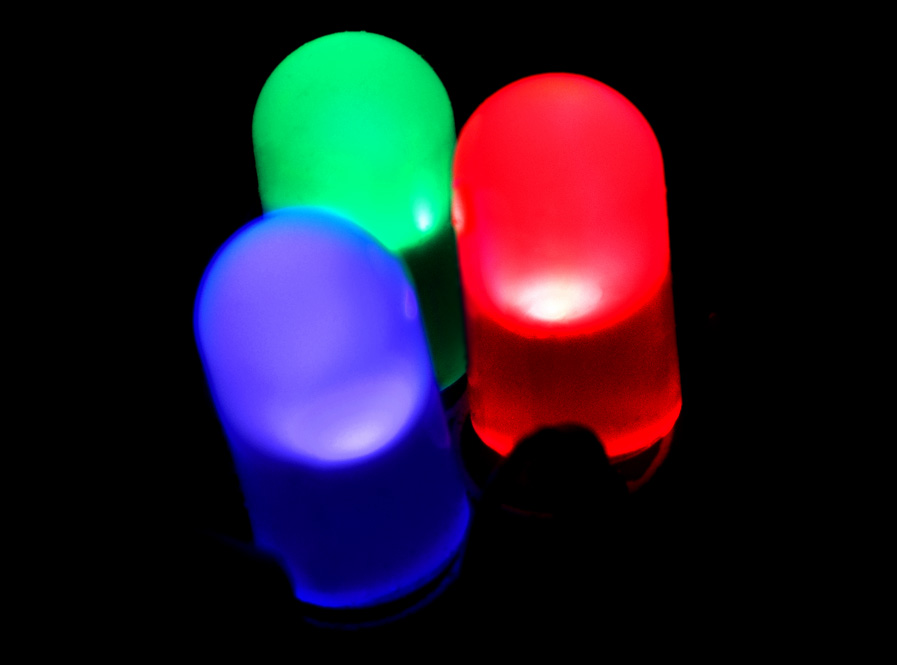
\includegraphics[width=0.5\textwidth]{Immagini/led.jpg}
    \caption{Led}
    \label{fig:my_label}
\end{figure}
\\
Tale led sar\`a posto direttamente sul \textbf{real robot}.


%==Analisi requisito 4: Led Hue Lamp ==================================================================
\subsubsection{Analisi requisito 4: Led Hue Lamp}.
\label{ReqAnalysis4LHL}
\vspace*{1ex}
\\
La lampada HUE \`e una lampada controllabile remotamente.
In particolare per comunicare usa \textit{Zigbee Lighting protocol} e pu\`o essere controllata attraverso un'applicazione smartphone mediante connessione wi-fi.
\begin{figure}
    \centering
    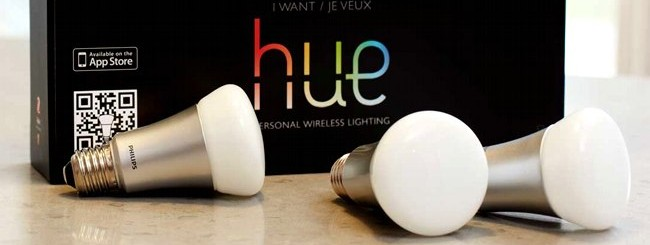
\includegraphics[width=0.6\textwidth]{Immagini/lampade}
    \caption{HUE}
    \label{fig:my_label}
\end{figure}

\pagebreak
%==Analisi requisito aggiuntivo  ==================================================================
\subsection{Analisi requisito aggiuntivo}
\label{ReqAnalysisAgg}
\textit{Moreover, the robot must stop its activity when one of the following conditions apply:
\begin{itemize}
    \item \textbf{R-Stop}: an authorized user has sent a STOP command by using the console.
    \item \textbf{R-TempKo}: the value temperature of the city becomes higher than the prefixed value.
    \item \textbf{R-TimeKo}: the current clock time is beyond the given interval.
    \item \textbf{R-Obstacle}: the robot has found an obstacle that it is unable to avoid.
    \item \textbf{R-End}: the robot has finished its work.
\end{itemize}}

Questo requisito \`e aggiuntivo in quanto, come gi\`a si poteva dedurre dai requisiti precedenti, il committente puntualizza quando il robot ( virtuale o fisico ) deve fermarsi.\\
\vspace*{1ex}
In particolare:
\begin{itemize}
    \item quando l'utente autenticato invia un comando di \textbf{stop} (requisito 1);
    \item quando il valore della \textbf{temperatura} supera un certo valore prefissato (requisito 2);
    \item quando l'\textbf{orario} \`e al di fuori di un intervallo prefissato (requisito 3);
    \item quando il robot si trova davanti ad un \textbf{ostacolo} che non riesce ad evitare (requisito 4);
    \item quando il robot \textbf{termina} il lavoro.
\end{itemize}

%==Analisi requisito aggiuntivo  ==================================================================
\subsection{Analisi requisito 5}
\label{ReqAnalysis5}
\textit{During its work, the robot can \textbf{optionally}
\begin{itemize}
    \item \textbf{R-Map}: build a map of the room floor with the position of the fixed obstacles. Once built, this map can be used to define a plan for an (optimal) path from the start-point to the end-point.
\end{itemize}}

Da questo requisito si deduce che il robot deve tener traccia del suo movimento per poter disegnare la mappa della stanza, tenendo conto di eventuali \textbf{ostacoli fissi}. Inoltre, una volta che il robot \`e riuscito a costruire la mappa della stanza, dovr\`a pianificare il percorso ottimo da effettuare per raggiungere l'\textit{end-point} a partire dallo \textit{start-point}.
\pagebreak


%===========================================================================

%Requisito 1==========================================================
\section{Requisito 1}
\label{Req1}
%Requisito 1: Analisi del problema ==========================================================
\subsection{Analisi del problema}
\label{AnalisidelproblemaReq1}

Dall'analisi del \textit{requisito uno} emerge che la struttura del sistema avr\`a di sicuro due componenti:
\begin{itemize}
    \item \textbf{robot};
    \item \textbf{console}.
\end{itemize}
La loro \textbf{interazione} avviene mediante lo \textbf{scambio di messaggi}, preferiti rispetto agli eventi, in quanto nel modello a scambio di messaggi c'\`e una bassa probabilit\`a di perdita dell'informazione. Ci\`o dipende dal fatto che tutti i messaggi verranno messi all'interno di una coda nel caso in cui il ricevente sia gi\`a occupato. Inoltre gli eventi potrebbero avere pi\`u di un destinatario, ma non \`e questo il caso, in quanto si presume che la console lavori con un robot alla volta.\\
Dall'analisi dei requisiti si deduce che la console lavorer\`a in un \textbf{contesto separato} rispetto a quello del robot, in quanto sar\`a possibile che entrambi lavorino su dei nodi separati.\\
Per realizzare un prototipo utilizzeremo un linguaggio custom realizzato dalla nostra software house chiamato \textbf{\qa}.


%Analisi del problema: Console ==========================================================
\subsubsection{Analisi del problema: Console} .
\label{AnalisidelproblemaReq1Console}
\vspace*{1ex}
\\
Prima di realizzare un prototipo della console, si assume che essa abbia gi\`a verificato l'identit\`a dell'utente e che quindi solo chi autorizzato possa inviare i comandi
\textbf{startBot} e \textbf{stopBot}.
Utilizzando il linguaggio custom, realizziamo un prototipo che simuler\`a il comportamento della console e quindi i suoi relativi comandi.\\
\begin{figure}
    \centering
    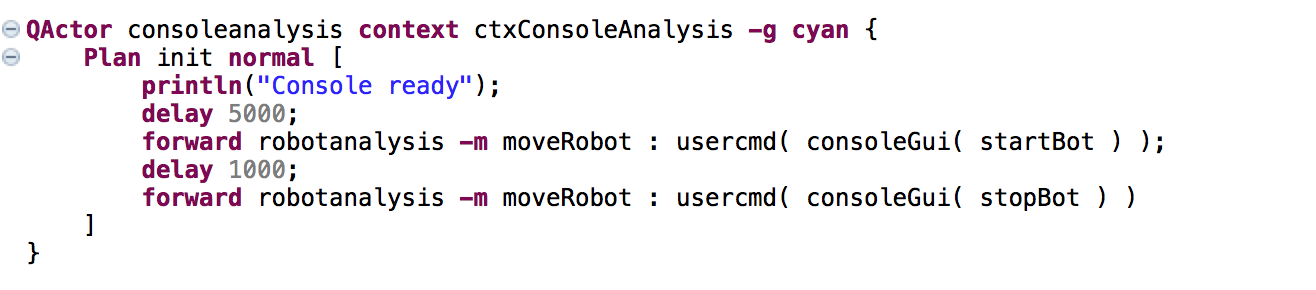
\includegraphics[width=1\textwidth]{Immagini/console(requisito1).png}
    \caption{\qa console}
    \label{fig:my_label}
\end{figure}
\vspace*{1ex}
\\
Tale prototipo ci aiuter\`a ad effettuare un test sul funzionamento corretto dello scambio di messaggi, in questo caso \textbf{consoleGui(CMD)}, tra robot e console. 

%Analisi del problema: Robot ==========================================================
\subsubsection{Analisi del problema: Robot} .
\label{AnalisidelproblemaReq1Robot}
\vspace*{1ex}
\\
Per avere un prototipo completo che riesca a simulare il requisito uno in maniera completa, abbiamo creato un ulteriore \qa che vada a simulare il comportamento del robot.\\
\begin{figure}
    \centering
    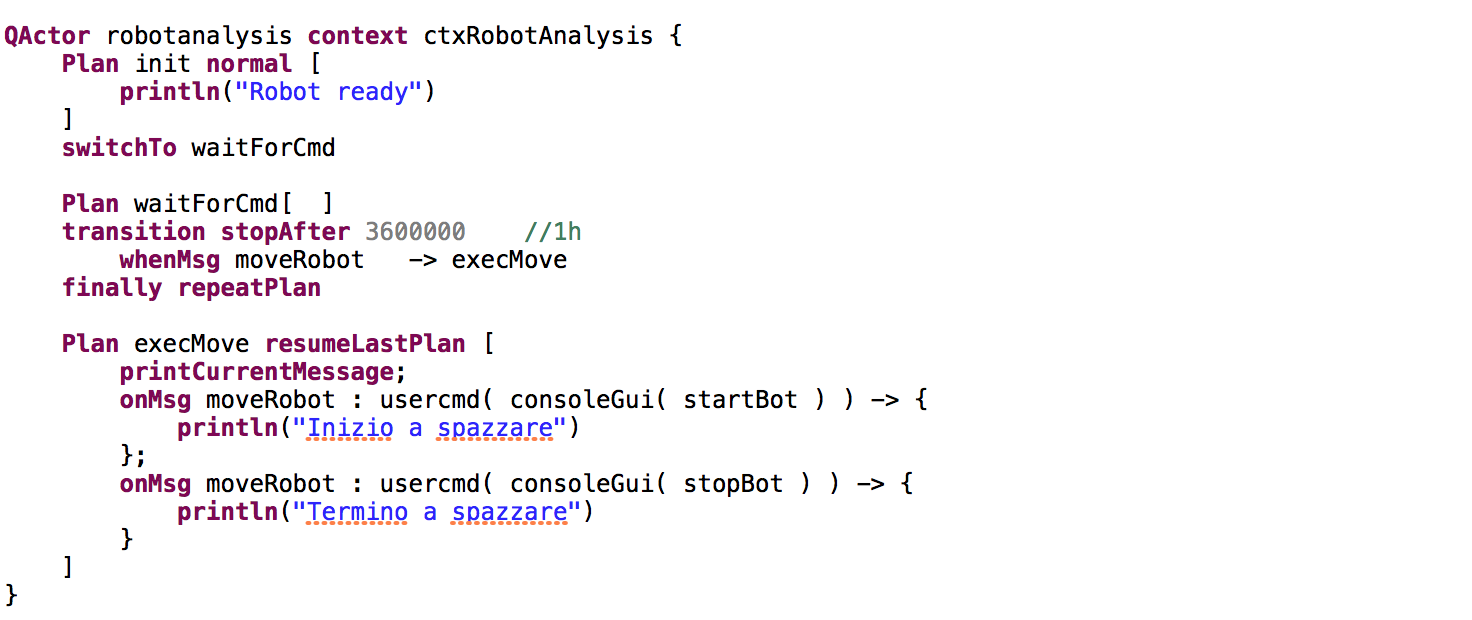
\includegraphics[width=1\textwidth]{Immagini/Robot(requisito1).png}
    \caption{\qa robot}
    \label{fig:my_label}
\end{figure}
\vspace*{1ex}
\\
In particolare:
\begin{itemize}
    \item ogni volta che il robot ricever\`a un messaggio di \textbf{start}, stamper\`a la seguente stringa: \textit{Inizio a spazzare}
    \item ogni volta che il robot ricever\`a un messaggio di \textbf{stop}, stamper\`a la seguente stringa:
    \textit{Termino di spazzare}
\end{itemize}
Il test, per essere il pi\`u fedele possibile all'ambiente reale, si effettuer\`a eseguendo il protipo della console e quello del robot su contesti separati, in modo da poter anche simulare un \textbf{ambiente distribuito}. 

\pagebreak
%Requisito 1: Progettazione========================================================
\subsection{Progettazione}
\label{ProgettazioneReq1}
In fase di progettazione per riuscire ad avere un'idea di come poter procedere poi nell'implementazione, si \`e deciso di realizzare una struttura come quella illustrata nella figura \hyperref[fig:RobotScheme]{\ref{fig:RobotScheme}}.\\
\begin{figure}
    \centering
    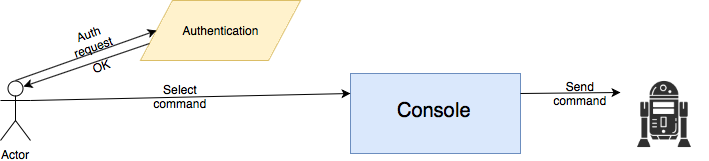
\includegraphics[width=1\textwidth]{Immagini/SchemaRobot.png}
    \caption{Struttura iniziale}
    \label{fig:RobotScheme}
\end{figure}
\vspace*{1ex}
\\
Dal grafico si pu\`o notare come non viene fatta una distizione tra \textit{robot reale} e \textit{robot virtuale}, in quanto i comandi inviati dalla console verranno "catturati" da entrambi e, poi interpretati dal robot attualmente attivo.\\
Per realizzare un comportamento del genere si utilizza una tecnologia che segue il modello \textbf{publish/subscribe}: in questo modello, mittenti e destinatari di messaggi dialogano attraverso un tramite, detto \textbf{dispatcher} o \textbf{broker}. Il mittente di un messaggio (detto publisher) non deve essere consapevole dell'identit\`a dei destinatari (detti \textbf{subscriber}); esso si limita a "pubblicare" il proprio messaggio al dispatcher. La tecnologia scelta per realizzare questo modello \`e \textbf{MQTT} ( Message Queue Telemetry Transport ).\\
Nella figura \hyperref[fig:pubsub]{\ref{fig:pubsub}} \`e mostrato come, a grandi linee, dovrebbe funzionare tale modello.
\begin{figure}
    \centering
    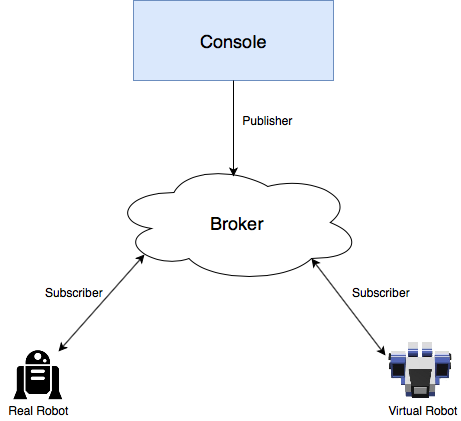
\includegraphics[width=0.45\textwidth]{Immagini/Mqtt.png}
    \caption{Modello publish/subscribe}
    \label{fig:pubsub}
\end{figure}
\pagebreak

%Progettazione: Robot ======================================================================
\subsubsection{Progettazione: Robot}.
\label{ProgettazioneReq1Robot}
\vspace*{1ex}
\\
Dall'analisi dei requisiti ci siamo accorti che non esiste una sola versione del robot, ma due:
\begin{itemize}
    \item una \textbf{Virtuale} (virtual robot);
    \item una \textbf{Reale} (real robot).
\end{itemize}
Quindi prima di procedere con la progettazione del robot \`e stata fatta la seguente considerazione: visto che le versioni sono due, ci conviene fare gi\`a a partire dalla progettazione del requisito uno, un modello che catturi gli aspetti essenziali di entrambi.\\
Per questo motivo nelle seguenti sezioni analizzeremo i due modelli corrispondenti alle due versioni.

%Progettazione: Real Robot ======================================================================
\subsubsection{Progettazione: Adapter Real Robot}.
\label{ProgettazioneReqRR}
\vspace*{1ex}
\\
Il robot sar\`a realizzato mediante le seguente componenti (\textbf{Fig.} 7):
\begin{itemize}
    \item 1 x Raspberry pi 3;
    \item 1 x Bridge motor (L298N) che permetter\`a la gestione dei due motori (avanti e indietro);
    \item 2 x Gear Motor;
    \item 1 x Sesore ultrasonico (HC-SR04);
    \item 1 x green led;
    \item 1 x power bank.
\end{itemize}
\begin{figure}
    \centering
    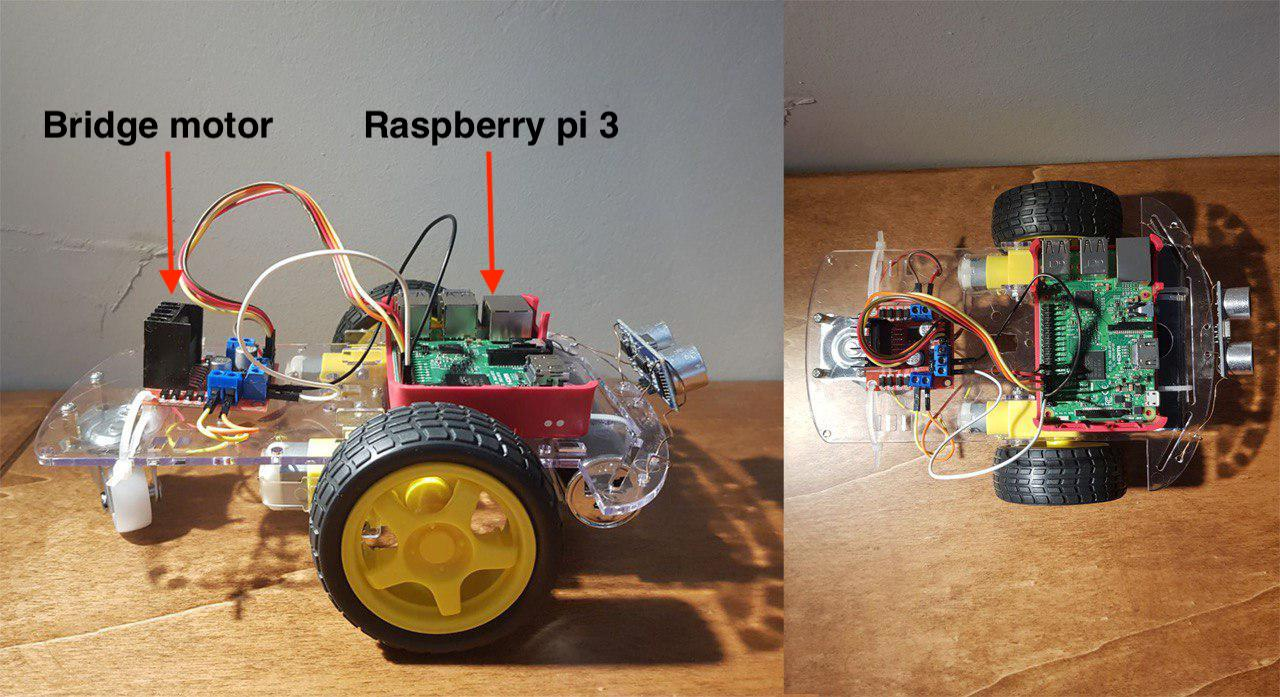
\includegraphics[width=1\textwidth]{Immagini/RealRobot.jpg}
    \caption{Real Robot}
    \label{fig:my_label}
\end{figure}
\vspace*{1ex}
\\
Il robot \`e una componente IoT del sistema, questo significa che deve essere in grado di connettersi alla rete e di eseguire dei compiti inviati in remoto dalla console. Per diventare una componente IOT, il \textbf{Real Robot} usa una \textbf{raspberry pi 3} che, oltre a essere fondamentale per la gestione del movimento del robot, sar\`a fondamentale per il collegamento del robot al sistema distribuito.\\
Le restanti componenti saranno utili per soddisfare i requisiti successivi; avendo adottato un procedimento incrementale, queste verranno analizzate quando ce ne sar\`a bisogno.\\
Per rendere il prototipo funzionante il real robot verr\`a modellato, attraverso il linguaggio custom (\qa) fornito dalla nostra software house, come mostrato in figura.\\
\begin{figure}
    \centering
    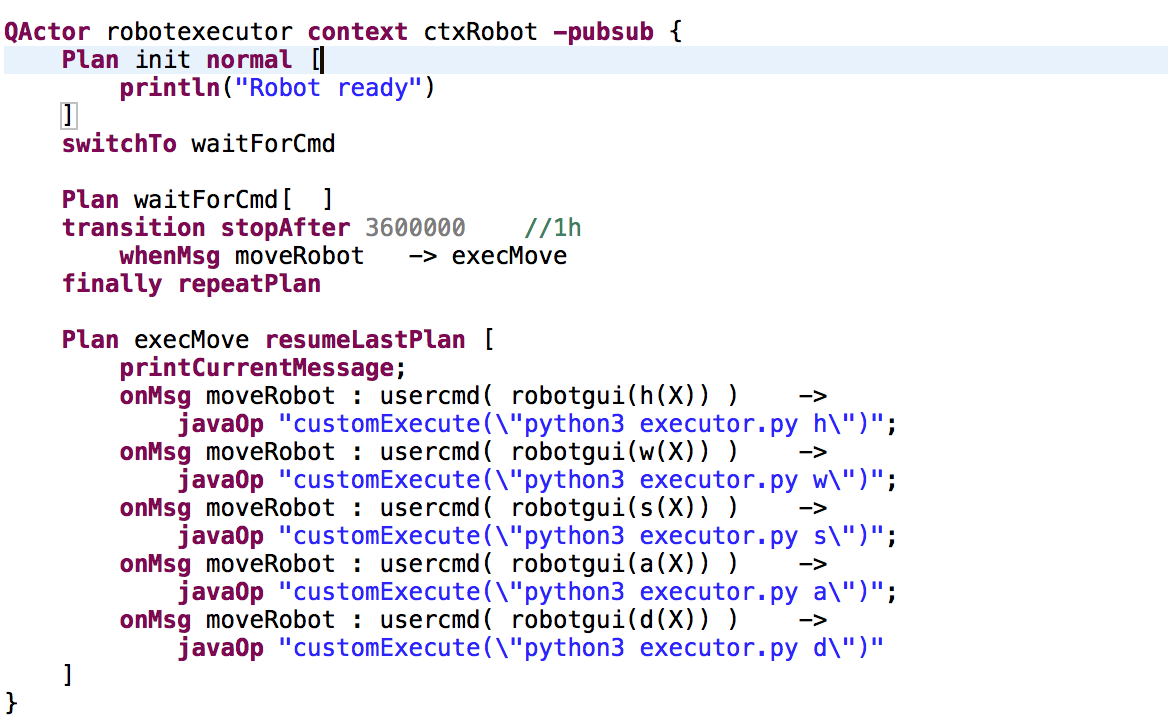
\includegraphics[width=1\textwidth]{Immagini/robotexecutor(req1).png}
    \caption{Modello Robot Reale}
    \label{fig:RRmodel}
\end{figure}
\pagebreak
Dal modello (Fig. \hyperref[fig:RRmodel]{\ref{fig:RRmodel}}) si pu\`o notare come il robot sia sempre in attesa di un messaggio ( \textbf{moverobot}) che racchiude la mossa che il robot dovr\`a effettuare. Tale messaggio \`e analogo al messaggio (\textbf{consoleGui}) utilizzato in fase di testing dei messaggi nell'analisi del problema.\\
Da notare che ogni qual volta che viene ricevuto un messaggio viene eseguita la seguente riga:\\
\textcolor{red}{\textbf{javaOp}} \textcolor{blue}{"customExecute( "python3 executor.py h ")"};\\
Questa viene aggiunta soltanto dopo aver testato che i messaggi arrivassero correttamente e dopo aver testato che lo script \textit{python}, che verr\`a analizzato in fase di implementazione, funzionasse correttamente.
Questo modello verr\`a poi eseguito direttamente sulla raspberry e avr\`a la funzione di \textbf{adapter}, in quanto far\`a corrispondere ai comandi inviati dalla console l'esecuzione dello script python, di cui parleremo in fase di implementazione.


% Progettazione: Virtual Robot ======================================================================
\subsubsection{Progettazione: Adapter Virtual Robot}.
\label{ProgettazioneReq1VR}
\vspace*{1ex}
\\
Il virtual robot \`e un'applicazione web fornita dalla software house, che ci sar\`a utile sia per simulare i comportamenti del robot fisico in un ambiente virtuale, sia per effettuare operazioni di testing, che simulino l'ambiente reale.\\
\begin{figure}
    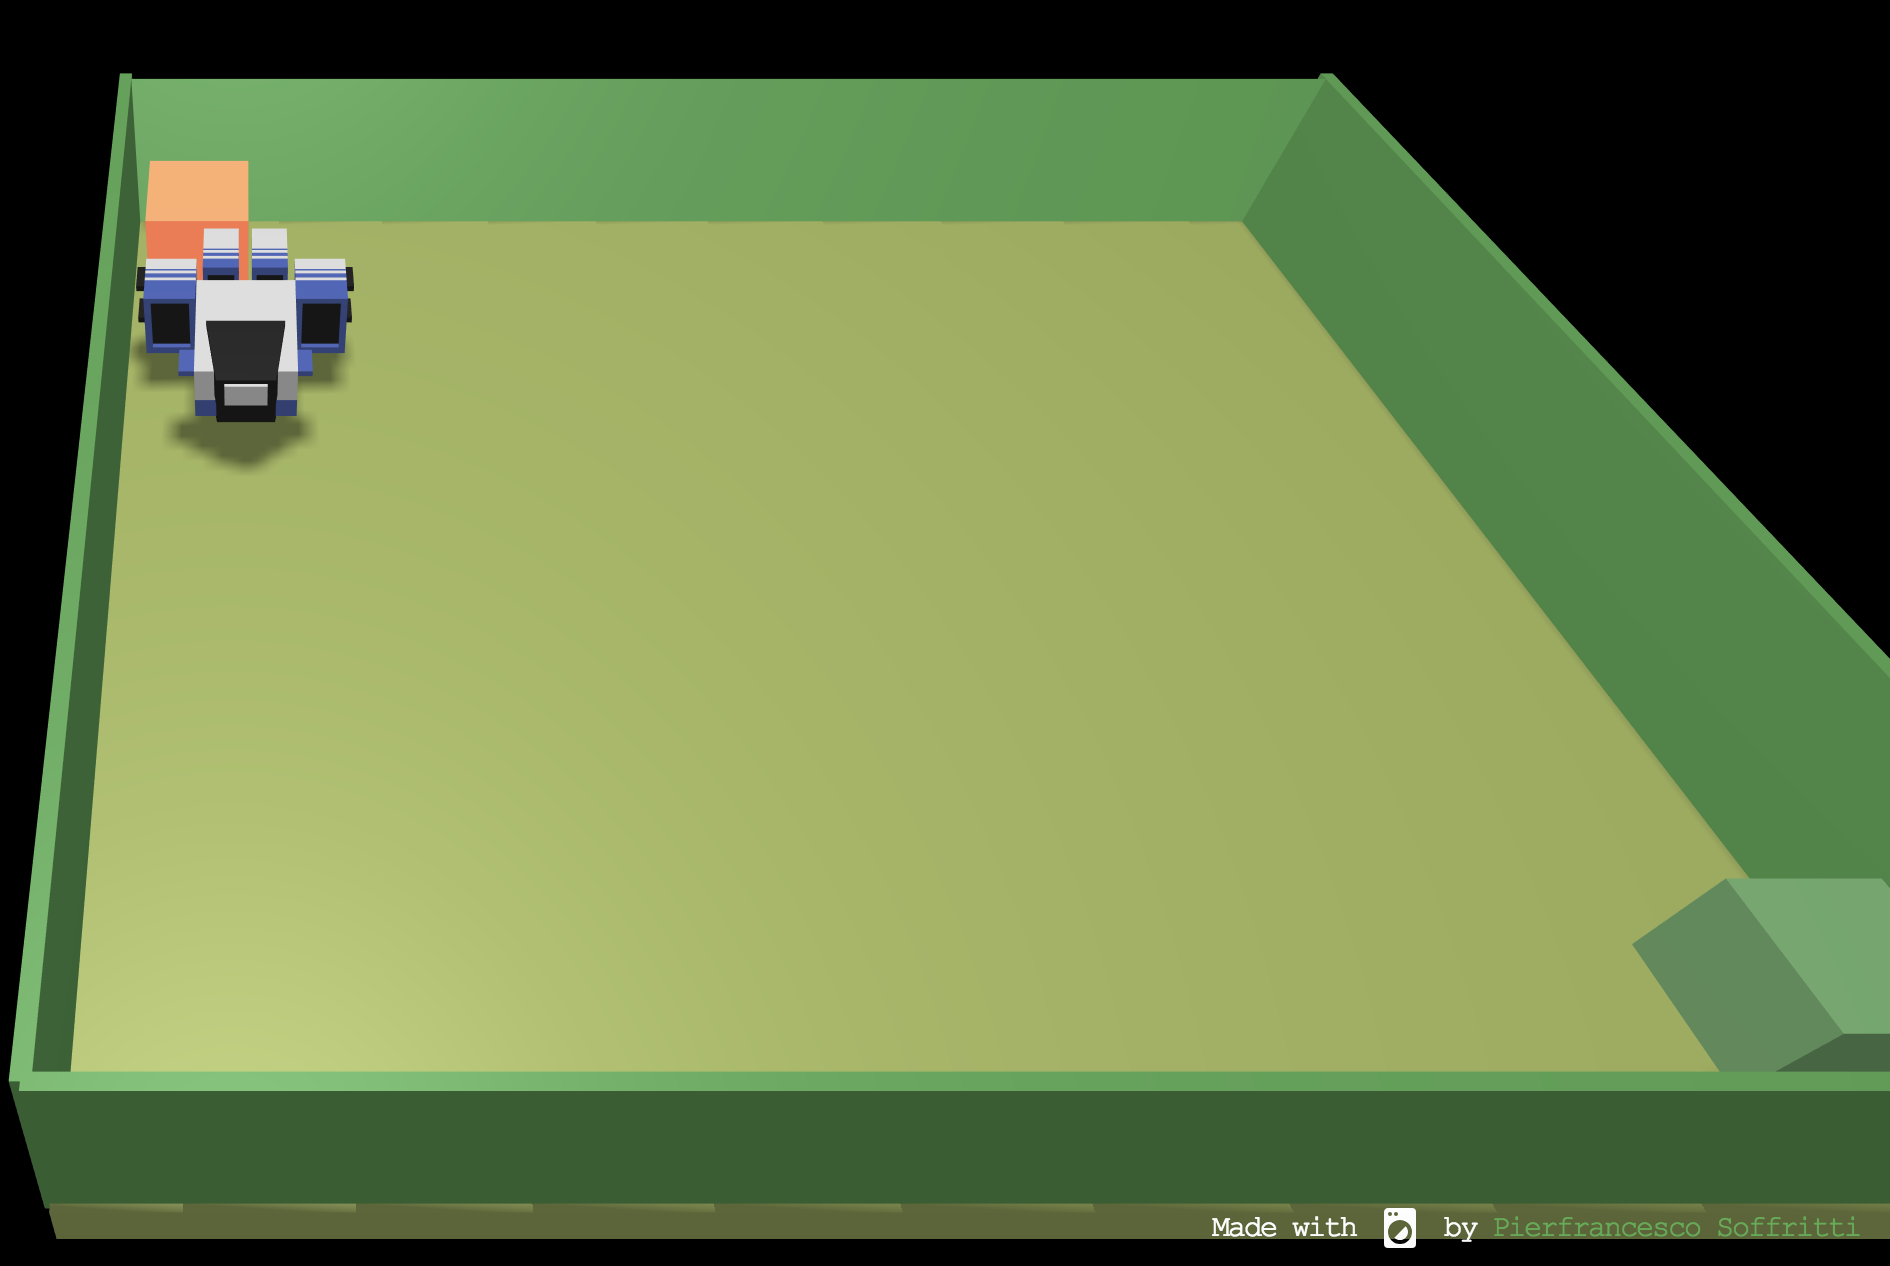
\includegraphics[width=1\textwidth]{Immagini/VirtualRobot.png}
    \caption{Virtual Robot}
    \label{fig:my_label}
\end{figure}
\vspace*{1ex}
\\
Come si pu\`o notare dalla figura, sono presenti due sonar (start-point e end-point) che delimitano la stanza in cui il virtual robot potr\`a muoversi. Da ci\`o ne consegue che la stanza simulabile potr\`a essere o un quadrato o un rettangolo.\\
Inoltre in quest'ambiente virtuale, attraverso degli opportuni file messi a disposizione dal componente, sar\`a possibile inserire ostacoli fissi (tavoli, armadi, sedie, ecc.) e ostacoli mobili (animali, persone, palloni, ecc.) per pemettere una simulazione pi\`u accurata.
Come nel caso del real robot, anche quest'ultimo \`e dotato di un sonar in grado di rilevare gli ostacoli. Infatti, ogni qualvolta che verr\`a incontrato un ostacolo, il virtual robot pubblicher\`a attraverso un \textbf{software \java} ( \textbf{clientTCP} fornito dalla software house) sul \textit{broker} di \textbf{mqtt} il seguente messaggio:
\\
\textit{msg(sonarDetect,event,virtualrobot\_executorctrl, none,sonarDetect(wallLeft,soffritti),22)}
\\
\vspace*{1ex}
Per rendere il prototipo funzionante il robot virtuale \`e stato modellato come in figura 10.\\
\begin{figure}
    \centering
    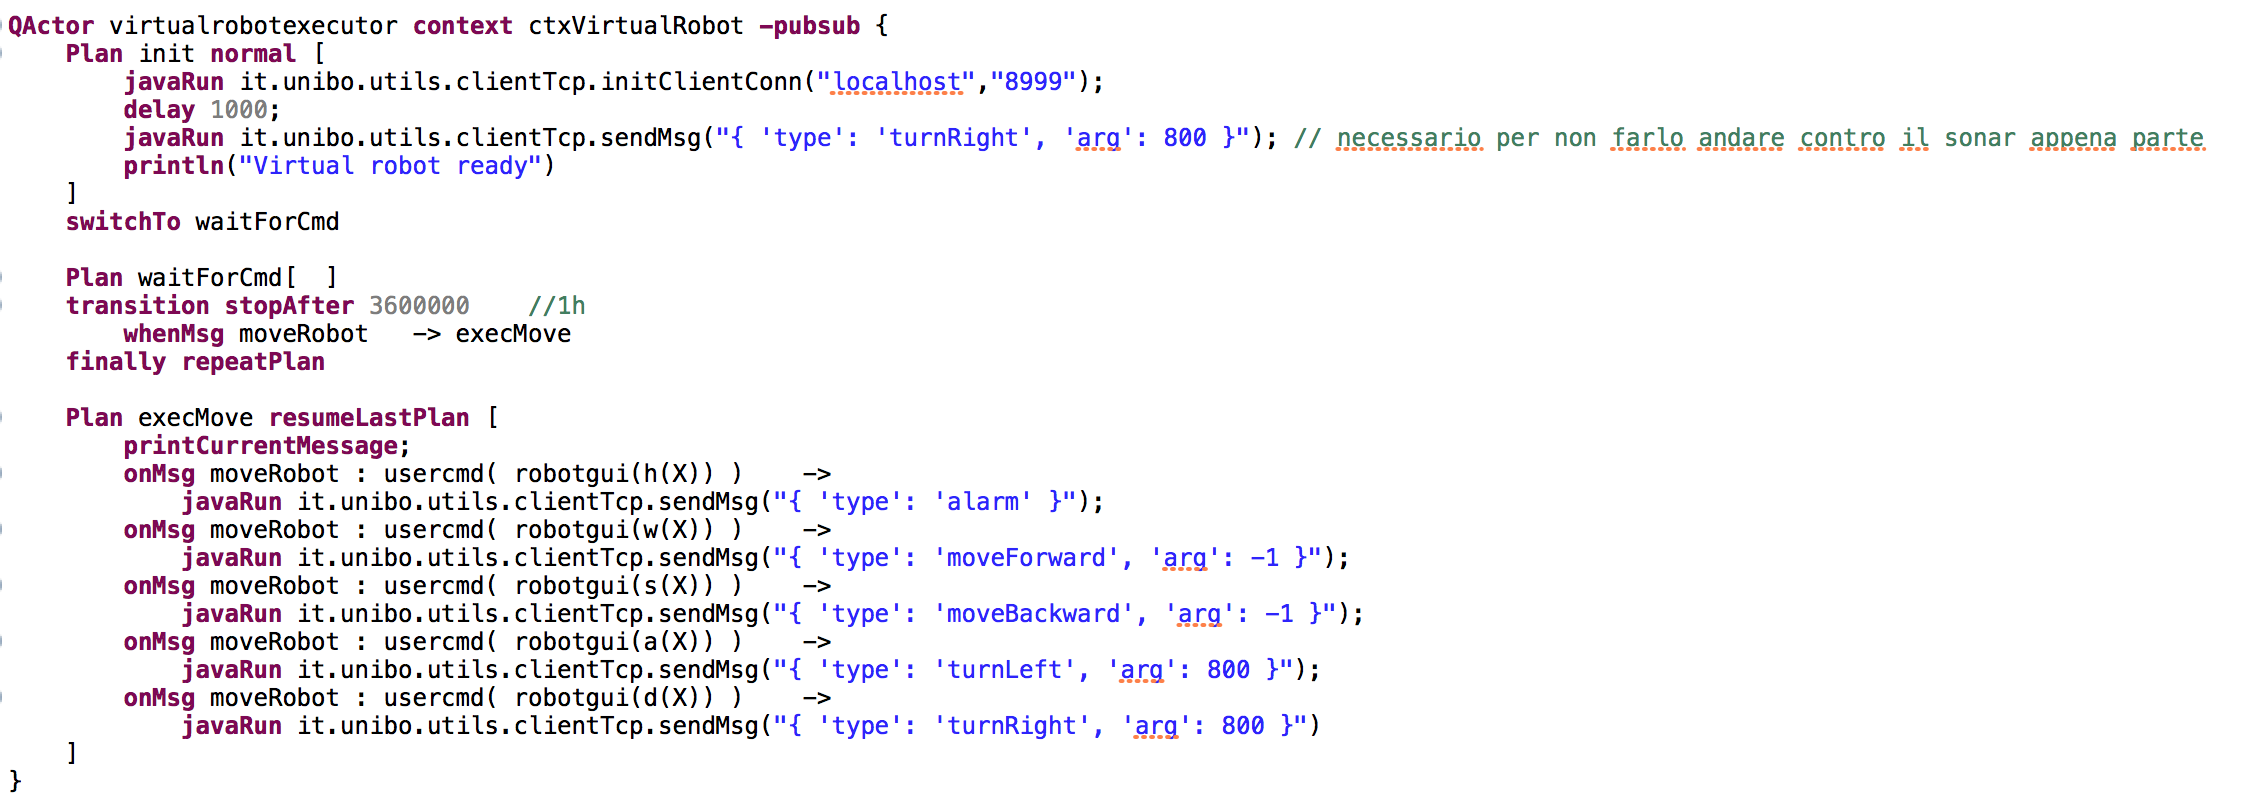
\includegraphics[width=1\textwidth]{Immagini/virtualrobotexecutor(requisito1).png}
    \caption{Modello Robot Virtuale}
    \label{fig:my_label}
\end{figure}
\\
\vspace*{1ex}
Come nel caso del robot reale, anche in questo caso il messaggio usato \`e \textbf{moveRobot} e, come nel caso precedente, prima dell'invio del messaggio al robot virtuale fornito dalla software house sono stati effettuati dei test sul corretto funzionamento dei messaggi. 
Prima di andare a vedere come sono stati progettati internamente il blocco \textbf{console} e il blocco \textbf{authentication}, verranno introdotte alcune tecnologie utilizzate.


% Progettazione: Tecnologie ======================================================================
\subsubsection{Progettazione: Tecnologie} .
\label{ProgettazioneReq1Tec}
\vspace*{1ex}
\\
La console verr\`a realizzata mediante \textbf{ReactJS} una tecnologia recente, scritta in JavaScript, che permette di realizzare, lato frontend, una '\textit{One page application}', ovvero un'applicazione web che carica la pagina solo la prima volta che l'utente la richiede e poi aggiorna il contenuto in maniera dinamica andando ad iniettare i componenti senza bisogno di ricaricare la stessa. La scelta di questa tecnologia \`e motivata dal fatto che il trend attuale \`e proprio quello di realizzare queste cosidette '\textit{One page application}' perch\`e garantiscono una migliore \textbf{user-experience}.\\
Come vedremo successivamente, questa applicazione web necessita di un \textbf{backend} in grado di comunicare con il robot e in grado di memorizzare su di un database i dati dell'utente per verificare l'accesso.\\
Per la realizzazione del backend abbiamo scelto un'altra tecnologia molto utilizzata, \textbf{NodeJS}, una piattaforma scritta in JavaScript che sfrutta il motore di \textbf{Google Chrome V8} per la realizzazione di server web con modello \textbf{asincrono}, detto \textit{event-driven}. Si tratta di un modello in cui, quando si richiedono operazioni "lente"  - come ad esempio le operazioni di I/O (input/output) -, il sistema non resta in attesa del loro completamento, ma continua ad eseguire il codice sottostante;  solo quando tale operazione termina si esegue una cosidetta '\textit{callback}' con le istruzioni da eseguire.\\
Per la gestione del database la tecnologia che \`e stata scelta \`e \textbf{MongoDB}, ovvero un database non relazionale (\textbf{NoSQL}) che  si allontana dalla struttura tradizionale basata su tabelle dei database relazionali a favore di documenti in stile JSON con schema dinamico. Considerando le operazioni che devono essere effettuate e le tecnologie utilizzate per la realizzazione del backend, questa risulta essere la migliore alternativa in termini di performance, costi e anche supporto da parte della community.
\pagebreak

% Progettazione: Authentication ======================================================================
\subsubsection{Progettazione: Authentication} .
\label{ProgettazioneReq1Auth}
\vspace*{1ex}
\\
L'autenticazione, successiva alla registrazione dell'utente mediante la scelta di \textbf{username} e \textbf{password}, si compone dei seguenti passi:
\begin{enumerate}
    \item L'utente inserisce, nella pagina di login della web application, '\textbf{username} e  \textbf{password};
    \item l'applicazione richiede al web server di verificare l'esistenza dell'username e la validit\`a della password inseriti dall'utente;
    \item se i dati sono validi, il web server restituisce un token di accesso valido per un'ora e che permette all'utente di accedere alla console.
\end{enumerate}

% Progettazione: Console ======================================================================
\subsubsection{Progettazione: Console} .
\label{ProgettazioneReq1Console}
\vspace*{1ex}
\\
\begin{figure}
    \centering
    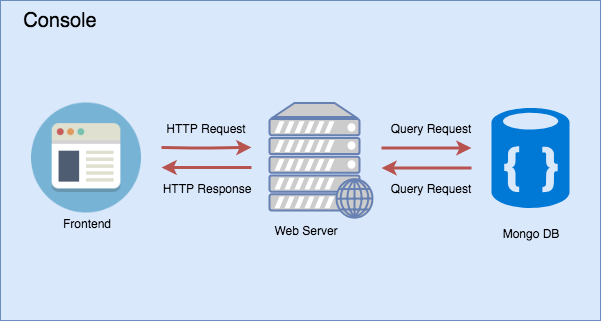
\includegraphics[width=0.8\textwidth]{Immagini/Console-diagram.png}
    \caption{Struttura console}
    \label{fig:my_label}
\end{figure}
\vspace*{1ex}
La console si compone di tre componenti:
\begin{enumerate}
    \item \textbf{Frontend} realizzato con \textbf{ReactJS}, interfaccia attraverso cui l'utente potr\`a interagire con il sistema;
    \item \textbf{Web Server} realizzato con \textbf{NodeJS}, che eseguir\`a le richieste effettuate dal frontend;
    \item \textbf{Data Base} realizzato utilizzando \textbf{MongoDB}, per memorizzare le informazioni relative all'utente autenticato.
\end{enumerate}

\pagebreak
%Requisito 1: Implementazione========================================================
\subsection{Implementazione}
\label{ImplementazioneReq1}
% Implementazione: Authentication ======================================================================
\subsubsection{Implementazione: Authentication} .
\label{ImplementazioneReq1Auth}
\vspace*{1ex}
\\
A livello implementativo l'autenticazione \`e stata realizzata:
\begin{itemize}
    \item lato \textbf{frontend} mediante un componente React contente il form di login, che prender\`a i dati inserti dall'utente e li invier\`a al webserver tramite richiesta HTTP;
    \item lato \textbf{backend} mediante controllo dei dati inseriti dall'utente. A questo punto se i dati inseriti sono validi si controlla se l'username \`e presente all'interno del database e che la password sia quella corretta. Se tutto \`e andato a buon fine verr\`a restituito un \textbf{JSON Web Token} (JWT), che permetter\`a all'utente di rimanere autenticato per un'ora.
\end{itemize}\\
\begin{figure}
    \centering
    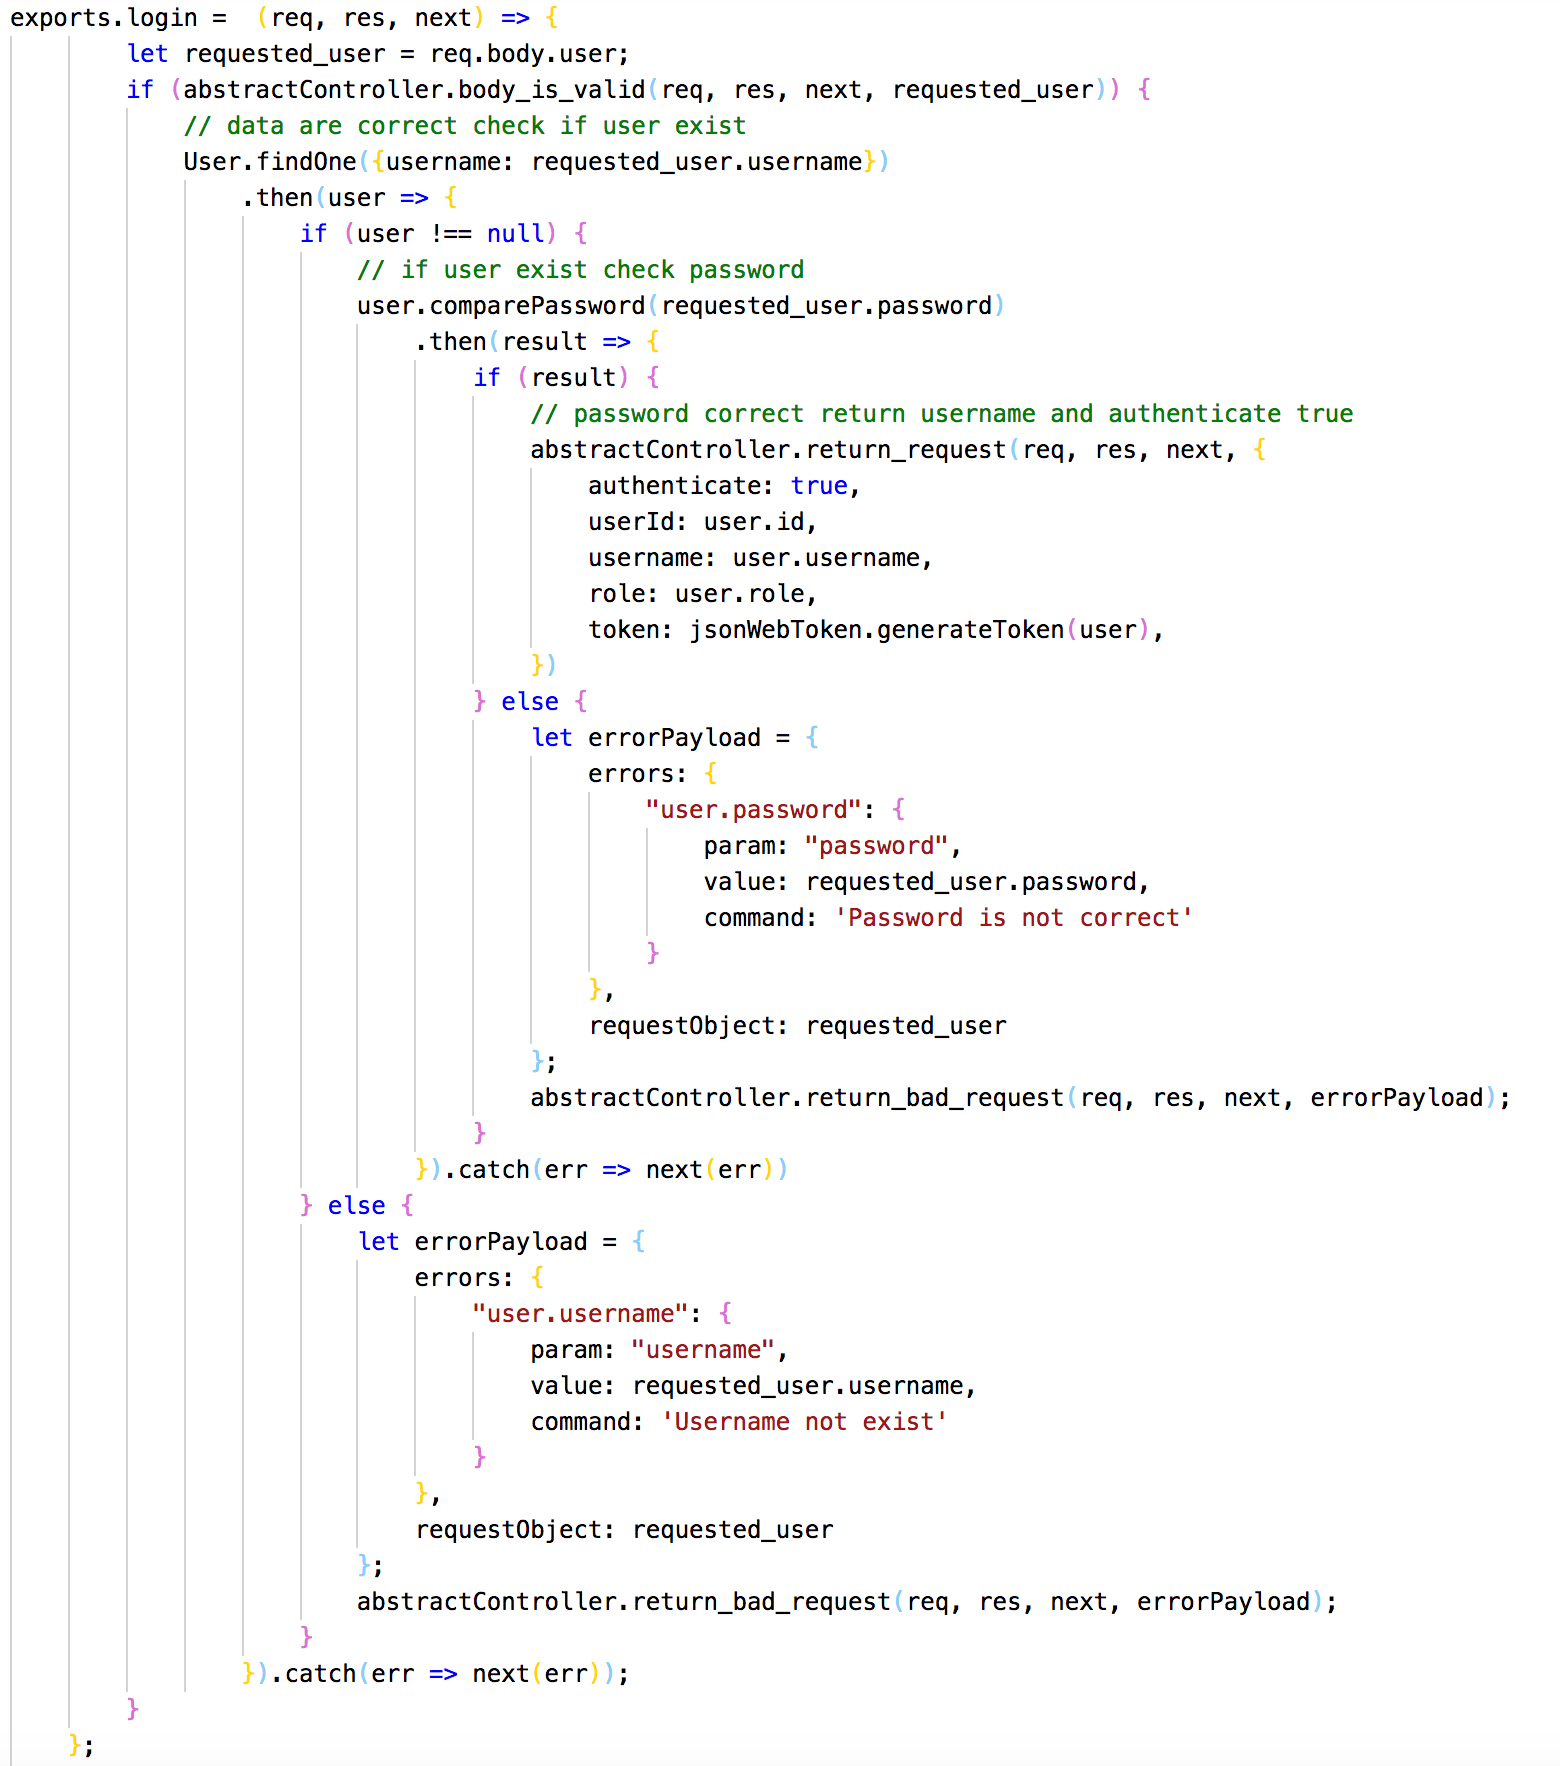
\includegraphics[width=0.85\textwidth]{Immagini/Login-code.png}
    \caption{Implementazione Login}
    \label{fig:my_label}
\end{figure}
\vspace*{1ex}
\\
Il JWT \`e una stringa codificata in \textbf{BASE64} composta da 3 componenti:
\begin{itemize}
    \item La prima contiene informazioni sull'algoritmo usato per generare la firma di verifica (Verify Signature);
    \item La seconda parte contiene il payload, ovvero le informazioni relative all'utente e al periodo di validit\`a che si vogliono ottenere quando si decodifica il token;
    \item La terza parte contiene la Verify Signature usata poi per controllare l'effettiva autenticit\`a del token.
\end{itemize}

% Implementazione: Console ======================================================================
\subsubsection{Implementazione: Console} .
\label{ImplementazioneReq1Console}
\vspace*{1ex}
\\
Nell'implementazione della console abbiamo deciso, per completezza, di aggiungere, oltre al comando start e stop, dei comandi che permetteranno all'utente di comandare manualmente il robot.\\
In particolare i comandi sono i seguenti:
\begin{itemize}
    \item \textbf{Forward}: permette al robot di andare avanti;
    \item \textbf{Backward}: permette al robot di andare indietro;
    \item \textbf{Left}: permette al robot di girarsi a sinistra;
    \item \textbf{Right}: permette al robot di girarsi a destra;
    \item \textbf{Stop}: permette al robot di fermarsi (corrisponde al comando di STOP richiesto nei requisiti);
    \item \textbf{Allow Autopilot}: permette al robot di iniziare la pulizia della stanza (corrisponde al comando di START richiesto nei requisiti);
\end{itemize}

\begin{figure}
    \centering
    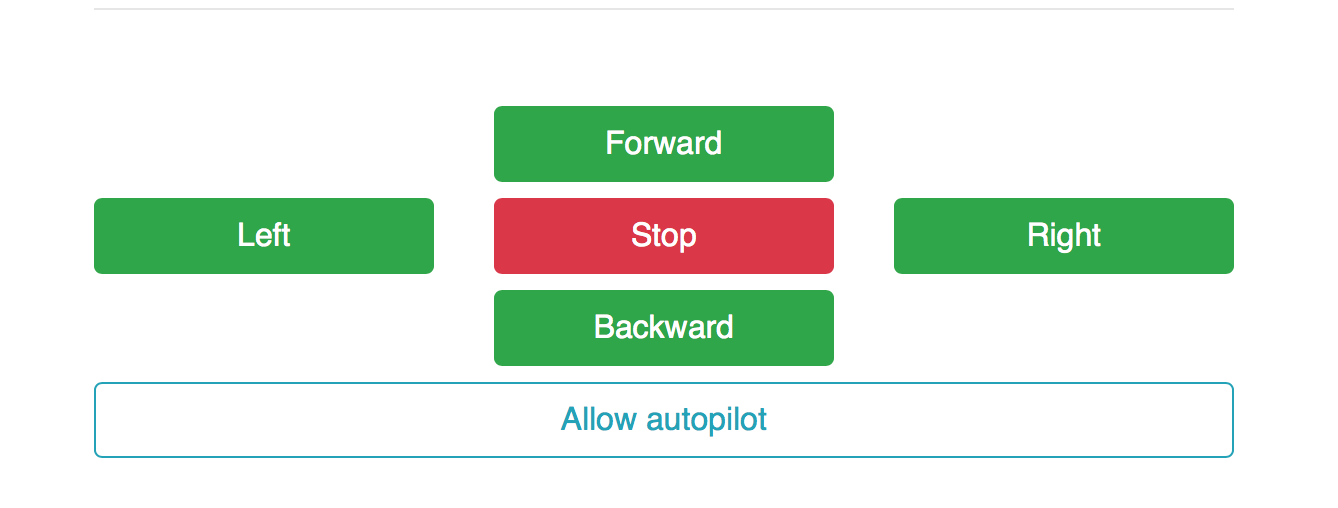
\includegraphics[width=0.9\linewidth]{Immagini/Console.png}
    \caption{Console}
    \label{fig:my_label}
\end{figure}
\vspace*{1ex}
\\
L'ultimo comando non verr\`a implementato in questo momento, ma successivamente, quando si inizier\`a  a pensare sul come il robot debba pulire e costruire la mappa della stanza (vedi \hyperref[Requisito5]{Requisito 5}).\\
Come preannunciato in fase di progettazione, ogni qual volta l'utente autorizzato cliccher\`a su un pulsante messo a disposizione dal frontend, verr\`a inviata una richiesta \textbf{HTTP} al server che a sua volta (come mostrato in figura 6) pubblicher\`a un messaggio sul broker di mqtt, che indicher\`a il movimento che il robot dovr\`a effettuare. In questo modo tutti i robot "iscritti" al broker riceveranno il comando inviato dall'utente.\\
Degno di nota \`e il fatto che il web server sia \textbf{RESTful}. Infatti, ogni volta che esso riceve una richiesta non effettua mai il render di una pagina HTML come risposta, ma semplicemente ritorna una stringa JSON, dove segnala che tutto \`e andato a buon fine.\\
La console cos\`i implementata ce la porteremo avanti fino al termine dell'intero progetto, aggiungendo poi il comando relativo alla pulizia automatica della stanza.
\pagebreak

% Implementazione: Robot ======================================================================
\subsubsection{Implementazione: Robot} .
\label{ImplementazioneReq1Robot}
\vspace*{1ex}
\\
Avendo gi\`a definito in fase di progettazione il modello del \textbf{Virtual Robot} e essendo gi\`a pronto per l'uso visto che viene fornito dalla nostra software house, tratteremo nell'implementazione soltanto ci\`o che permette il movimento del \textbf{Real Robot}. \\
Lo script python sfrutta, per rendere possibile il movimento del robot, la tecnologia \textbf{GPIO} messa a disposizione dalla raspberry.\\
\begin{figure}
    \centering
    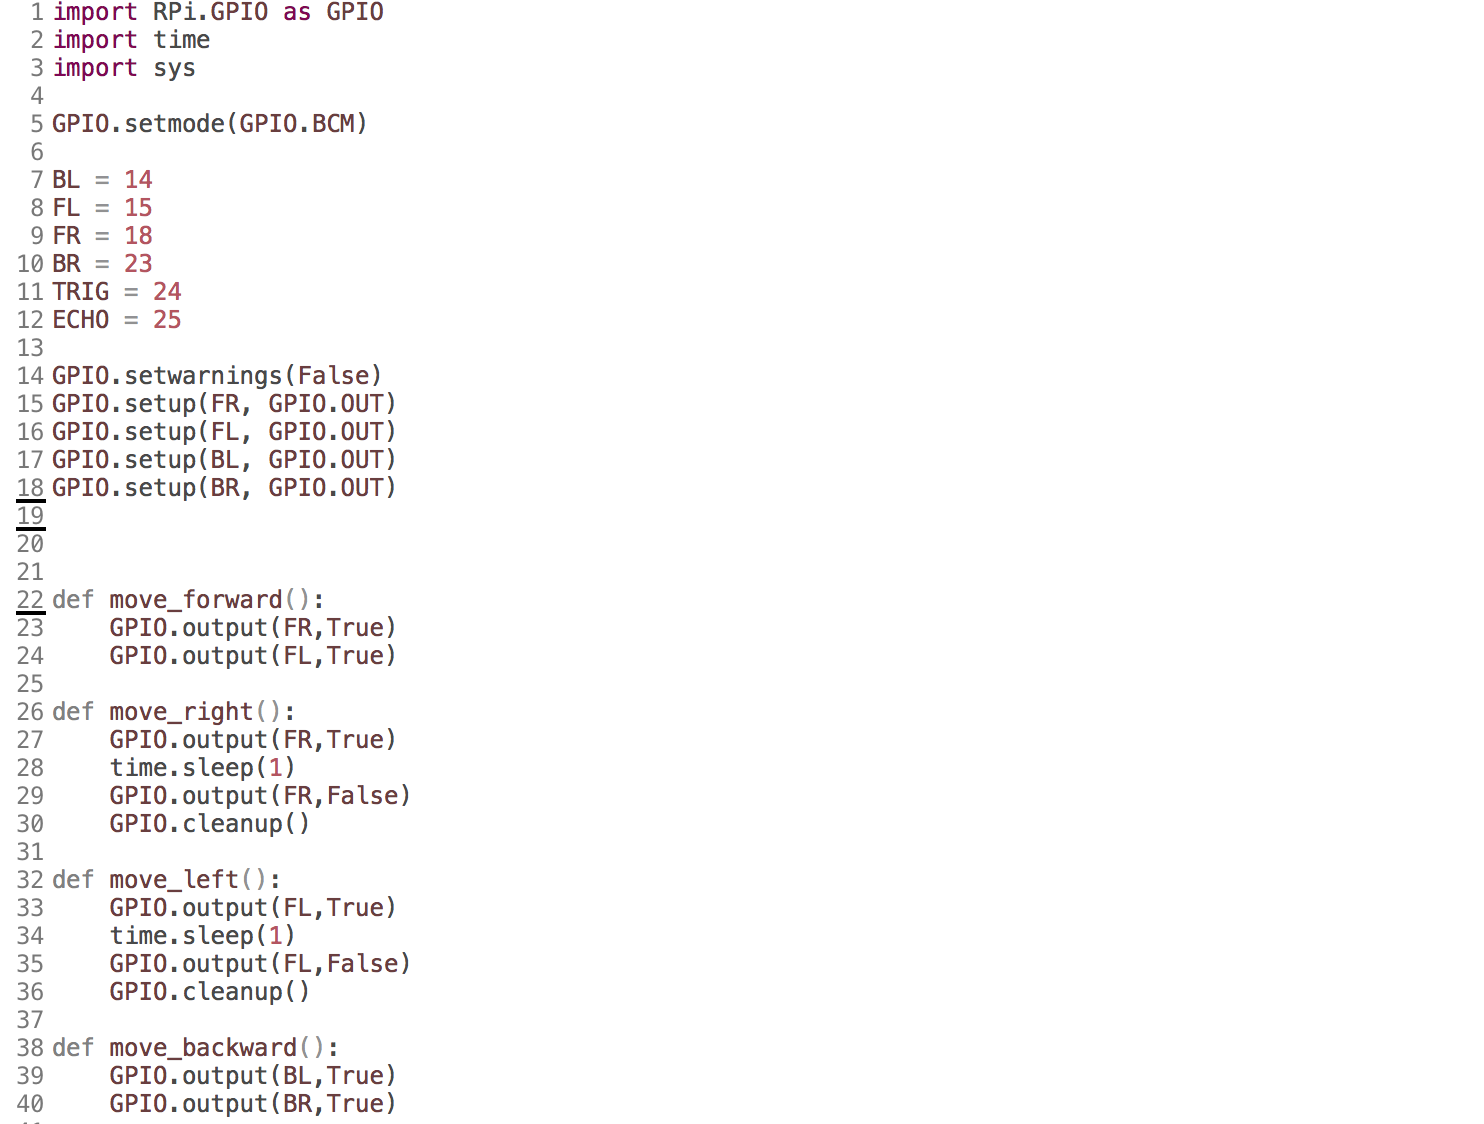
\includegraphics[width=1\textwidth]{Immagini/Scripts/Script(1)req1.png}
    \caption{Script python Parte 1}
    \label{fig:my_label}
\end{figure}
\vspace*{1ex}
\\
Nella prima parte dello script viene stabilito in che modo utilizzare i PIN (\textbf{GPIO.BCM}, tenendo in considerazione la documentazione fornita dalla raspberry) e successivamente quali PIN utilizzare (da notare che i PIN \textbf{TRIG} e \textbf{ECHO} non verranno usati in questa versione dello script). Una volta che sono stati stabiliti quali PIN verranno utilizzati si stabilisce come utilizzarli: \textbf{INPUT} o \textbf{OUTPUT}. Nel nostro caso ci serviranno solo PIN impostati su \textbf{OUTPUT}.\\
Fatto questo vengono definite pi\`u funzioni che definiscono i movimenti che il robot pu\`o effettuare. In questa prima versione i movimenti di rotazione non sono ancora precisi, tuttavia riescono a darci un movimento accettabile per un primo prototipo.
\\
\begin{figure}
   
    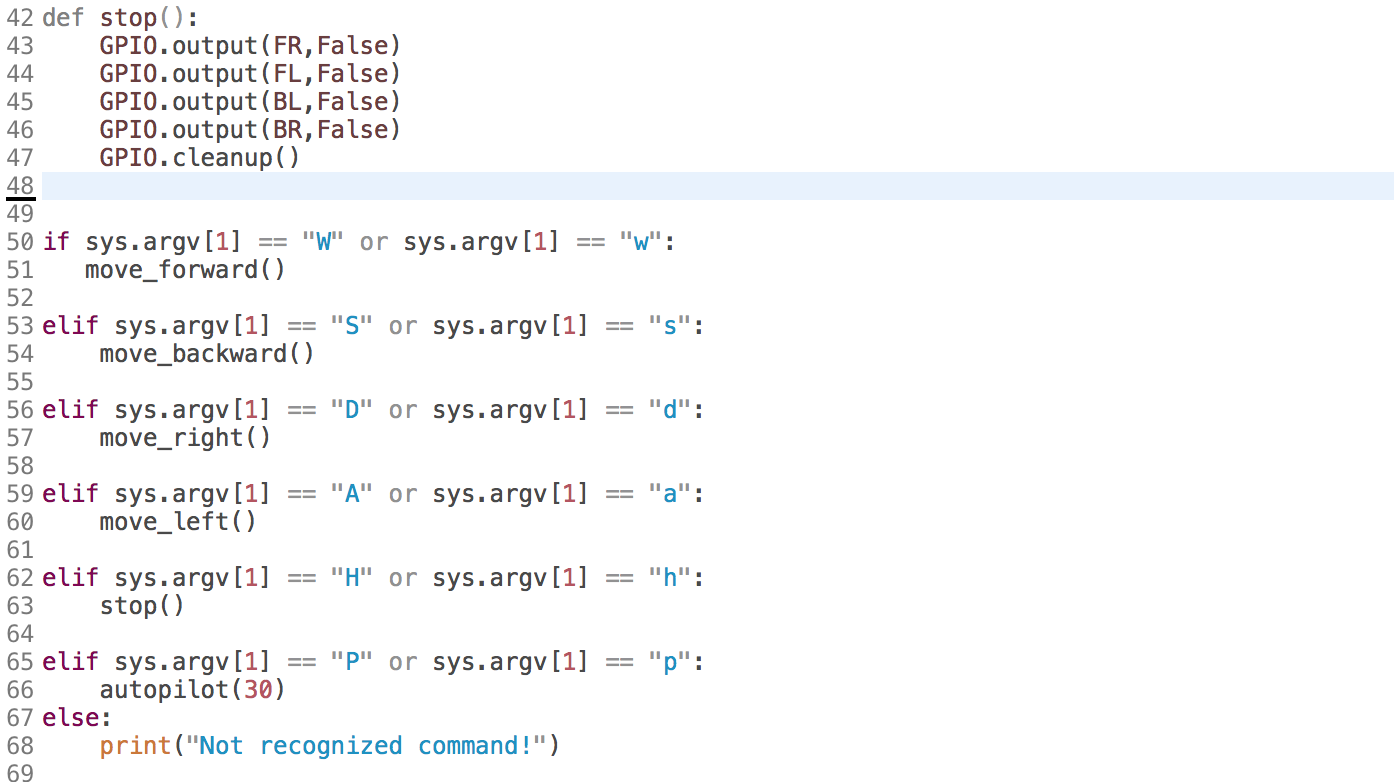
\includegraphics[width=0.8\textwidth]{Immagini/Scripts/Script(2)req1.png}
    \caption{Script python Parte 2}
    \label{fig:my_label}
\end{figure}
\vspace*{1ex}
\\
\textbf{Al termine di questa implementazione abbiamo un primo prototipo funzionante da mostrare al committente.}
\pagebreak

%=Requisito 2===============================================================
\section{Requisito 2}
\label{Requisito 2}
%\textit{\textbf{R-TempOk}: the value temperature of the city is not higher than a prefixedvalue (e.g. 25 degrees Celsius).}
%Requisito 2: Analisi del problema ==========================================================
\subsection{Analisi del problema}
\label{AnalisidelproblemaReq2}
L'analisi del \textit{requisito 2} introduce un vincolo al nostro sistema distribuito, dal momento che - tenendo in considerazione anche l'analisi del requisito aggiuntivo \hyperref[ReqAnalysisAgg]{\ref{ReqAnalysisAgg}} - il \textbf{Robot} potr\`a muoversi solo se il valore della temperatura \`e al di sotto di un certo valore (ad esempio 25 gradi Celsius). \\
Per riuscire ad effettuare la valutazione di questo vincolo bisogna fare delle modifiche a livello strutturale. Infatti risulter\`a pi\`u conveniente introdurre una nuova componente che si occupi soltanto della verifica dei vincoli. In questo modo riusciremo a separare la \textbf{logica} dall'esecuzione dei comandi veri e propri.\\
L'aggiunta di questa nuova componente porter\`a delle modifiche anche nella console, in quanto quest'ultima non dovr\`a pi\`u comunicare direttamente con il robot, ma dovr\`a farlo con la nuova componente introdotta, la quale stabilir\`a se sar\`a possibile o meno effettuare l'azione indicata.\\
Di seguito verr\`a creato un prototipo per effettuare dei test sul funzionamento dei vincoli solo a livello locale.

%Analisi del problema: Mind ==========================================================
\subsubsection{Analisi del problema:  Mind} .
\label{AnalisidelproblemaReq2Mind}
\vspace*{1ex}
\\
La \textbf{Mind}, come dice la parola stessa, rappresenter\`a la mente del robot, in quanto dovr\`a stabilire se il robot potr\`a effettuare un movimento in base a dei vincoli che sono posti all'interno della base di conoscenza.\\
In questa fase di analisi del problema ci concentreremo principalmete su come realizzare la base di conoscenza, realizzando una prima modellazione della nuova componente e sapendo che la definizione della base di conoscenza di quest'ultima avviene mediante un linguaggio di programmazione logica(\textbf{Prolog}).\\
\begin{figure}
    \centering
    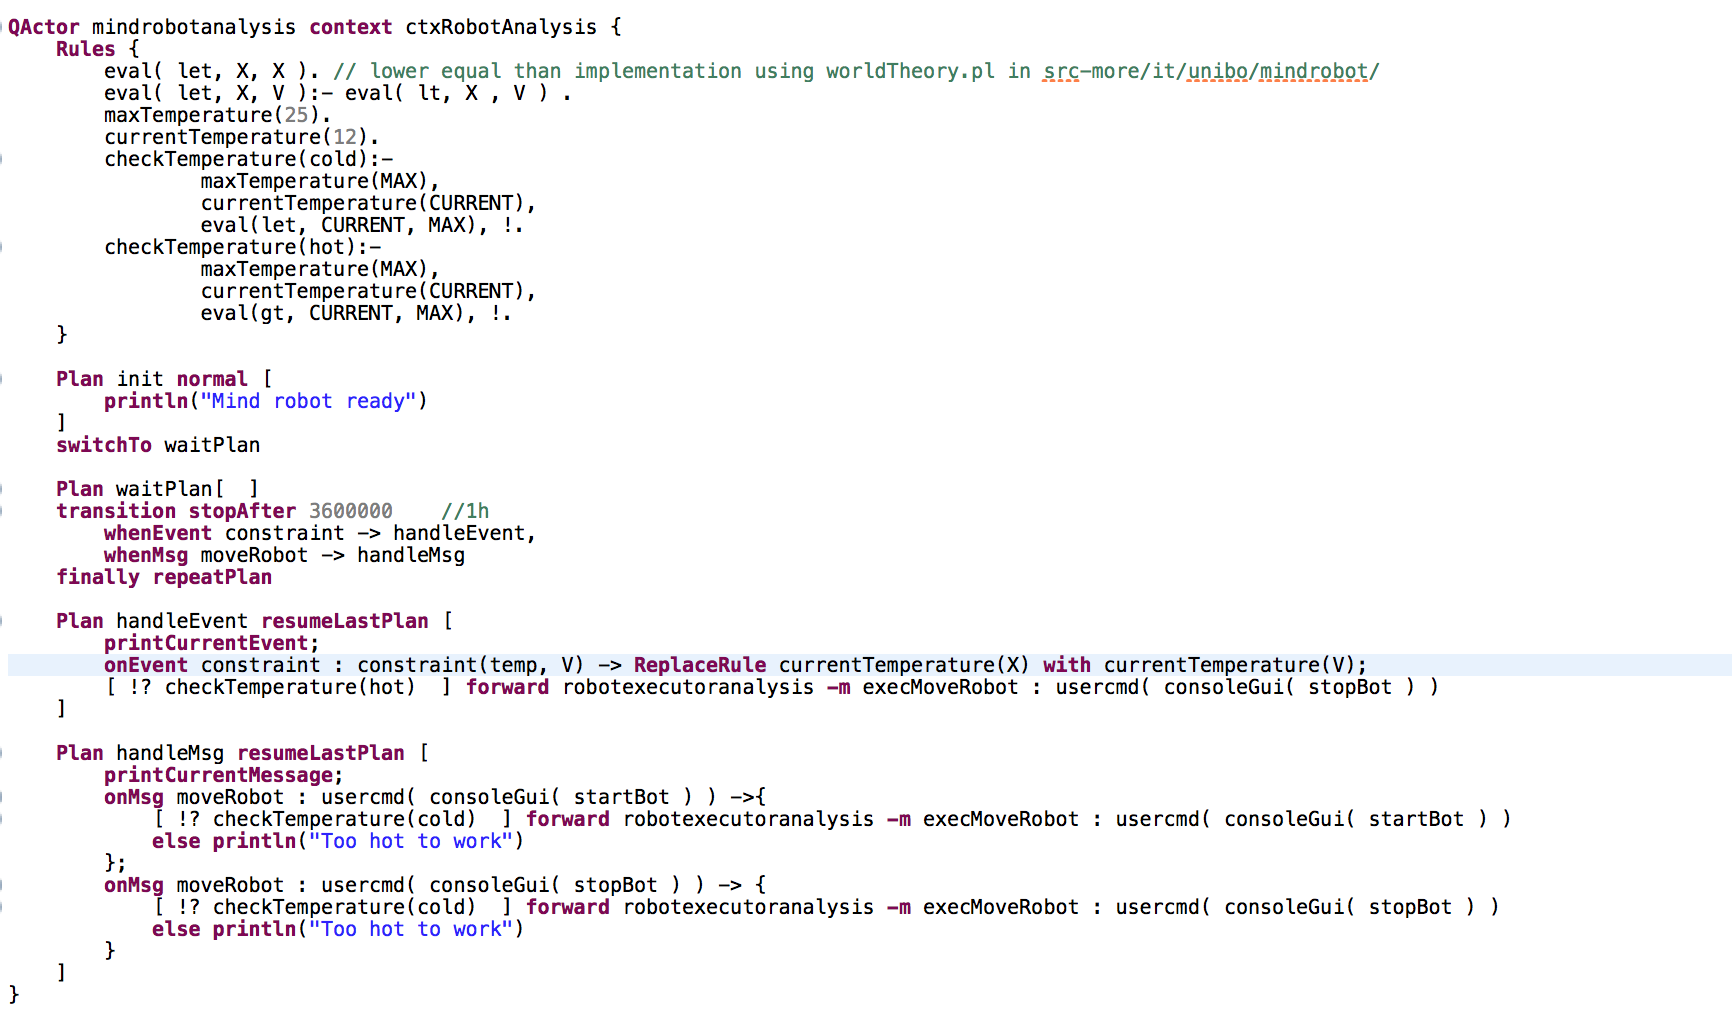
\includegraphics[width=1\textwidth]{Immagini/Requisito2/PAMind(Req2).png}
    \caption{Modello Mind Robot}
    \label{PAMindReq2}
\end{figure}
\vspace*{1ex}
\\
Nella base di conoscenza di questo modello viene introdotto il controllo del vincolo relativo alla temperatura, che abbiamo chiamato \textbf{checkTemperature(VALUE)}. Questo controllo restituir\`a un valore, \textit{True} o \textit{False}, in base al fatto che il vincolo sia soddisfatto o meno.\\
Come gi\`a analizzato in precedenza, in questo caso la console non comunicher\`a direttamente con il robot, ma piuttosto con la mind; sar\`a compito di quest'ultima controllare, prima di inoltrare il messaggio al robot, se la temperatura \`e al di sotto della soglia indicata. Da notare che nel modello \`e stato introdotto il seguente evento:\\
\begin{figure}
    \centering
    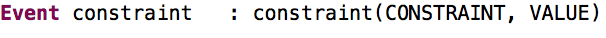
\includegraphics[width=1\textwidth]{Immagini/Requisito2/EventconstraintReq2.png}
    \caption{Event}
    \label{fig:EventReq2}
\end{figure}
\vspace*{1ex}
\\
Esso servir\`a per modificare il valore della temperatura, considerando il fatto che la temperatura di un luogo potrebbe cambiare.\\
La restante parte di modellazione \`e uguale a quella introdotta nell'analisi del problema del requisito 1 (\hyperref[AnalisidelproblemaReq1]{\ref{AnalisidelproblemaReq1}}). L'unica cosa che differisce dal caso precedente \`e il testing. Infatti in questo caso viene anche testato l'evento \textbf{constraint}, definito in precedenza, usato per modificare la base di conoscenza della mind. \\
\begin{figure}
    \centering
    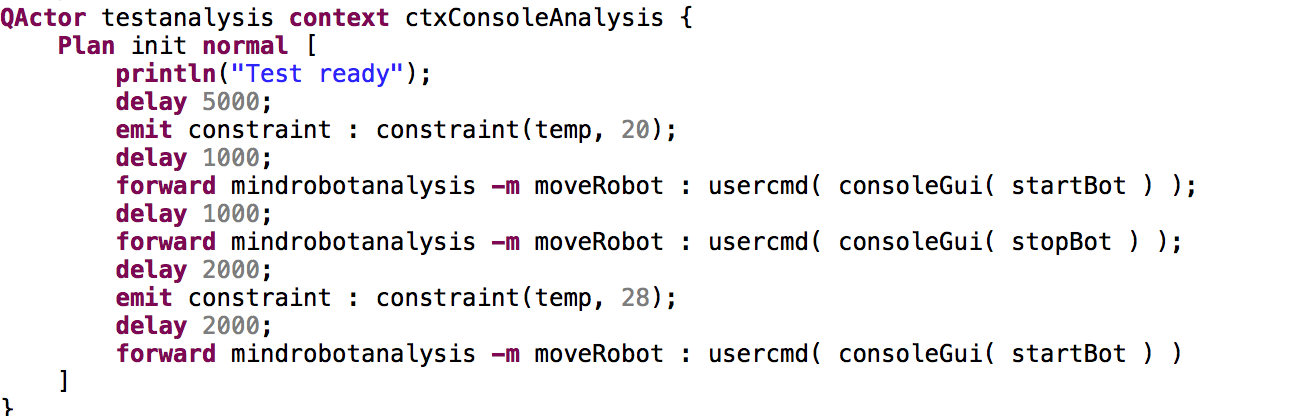
\includegraphics[width=1\textwidth]{Immagini/Requisito2/PATestReq2.png}
    \caption{Test analisi del problema}
    \label{fig:my_label}
\end{figure}
\vspace*{1ex}
\\
Il test in un primo caso porta la temperatura a 20 gradi Celsius - ancora valida, e in un secondo caso a 28 gradi Celsius - temperatura non pi\`u valida. Nel secondo caso il robot non dovr\`a muoversi.
Questo test ci ha dimostrato che l'interazione e il comportamento della mind funzionano come dovrebbero, quindi passiamo alla progettazione riprendendo le componenti introdotte nel requisito precedente.
\pagebreak 

%Requisito 2: Progettazione========================================================
\subsection{Progettazione}
\label{ProgettazioneReq2}
In fase di progettazione ci siamo accorti che la soluzione migliore, per rendere il sistema il pi\`u distribuito possibile, \`e definire un nuovo contesto solo per la \textbf{mind}. Questo ci permetter\`a di eseguire la mind in un qualsiasi nodo indipendente dai nodi del robot virtuale e del robot reale.\\
\begin{figure}
    \centering
    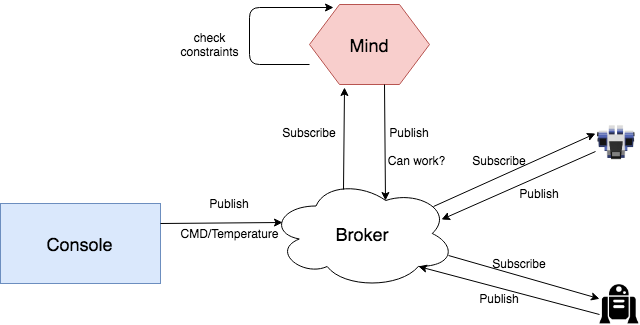
\includegraphics[width=1\textwidth]{Immagini/Requisito2/DiagrammaMind.png}
    \caption{Schema Mind}
    \label{PSchemaMind}
\end{figure}
\vspace*{1ex}
\\
Importante in questa fase \`e l'evento constraint che abbiamo introdotto nell'analisi del problema, in quanto permetter\`a di volta in volta di modificare la temperatura presente nella base di conoscenza della mind.\\
Rimane per\`o un problema:
\begin{itemize}
    \item Chi deve aggiornare la temperatura?
\end{itemize}
Dopo un attento studio e considerando i test effettuati nell'analisi del problema siamo arrivati alla conclusione che deve essere la console ad aggiornarla. In questo modo sulla console potr\`a essere visulizzata la temperatura relativa alla posizione del robot, in modo tale che anche l'utente autorizzato possa vederla.\\
Quindi, ripercorrendo quanto detto finora, i passi che saranno eseguiti per l'aggiornamento della temperatura sono i seguenti:
\begin{enumerate}
    \item La console stabilisce in base alla posizione del robot la temperatura: per rendere le cose pi\`u semplici abbiamo deciso che la posizione viene stabilita dall'utente attraverso un apposito campo del suo profilo;
    \item Ogni volta che la temperatura cambia viene inviata alla mind: per semplificare abbiamo deciso di aggiornare il valore della temperatura ogni 30 secondi;\label{secPuntoTemp}
    \item La mind valuta se la temperatura inviata \`e al di sotto della soglia indicata.
\end{enumerate}
Rimane ora il problema fondamentale sul come fare tutto ci\`o per realizzare un secondo prototipo da far visionare al committente; di questo ce ne occuperemo in fase di implementazione.

%Requisito 2: Implementazione========================================================
\subsection{Implementazione}
\label{ImplementazioneReq2}
Non verranno riportate le implementazioni del \textbf{Virtual Robot} e del \textbf{Real Robot} in quanto non sono state effettuate modifiche rispetto al requisito precedente.
% Implementazione: Mind ======================================================================
\subsubsection{Implementazione: Mind} .
\label{ImplementazioneReq2Mind}
\vspace*{1ex}
\\
Per realizzare la struttura individuata nella fase di progettazione abbiamo iniziato con l'implementazione del modello della mind. Visto che nell'analisi del problema era stato gi\`a definito un modello (Fig. \hyperref[PAMindReq2]{\ref{PAMindReq2}}) che ne raccogliesse le informazioni essenziali in ambiente locale, abbiamo adattato tale modello ad un ambiente distribuito.
\\
\begin{figure}
    \centering
    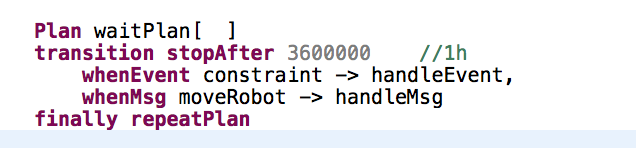
\includegraphics[width=0.6\textwidth]{Immagini/Requisito2/MsgReq2.png}
    \caption{Gestori}
    \label{fig:GestMind}
\end{figure}
In figura sono mostrati il \textbf{gestore degli eventi} e \textbf{il gestore dei messaggi}: il primo si occupa di gestire l'evento constraint ricevuto dalla console (\hyperref[fig:EventReq2]{\ref{fig:EventReq2}}), il secondo i messaggi relativi al movimento del robot.\\
Come avevamo gi\`a anticipato in fase di analisi e di progettazione, i messaggi (\texttt{moveRobot}) relativi ai comandi inviati dalla console verranno gestiti dalla mind. Questo ci permetter\`a di inviare il messaggio ai robot solo se sono soddisfatti i vincoli. Quindi, considerando la base di conoscenza definita in fase di analisi del problema (\hyperref[AnalisidelproblemaReq2Mind]{\ref{AnalisidelproblemaReq2Mind}}), il gestore dei messaggi diventer\`a quello mostrato nella figura che segue.\\
\begin{figure}
    \centering
    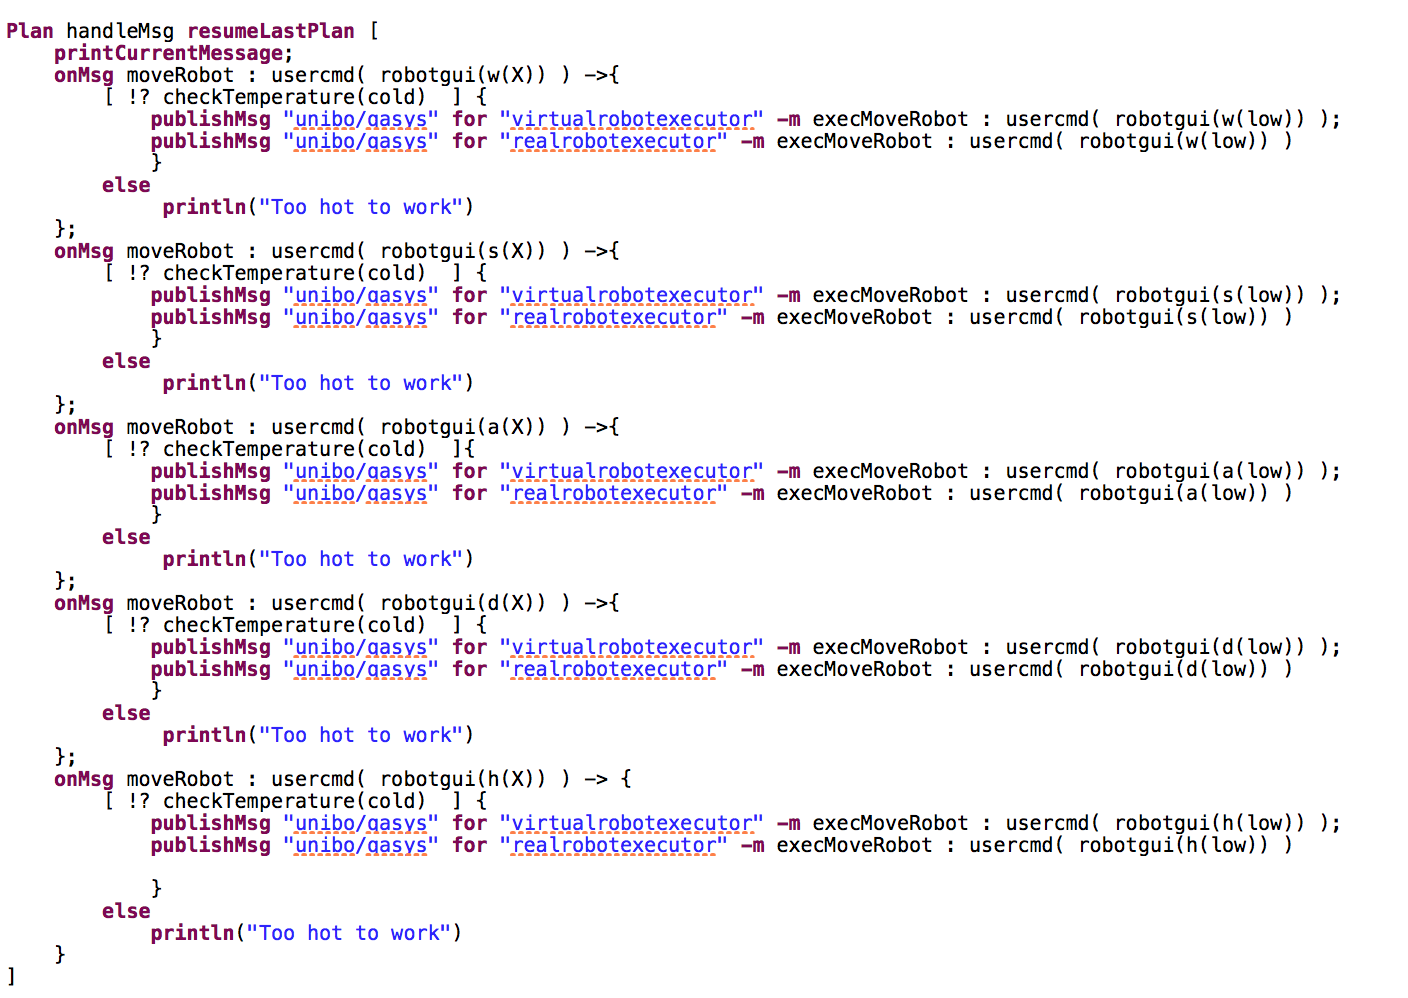
\includegraphics[width=1\textwidth]{Immagini/Requisito2/HandleMsgReq2.png}
    \caption{Mind: HandleMsg}
    \label{fig:MindHandleMsg}
\end{figure}
\vspace*{1ex}
\\
Nel codice sono state inserite delle \textbf{guardie} che verificano se una condizione \`e soddisfatta o meno.\\
\texttt{[ !? checkTemperature(cold)  ]}\\
Se la condizione \`e soddisfatta, allora la mind pubblica un messaggio su mqtt che indica ai robot il movimento da effettuare, altrimenti stampa la seguente stringa: "\textit{Too hot to work}".\\
Dal canto suo il \textbf{gestore dell'evento}, ogni volta che ricever\`a l'evento \textbf{constraint}, dovr\`a \textbf{aggiornare} la temperatura presente nella \textbf{base di conoscenza} e verificare se i vincoli sono rispettati. Nel caso in cui \textbf{non} lo siano deve inviare al robot un messaggio di Stop (sempre attraverso mqtt come nel caso precedente).\\
\begin{figure}
    \centering
    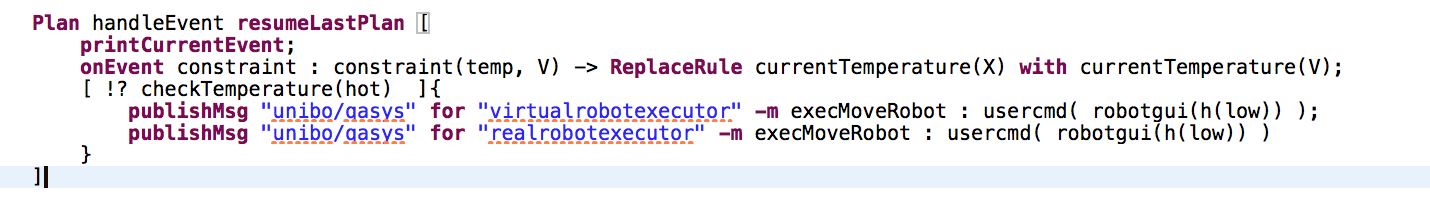
\includegraphics[width=1\textwidth]{Immagini/Requisito2/handleEvtReq2.png}
    \caption{Mind: HandleEvent}
    \label{fig:MindHandleEvent}
\end{figure}

% Implementazione: Aggiornamento Console ======================================================================
\subsubsection{Implementazione: Aggiornamento Console} .
\label{ImplementazioneReq2Console}
\vspace*{1ex}
\\
La console, a fronte delle considerazioni fatte nei paragrafi precedenti, subir\`a delle leggere modifiche.
Infatti ora dovr\`a anche ricavare la temperatura relativa alla posizione del robot; come gi\`a detto in fase di progettazione, per la \textbf{posizione} del robot ci baseremo su un campo inserito dall'utente durante la registrazione. Per ricavare la temperatura, invece, viene usata un'apposita \textbf{API}(Fig. \hyperref[fig:MindHandleEvent]{\ref{fig:MindHandleEvent})}.\\
\begin{figure}
    \centering
    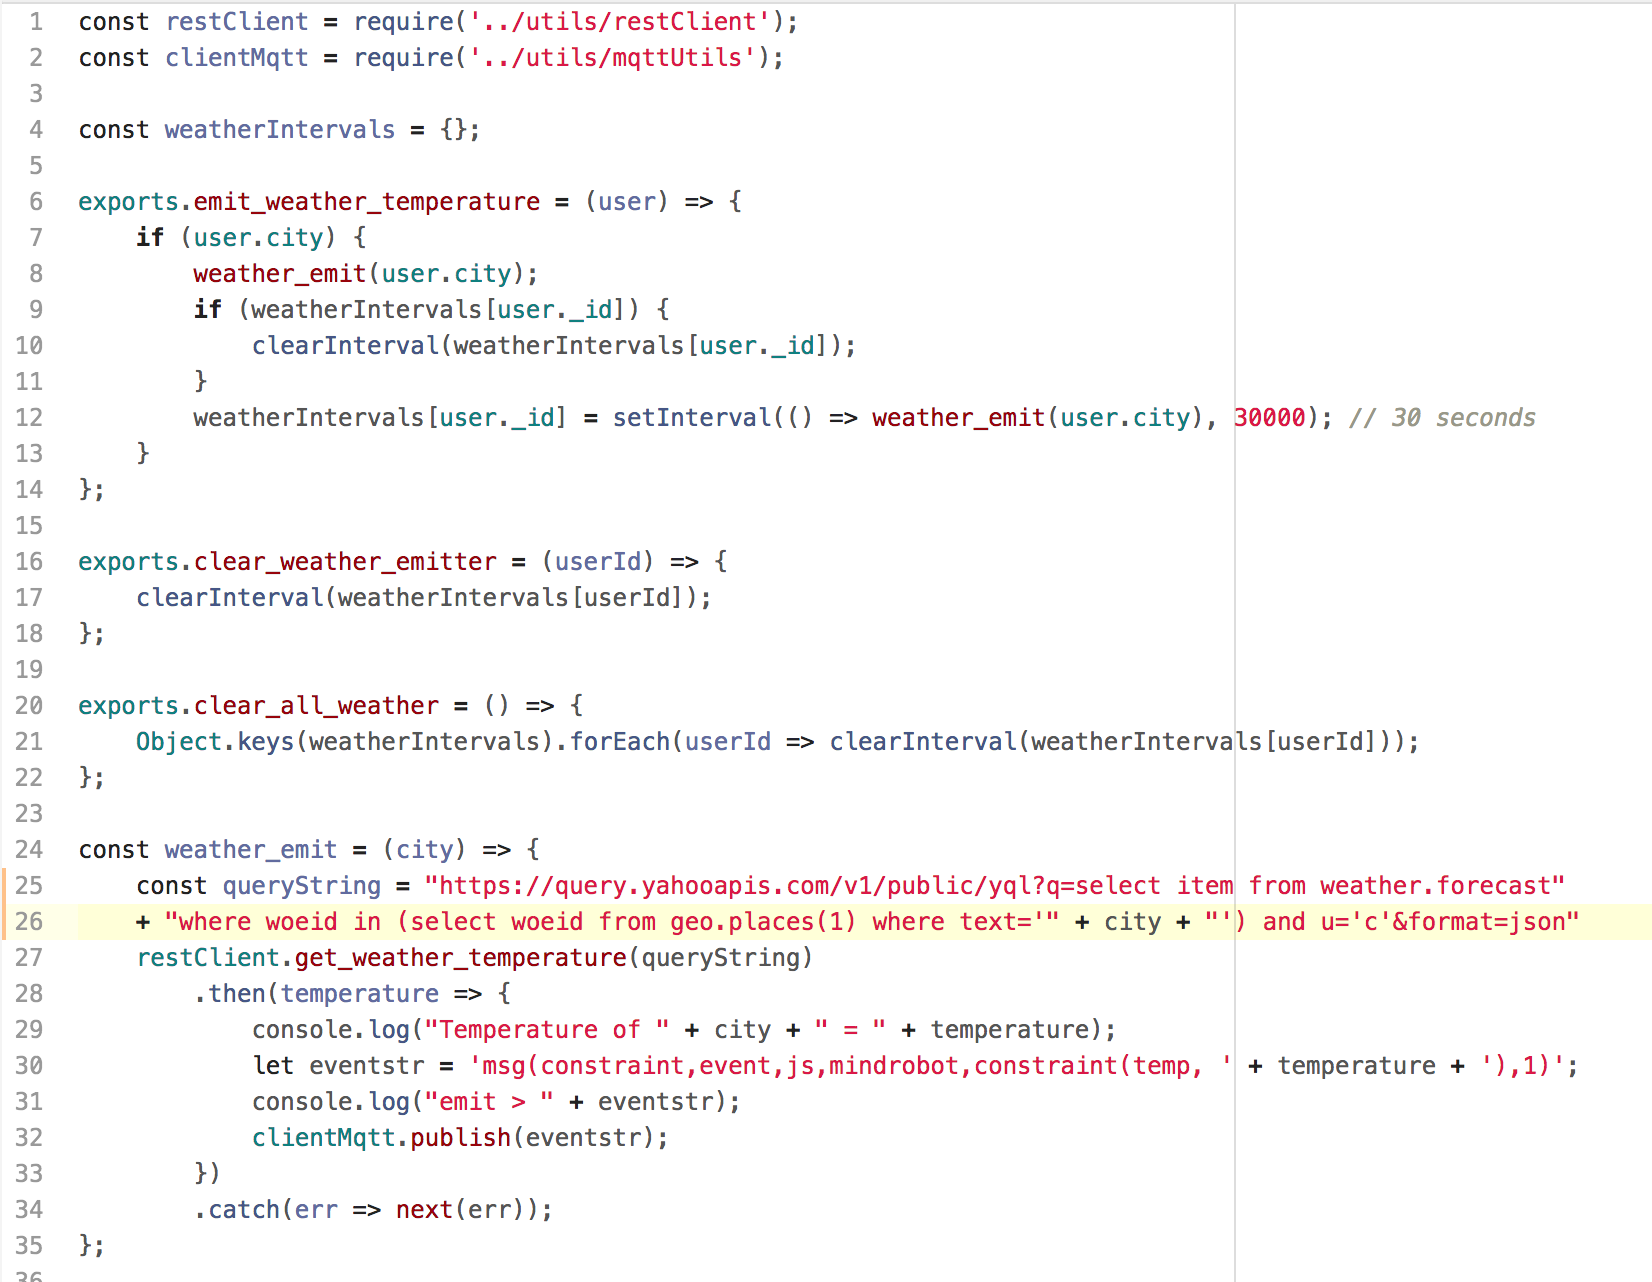
\includegraphics[width=1\textwidth]{Immagini/Requisito2/TemperatureAPI.png}
    \caption{API Temperatura}
    \label{fig:MindHandleEvent}
\end{figure}
Come stabilito in fase di progettazione, verr\`a emesso un evento ogni \textbf{30} secondi che conterr\`a il valore della temperatura relativa alla posizione stabilita dall'utente autorizzato in fase di registrazione.\\
\begin{figure}
    \centering
    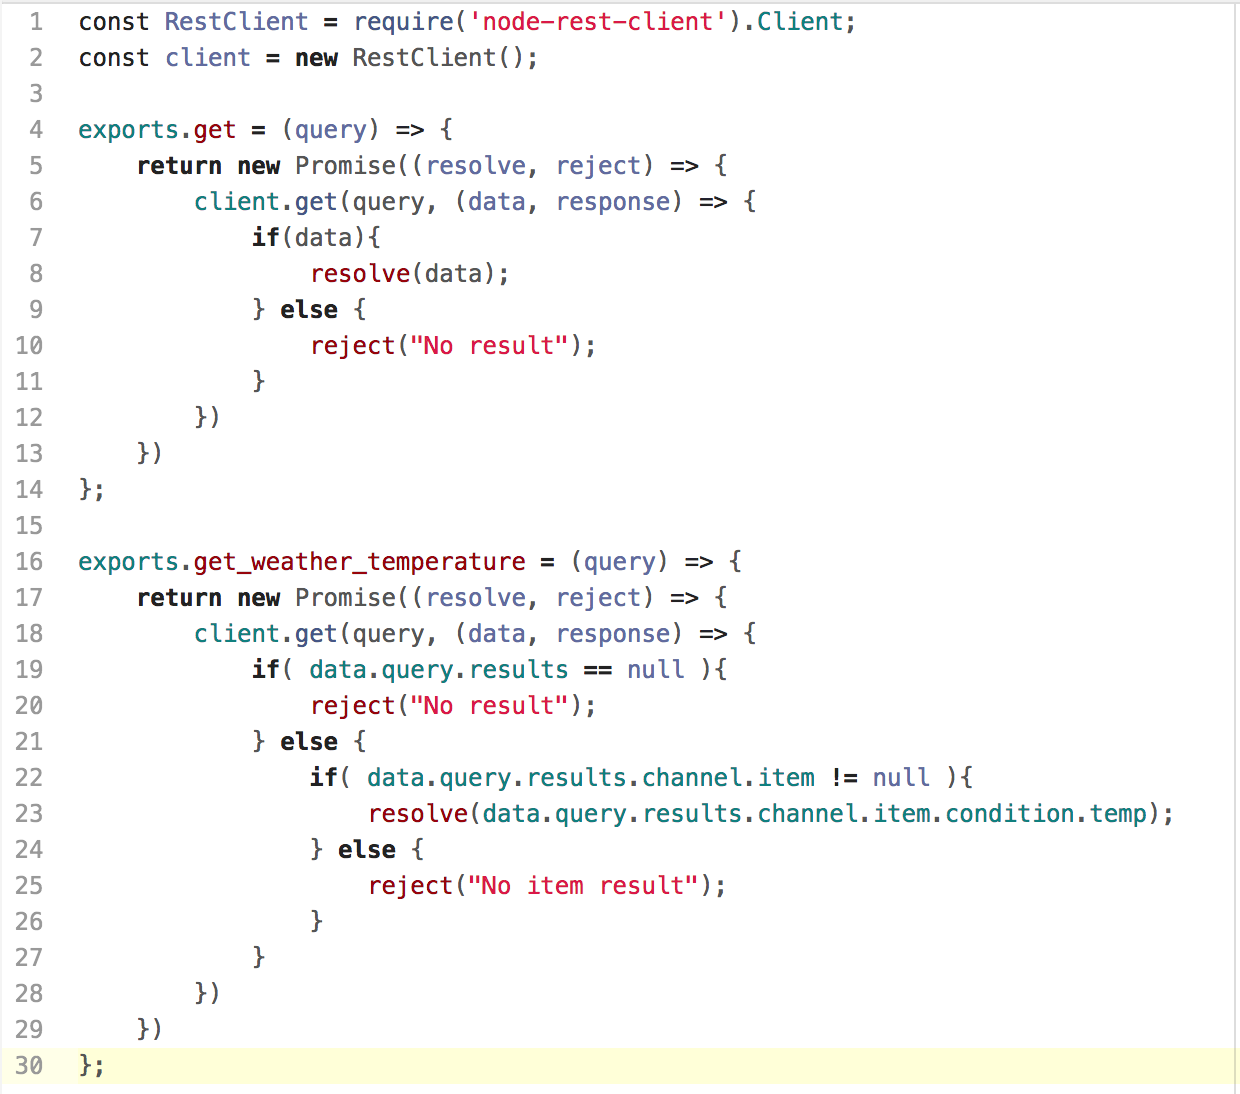
\includegraphics[width=1\textwidth]{Immagini/Requisito2/clientRestReq2.png}
    \caption{ClientRest}
    \label{fig:ClientRestReq2}
\end{figure}
\vspace*{1ex}
\\
In Fig. \hyperref[fig:ClientRestReq2]{\ref{fig:ClientRestReq2}} viene riportato il clientRest, ovvero colui che effettuar\`a la vera e propria chiamata \textbf{REST} al link \texttt{https://query.yahooapis.com}, per ottenere la temperatura.\\

A questo punto non ci restava altro che mostrare la temperatura direttamente sulla console dell'utente autenticato. Per farlo \`e bastato aggiornare la componente \textbf{Console.js} di React. Il risultato finale a livello grafico \`e quello mostrato in figura.\\
\begin{figure}
    \centering
    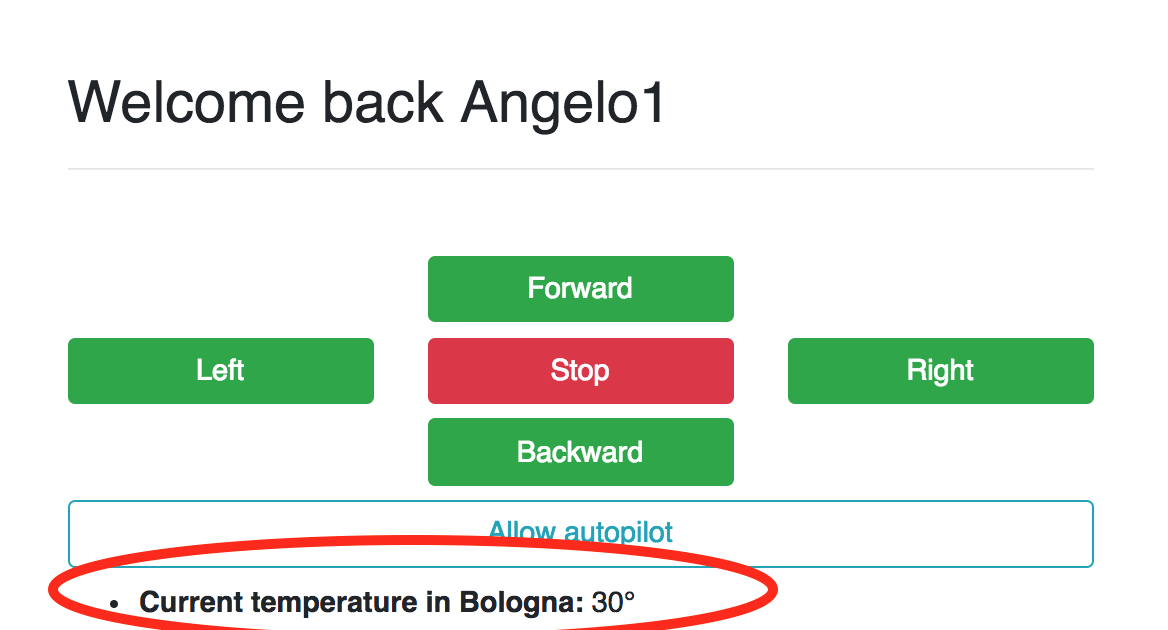
\includegraphics[width=0.6\textwidth]{Immagini/Requisito2/ConsoleReq2(1).png}
    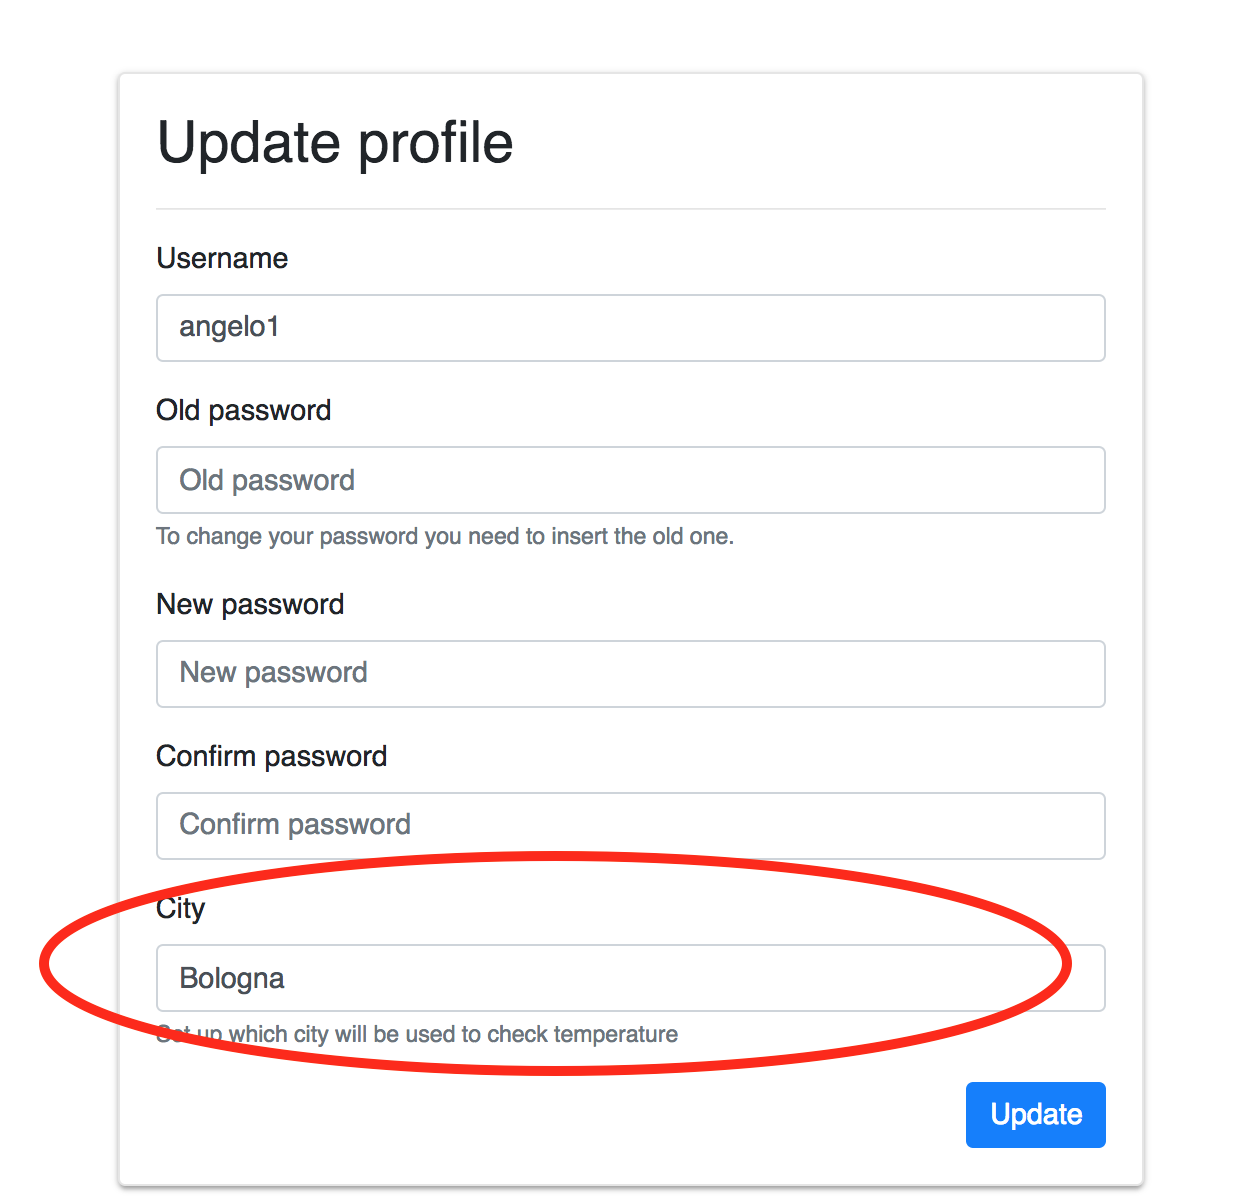
\includegraphics[width=0.3\textwidth]{Immagini/Requisito2/ConsoleReq2(2).png}
    \caption{Console aggiornata}
    \label{fig:ConsoleUpdateReq2}
\end{figure}
\vspace*{1ex}
\\
Per effettuare altri test, come si pu\`o notare dalla figura, \`e possibile modificare la citt\`a anche una volta che l'utente si \`e registrato direttamente dalla pagina della console.\\
Degno di nota \`e il fatto che la pubblicazione dell'evento constraint su mqtt viene fatto di volta in volta dal web server presente nella console.\\
\textbf{Arrivati a questo punto possiamo presentare un altro prototipo funzionante al commitente}, che soddisfa il secondo requisito.
\pagebreak

%=Requisito 3===============================================================
%R-TimeOk: the current clock time is within a given interval (e.g. between 7 a.m and 10 a.m ).
\section{Requisito 3}
\label{Requisito3}
%Requisito 3: Analisi del problema ==========================================================
\subsection{Analisi del problema}
\label{AnalisidelproblemaReq3}
Dall'analisi dei requisiti si deduce che occorre introdurre un nuovo vincolo: \textit{se l'orario corrente non \`e compreso all'interno di un intervallo (ad esempio non \`e tra le 7 e le 10 di mattina) il robot deve fermare la sua attivit\`a}. Da qui si capisce bene come il fatto di aver introdotto un componente (\textbf{mind}) che si occupi del controllo del rispetto dei vincoli sia la scelta migliore.\\ Dopo l'interazione con l'utente in fase di analisi dei requisiti si \`e stabilito che l'orario deve essere \textbf{newtoniano} e relativo al \textbf{fuso orario} del \textbf{robot}. Quindi la scelta pi\`u conveniente sar\`a quella di far stabilire l'orario del robot alla mind e di volta in volta inviarlo alla console, in modo tale che anche l'utente autorizzato possa visionarlo. %Di quest'ultimo caso ce ne preoccuperemo in fase di progettazione, ora ci occuperemo dell'aggiornamento della base di conoscenza della \textbf{mind}.\\

% Analisi del problema 3: Mind ======================================================================
\subsubsection{Analisi del problema: Mind} .
\label{AnalisidelproblemaReq3Mind}
\vspace*{1ex}
\\
Alla nostra base di conoscenza andiamo ad introdurre una nuova regola che controlli che il nuovo vincolo sia rispettato. Bisogna anche tenere in considerazione che, allo stesso tempo, anche il vincolo della temperatura deve essere soddisfatto.\\
Quindi partendo dalla base di conoscenza introdotta in precedenza (\hyperref[AnalisidelproblemaReq2Mind]{\ref{AnalisidelproblemaReq2Mind}}), introduciamo le seguenti regole:\\
\begin{figure}
    \centering
    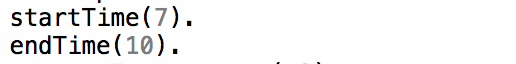
\includegraphics[width=0.5\textwidth]{Immagini/Requisito3/StartEndReq3.png}
    \caption{Intervallo di tempo (anche se non riportata in figura ci sar\`a una regola \textbf{currentTime} che indica l'ora corrente)}
    \label{fig:my_label}
\end{figure}
\vspace*{1ex}
\\
Tali regole ci permettono di stabilire l'intervallo di tempo in cui il robot pu\`o svolgere la sua attivit\`a. Per controllare, invece, che questo intervallo venga rispettato bisogna introdurre un'ulteriore regola, mostrata nella figura \hyperref[fig:checkTime]{\ref{fig:checkTime}}. \\
\begin{figure}
    \centering
    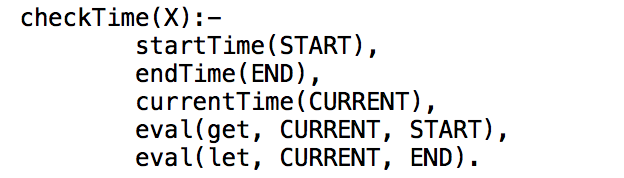
\includegraphics[width=0.7\textwidth]{Immagini/Requisito3/checkTimeReq3.png}
    \caption{Controllo del vincolo}
    \label{fig:checkTime}
\end{figure}
\vspace*{1ex}
\\
L'unica cosa che rimane da fare prima di testare se la base di conoscenza funziona correttamente \`e controllare che anche il vincolo della temperatura sia soddisfatto. Per farlo viene introdotta un'ultima regola illustrata nella figura \hyperref[fig:checkConstraint]{\ref{fig:checkConstraint}}.\\
\begin{figure}
    \centering
    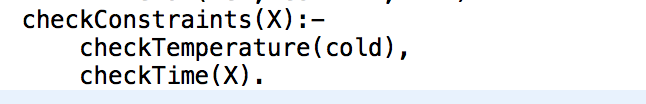
\includegraphics[width=0.7\textwidth]{Immagini/Requisito3/CheckConstraintReq3.png}
    \caption{Controllo dei vincoli}
    \label{fig:checkConstraint}
\end{figure}
\vspace*{1ex}
\\
Per testare che la base di conoscenza funzioni, utilizziamo l'evento  definito in precedenza(Fig. \hyperref[fig:EventReq2]{\ref{fig:EventReq2}}) per aggiornare l'orario ad un orario non valido.\\
\begin{figure}
    \centering
    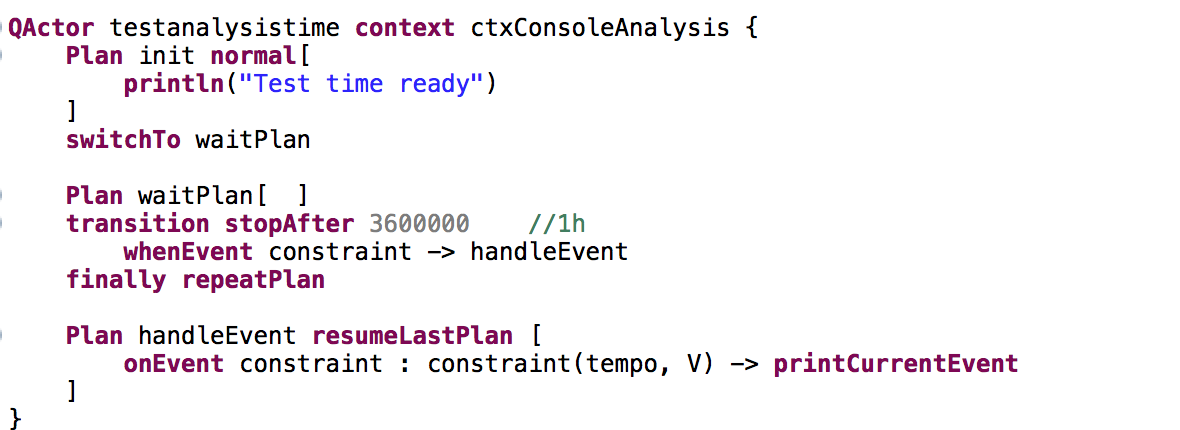
\includegraphics[width=0.8\textwidth]{Immagini/Requisito3/TestReq3.png}
    \caption{Test del requisito 3}
    \label{fig:TestReq3}
\end{figure}
\vspace*{1ex}
\\
Il test (Fig. \hyperref[fig:TestReq3]{\ref{fig:TestReq3}}) ha avuto esito positivo, quindi siamo certi che la base di conoscenza abbia il comportamento aspettato.\\
Dopo aver stabilito \textbf{come} effettuare i controlli, usando il modello della mind definito nel requisito 2 con la base di conoscenza appena ridefinita, vedremo in fase di progettazione come mettere tutto insieme.

%Requisito 3: Progettazione========================================================
\subsection{Progettazione}
\label{ProgettazioneReq3}
In fase di progettazione andremo a stabilire come ottenere l'orario corrente e come comunicarlo al sistema. Per ottenere l'orario abbiamo deciso di utilizzare un metodo statico che vada a ricavare l'ora corrente e che aggiorni la base di conoscenza della \textbf{mind}. Una volta che la mind avr\`a usato questo metodo, andr\`a a comunicare il risultato ottenuto alla console, attraverso il modello publish/subscribe che caratterizza il nostro sistema.\\
Il metodo statico che andremo a definire in fase di implementazione dovr\`a essere richiamato ogni volta che la console invia un comando da eseguire, in modo tale che la mind, prima di verificare che l'orario rispetti il vincolo, possa averlo sempre aggiornato. \\
\begin{figure}
    \centering
    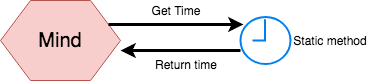
\includegraphics[width=0.8\textwidth]{Immagini/Requisito3/MindReq3.png}
    \caption{Schema richiesta dell'orario}
    \label{fig:TestReq3}
\end{figure}
\vspace*{1ex}
\\

%Requisito 3: Implementazione========================================================
\subsection{Implementazione}
\label{ImplementazioneReq3}
% Implementazione: Metodo Statico ======================================================================
\subsubsection{Implementazione: Metodo Statico} .
\label{ImplementazioneReq3MetodoStatico}
\vspace*{1ex}
\\
Il metodo statico dovr\`a ricavare l'orario corrente e per farlo user\`a la classe \texttt{Date} di \java, in particolare per avere il formato adatto dell'ora:\\
\begin{verbatim}
SimpleDateFormat sdf = new SimpleDateFormat("HH");
String hours = sdf.format(new Date());
\end{verbatim}
Una volta ottenuto l'orario, dovr\`a aggiornare la base di conoscenza della \textbf{mind}. Per poter modificare la base di conoscenza dovr\`a avere accesso ai metodi del \textbf{\qa}.\\
Una volta che si ha il \qa si potr\`a accedere alla base di conoscenza e aggiornare l'orario corrente:
\begin{verbatim}
    myActor.replaceRule("currentTime(X)", "currentTime("+hours+")");
\end{verbatim}
La definizione del metodo sar\`a quindi la seguente:
\begin{verbatim}
    //myActor corrisponde al \qa che ha invocato il metodo
    public static void getHours(QActor myActor) 
\end{verbatim}
\pagebreak
% Implementazione: Mind ======================================================================
\subsubsection{Implementazione: Mind} .
\label{ImplementazioneReq3Mind}
\vspace*{1ex}
\\
La Mind, arrivati a questo punto dell'implementazione, dovr\`a aggiornare l'ora ogni volta che riceve un comando dalla console. Sar\`a quindi necessario apportare una modifica al gestore dei messaggi (Fig. \hyperref[fig:MindHandleMsg]{\ref{fig:MindHandleMsg}}).
\begin{figure}
    \centering
    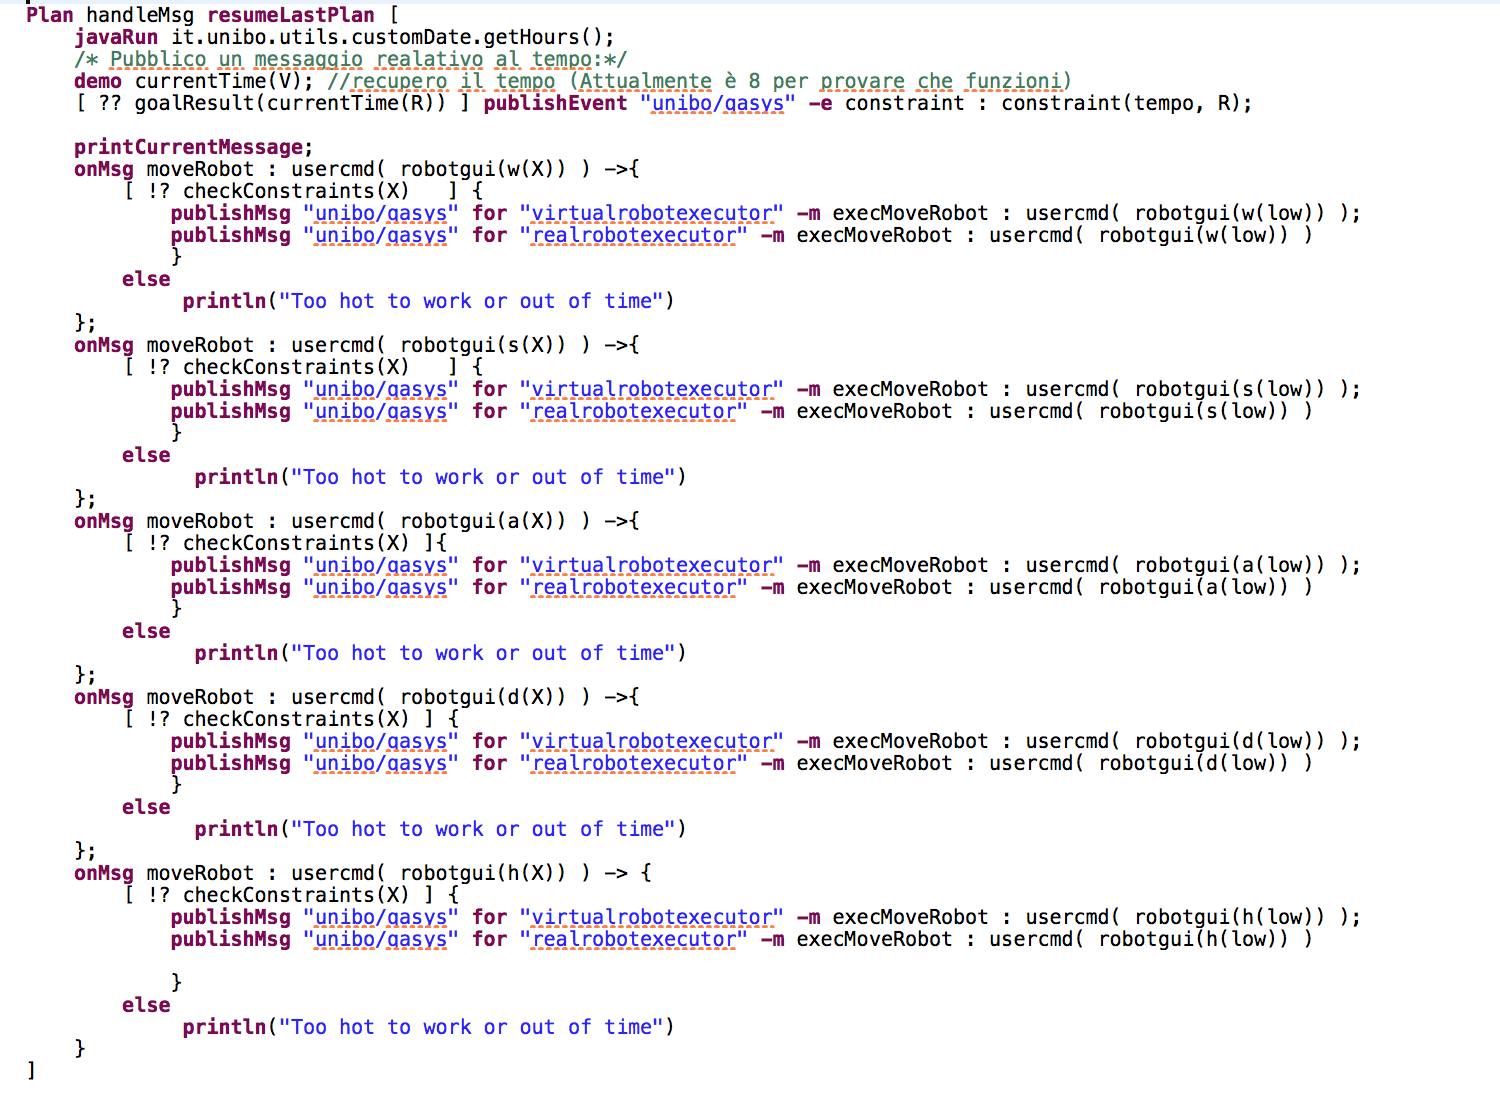
\includegraphics[width=1.3\textwidth]{Immagini/Requisito3/handleMsgReq3.png}
    \caption{Gestore messaggi}
    \label{fig:handleMsgReq3}
\end{figure}
Da notare che per ogni richiesta di movimento da parte della console si va a controllare che il predicato \textbf{checkConstraints} (definito nella Fig. \hyperref[fig:checkConstraint]{\ref{fig:checkConstraint}})  restituisca true e solo in quel caso si inoltra il messaggio ai robot. Inoltre, la mind dovr\`a aggiornare il sistema notificando l'ora appena ricevuta.
\begin{verbatim}
[ ?? goalResult(currentTime(R)) ] 
    publishEvent "unibo/qasys" -e constraint : constraint(tempo, R);
\end{verbatim}
\pagebreak
%=Requisito 4===============================================================
%While the robot is working:–it must blink a Led put on it, if the robot is a real robot (R-BlinkLed).–it must blink a Led Hue Lamp available in the house, if the robot is avirtual robot (R-BlinkHue).–it must avoid fixed obstacles (e.g. furniture) present in the room(R-AvoidFix)  and/or  mobile  obstacles  like  balls,  cats,  etc.  (R-AvoidMobile).
\section{Requisito 4}
\label{Requisito4}
%Requisito 4: Analisi del problema ==========================================================
\subsection{Analisi del problema}
\label{AnalisidelproblemaReq4}
La scelta fatta dopo aver analizzato questo requisito \`e stata quella di dividerlo in due parti: una prima parte che si concentra principalmente sul led e una seconda parte incentrata sugli ostacoli da evitare presenti nella stanza.\\
In questo capitolo ci occuperemo soltanto della prima parte, senza fare distinzione, in fase di analisi, tra il \textbf{led} e il \textbf{Led Hue Lamp} presente all'interno della casa.\\
Anche in questo caso la \textbf{mind} avr\`a un ruolo fondamentale, in quanto dovr\`a segnalare al led se il robot \`e in movimento o \`e fermo, in modo tale che possa stabilire se lampeggiare o meno.\\
Prima di vedere come realizzare l'interazione tra il led e la mind, cerchiamo di realizzare un modello del led che catturi gli aspetti essenziali del suo comportamento.

% Analisi del problema 4: Led Prima Versione ======================================================================
\subsubsection{Analisi del problema: Led Prima Versione} 
\label{AnalisidelproblemaReq4LedV1}
\vspace*{1ex}
\\
In questa prima versione del led, per la realizzazione del modello, useremo il linguaggio custom \qa, in quanto con questo potremo realizzare un attore che lavora in un contesto differente e quindi simulare il fatto che il led possa trovarsi in un nodo indipendente da quello della mind. In particolare l'attore rappresentante il led effettuer\`a una stampa della stringa: \textit{"Led blink"} se il robot \`e in movimento e \textit{"Led not blink"} se il robot \`e fermo (Fig. \hyperref[fig:ledModel]{\ref{fig:ledModel}}) .\\
\begin{figure}
    \centering
    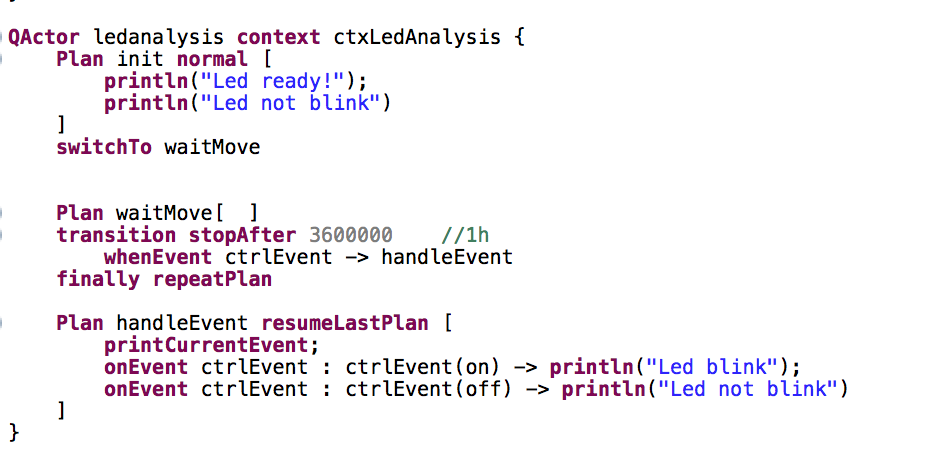
\includegraphics[width=1\textwidth]{Immagini/Requisito4/ledAnReq4.png}
    \caption{Modello Led}
    \label{fig:ledModel}
\end{figure}\\
L'evento \texttt{Event ctrlEvent : ctrlEvent(CMD)} verr\`a emesso dalla mind per segnalare che il robot \`e in movimento (Fig. \hyperref[fig:Req4AnMind]{\ref{fig:Req4AnMind}}).\\
\begin{figure}
    \centering
    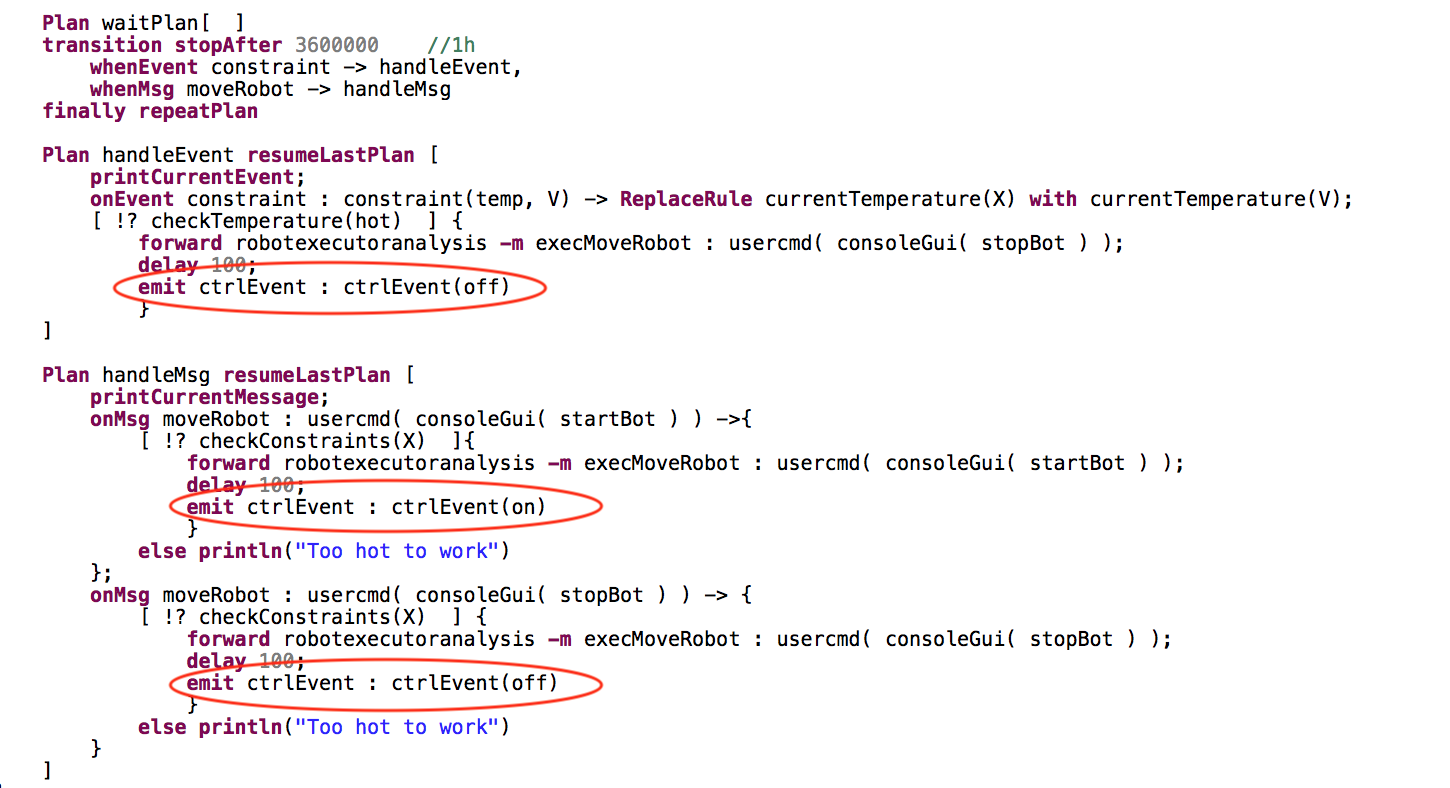
\includegraphics[width=1\textwidth]{Immagini/Requisito4/AnMindReq4.png}
    \caption{Analisi del problema: mind}
    \label{fig:Req4AnMind}
\end{figure}\\
A questo punto possiamo effettuare il test sull'interazione tra mind e led. Per farlo, come gi\`a fatto nei casi precedenti, basta simulare l'invio dei comandi da parte di una console (Fig. \hyperref[fig:testReq4]{\ref{fig:testReq4}}).\\
\begin{figure}
    \centering
    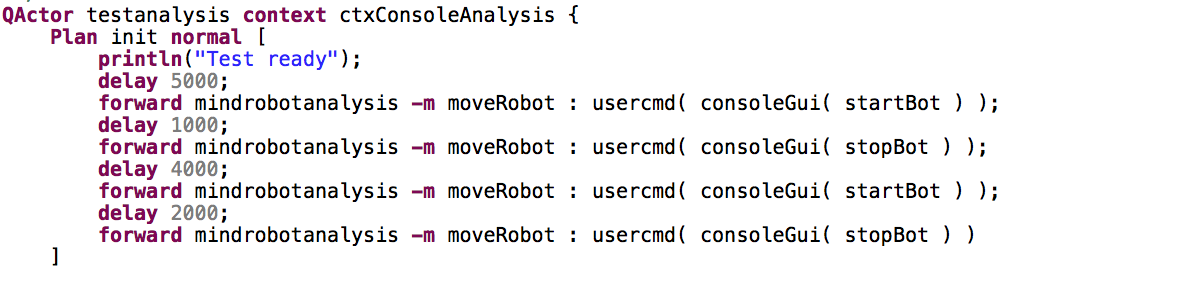
\includegraphics[width=1\textwidth]{Immagini/Requisito4/TestReq4.png}
    \caption{Test interazione}
    \label{fig:testReq4}
\end{figure}

% Analisi del problema 4: Led Prima Versione ======================================================================
\subsubsection{Analisi del problema: Led Seconda Versione} .
\label{AnalisidelproblemaReq4LedV2}
\vspace*{1ex}
\\
Per simulare il comportamento del led useremo un oggetto Mock (realizzato in \java) fornitoci dalla software house. In particolare:
\begin{itemize}
    \item se il led \`e spento l'oggetto Mock avvier\`a una piccola Gui di colore rosso;
    \item se il led \`e acceso l'oggetto Mock avvier\`a una Gui pi\`u grande rispetto alla precedente.
\end{itemize}
L'oggetto Mock inoltre espone un metodo che permetter\`a di avere un alternarsi tra interfaccia grande e interfaccia piccola, in pratica ci permette di simulare il "lampeggiare" del nostro led.\\
Il modello del led, dopo l'introduzione dell'oggetto Mock, sar\`a quello mostrato in figura \hyperref[fig:ledMockobj]{\ref{fig:ledMockobj}}.\\
\begin{figure}
    \centering
    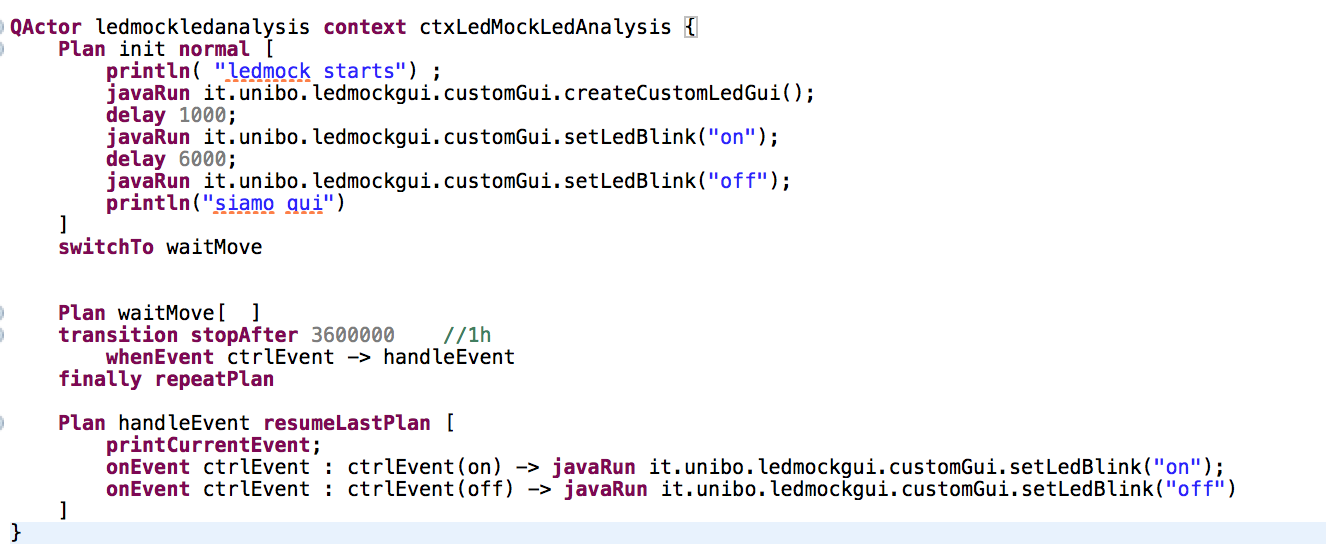
\includegraphics[width=1\textwidth]{Immagini/Requisito4/LedMockReq4.png}
    \caption{Modello Led con l'utilizzo dell'oggetto Mock}
    \label{fig:ledMockobj}
\end{figure}
\vspace*{1ex}
\\
Il test \`e identico a quello precedente; la differenza sta nel fatto che mentre prima avevamo una semplice stampa ora abbiamo una vera e propria simulazione del comportamento del led.
\clearpage

%Requisito 4: Progettazione ==========================================================
\subsection{Progettazione}
\label{ProgettazioneReq4}
In fase di progettazione andiamo a sostituire il \qa aggiunto in fase di analisi con un ulteriore componente per separare le parti gi\`a esistenti da quella che si occupa della gestione del led, in quanto, d'ora in avanti, si avr\`a una distinzione tra il \textbf{led fisico} sul real robot e il \textbf{led hue lamp} sul virtual robot.\\
Questo nuovo componente verr\`a realizzato cercando di ottenere una struttura generale ed indipendente, utilizzabile per entrambe le tipologie di led e facilmente estendibile in futuro.\\
\begin{figure}
    \centering
    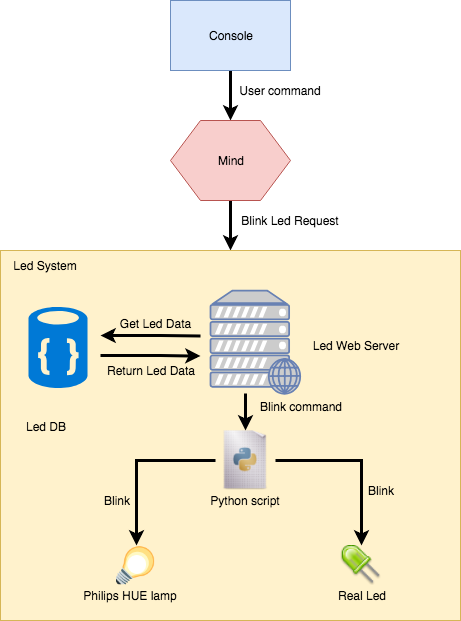
\includegraphics[width=0.7\textwidth]{Immagini/Requisito4/Req4MindWithServerLamp.png}
    \caption{Sistema led}
    \label{fig:ledSystemReq4}
\end{figure}
\vspace*{1ex}
\\
Come si pu\`o notare dalla figura (\hyperref[fig:ledSystemReq4]{\ref{fig:ledSystemReq4}}) questo sistema si compone principalmente di: 
\begin{itemize}
    \item un \textbf{web server} (scritto in NodeJS) che avr\`a il compito di comunicare tramite chiamate HTTP con la mind;
    \item Di un \textbf{database} (MongoDB) in cui saranno salvate le informazioni relative ai led presenti nel sistema;
    \item Di uno \textbf{script python} in grado di comunicare tramite socket con il web server e che avr\`a il compito di far accendere i led.
\end{itemize}

%Requisito 4: Implementazione ==========================================================
\subsection{Implementazione}
\label{ImplementazioneReq4}

% Implementazione: Client Rest ======================================================================
\subsubsection{Implementazione: Client Rest} .
\label{ImplementazioneReq4ClientRest}
\vspace*{1ex}
\\
L'implementazione di questo requisito ha richiesto una modifica nella mind; infatti \`e stato eliminato l'evento introdotto in fase di analisi del problema (\texttt{Event ctrlEvent : ctrlEvent(CMD)}). Al suo posto \`e stata inserita una chiamata HTTP realizzata mediante un metodo statico custom creato appositamente per questa funzione (il \textbf{Client Rest}). \\
Questo metodo prende in ingresso 3 parametri:
\begin{itemize}
    \item Il comando da inviare al web server dei led (\textbf{true} per far blinkare il led e \textbf{false} per farlo smettere);
    \item L'eventuale colore del led nel caso del Led Hue;
    \item L'uri da utilizzare per effettuare la chiamata HTTP.
\end{itemize}\\
\begin{figure}
    \centering
    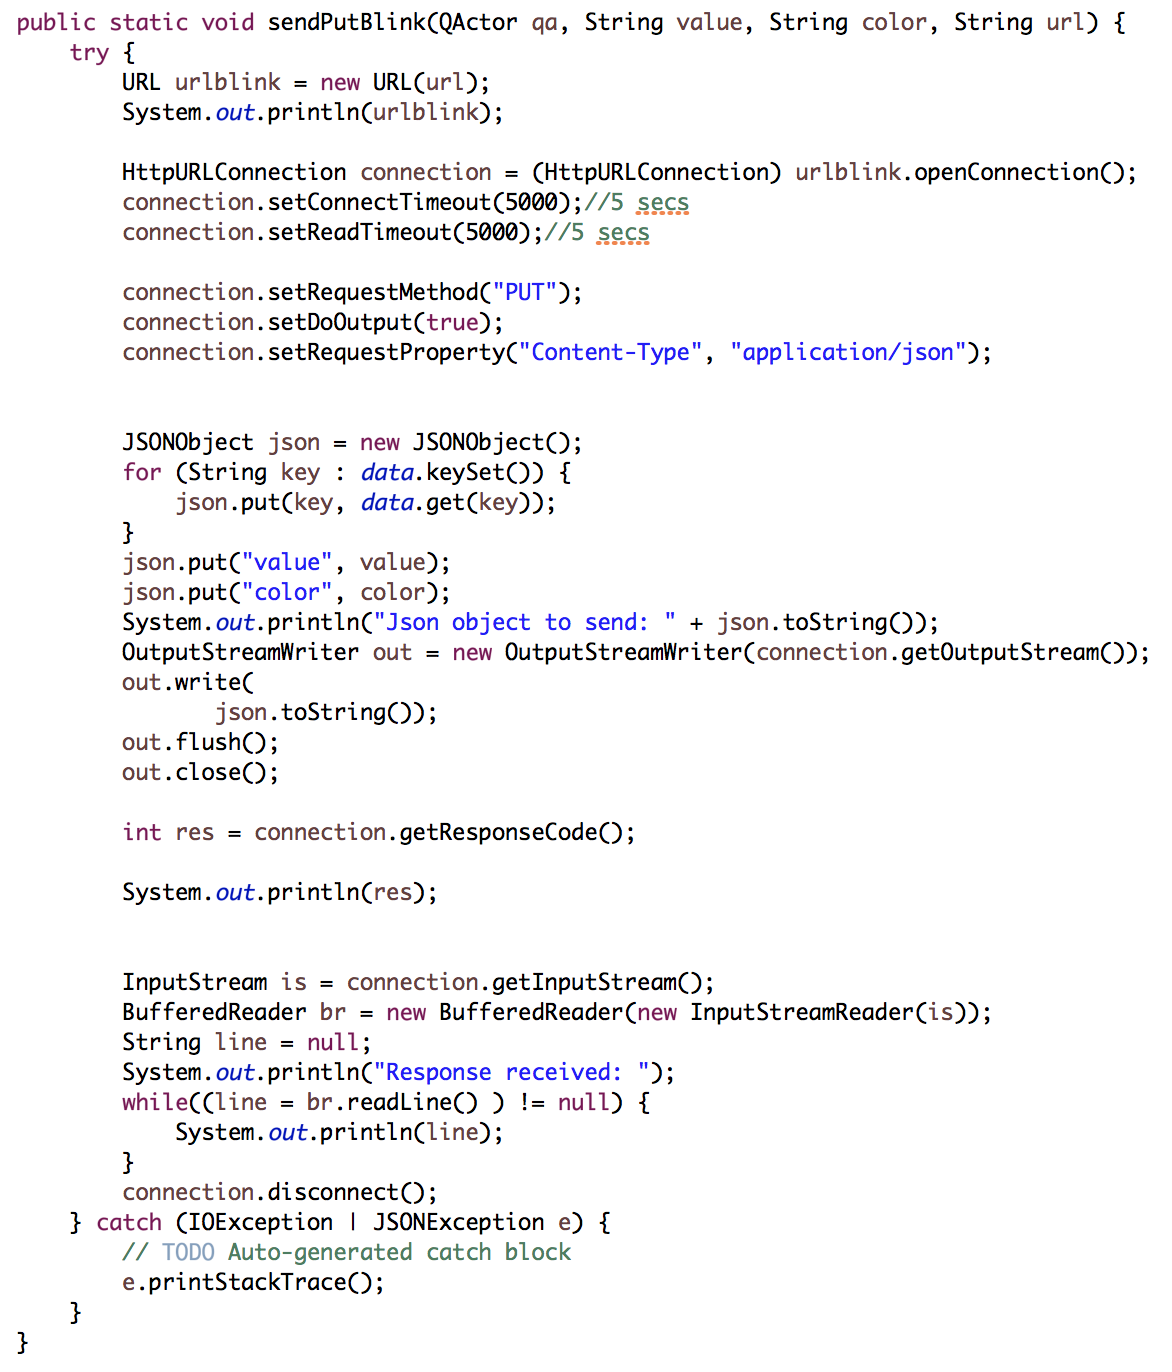
\includegraphics[width=1\textwidth]{Immagini/Requisito4/ClientRest.png}
    \caption{Codice del metodo statico per la chiamata HTTP}
    \label{fig:CodeClientRestReq4}
\end{figure}
\vspace*{1ex}
\pagebreak
\\
Il metodo, come si evince dalla figura (\hyperref[fig:CodeClientRestReq4]{\ref{fig:CodeClientRestReq4}}), prepara una chiamata PUT al web server dei led, crea un JSON Object in cui va ad inserire il body della chiamata (ovvero due parametri value e color) ed infine invia la richiesta HTTP e stampa la risposta ricevuta dal server.
% Implementazione: Led System ======================================================================
\subsubsection{Implementazione: Led System} .
\label{ImplementazioneReq4LedSystem}
\vspace*{1ex}
\\
Nell'implementazione di questo componente ci siamo concentrati inizialmente nella realizzazione del web server e dello script python. Infine sono stati creati all'interno dello script python degli adapter specifici per le due tipologie di led necessarie.

% Implementazione: Web Server ======================================================================
\subsubsection{Implementazione: Web Server} .
\label{ImplementazioneReq4WebServer}
\vspace*{1ex}
\\
Il Web Server, ogni volta che ricever\`a una richiesta dalla mind, dovr\`a inviare sulla socket stabilita con lo script python il comando richiesto. In tale richiesta, oltre alla specifica del \textbf{comando}, possono essere presenti:
\begin{itemize}
    \item il \textbf{codice univoco} della lampadina sulla quale attuare il comando (\textbf{obbligatorio});
    \item il \textbf{colore} della lampadina (\textbf{opzionale} in quanto valido solo per la Led Hue Lamp);
\end{itemize}
Una volta arrivata la richiesta, il web server verificher\`a che il codice esista all'interno del suo database. Successivamente il comando verr\`a interpretato in modo tale da rispettare il requisito. Se il comando corrisponde a \textbf{true} il web server invia sulla socket, seguendo un intervallo, un messaggio di accensione e uno di spegnimento, permettendo al led di lampeggiare; se il comando corrisponde a \textbf{false} il web server "distrugger\`a" l'intervallo e invier\`a sulla socket un messaggio di spegnimento.\\
\begin{figure}
    \centering
    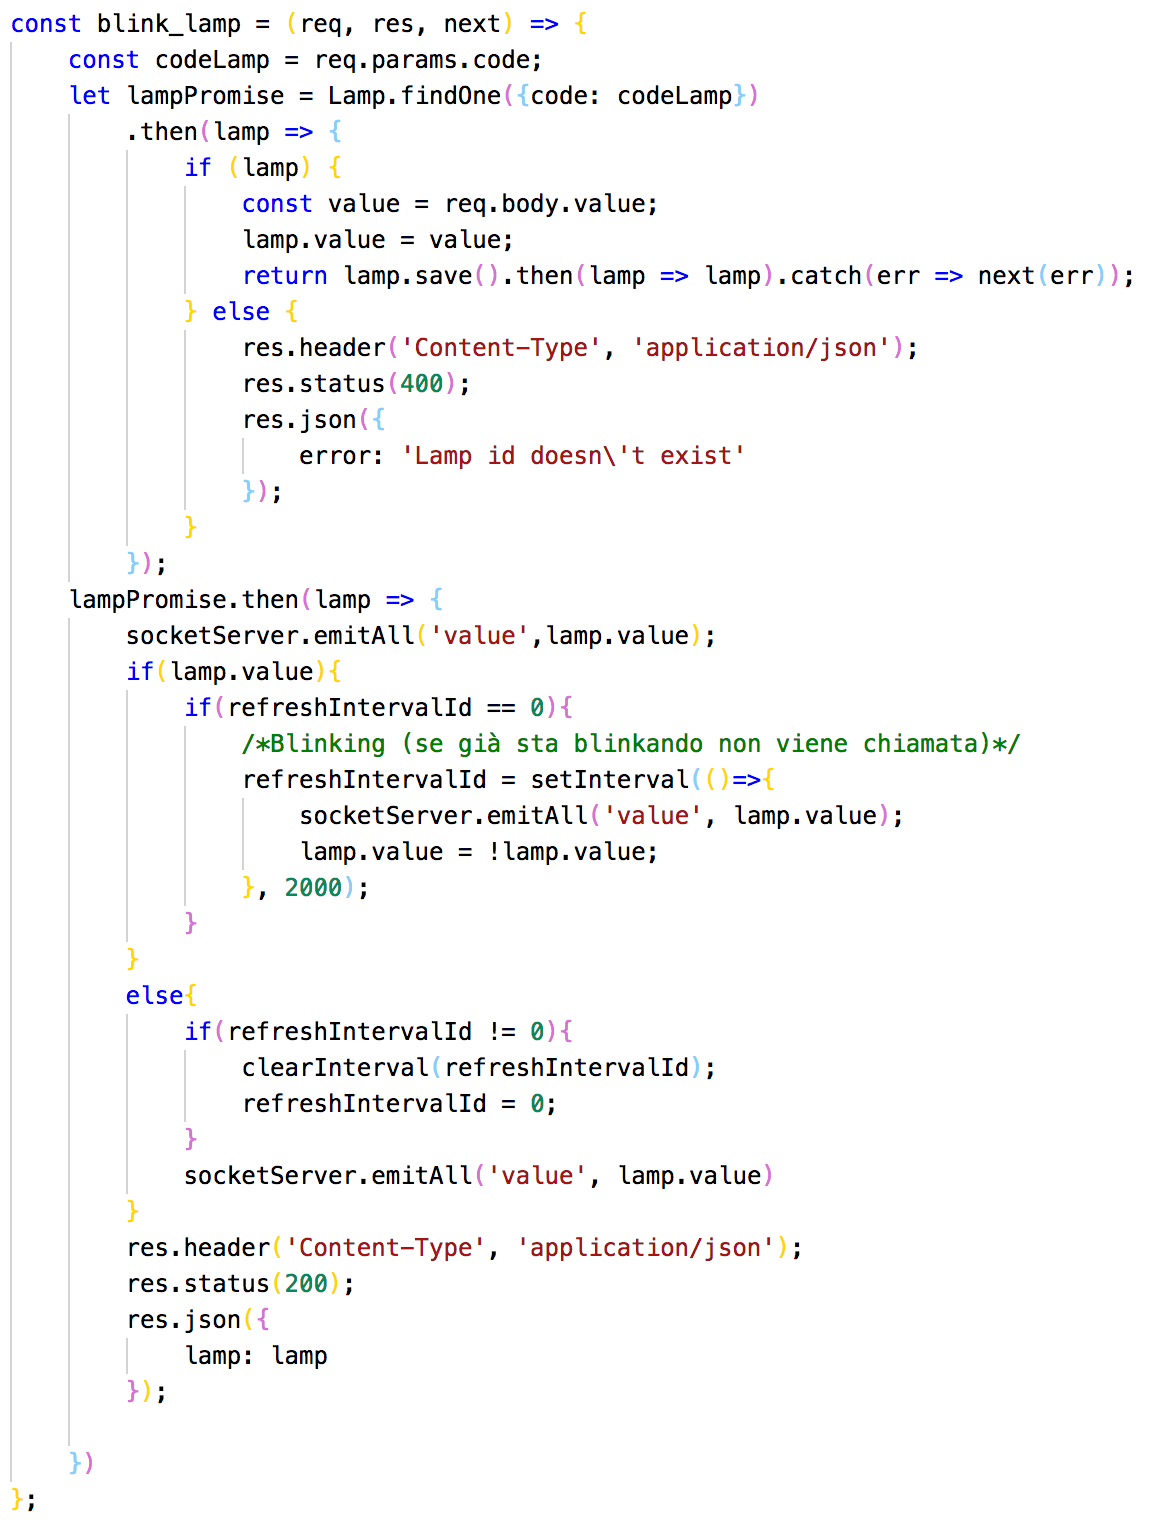
\includegraphics[width=0.8\textwidth]{Immagini/Requisito4/BlinkLamp.png}
    \caption{Codice della gestione della richiesta (web server)}
    \label{fig:CodeWebServerReq4}
\end{figure}
\vspace*{1ex}
\\
% Implementazione: Script Python ======================================================================
\subsubsection{Implementazione: Script Python} .
\label{ImplementazioneReq4ScriptPython}
\vspace*{1ex}
\\
Al lancio di questo script dovr\`a essere specificato se il led, sul quale si vuole compiere un'azione (accensione o spegnimento), \`e quello posto sulla raspberry o quello posto all'interno della casa (Led Hue Lamp). Proprio per questo motivo nei paragrafi successivi verranno introdotti due script che descrivano queste azioni.\\
Una volta lanciato, lo script aprir\`a una socket con il web server e si metter\`a in attesa di un comando. Ogni volta che sar\`a presente un valore sulla socket verr\`a richiamata una \textbf{callback}, a seconda del led specificato, che effettuer\`a  l'operazione richiesta. Questa parte verr\`a trattata nel dettaglio nei paragrafi successivi.\\
\begin{figure}
    \centering
    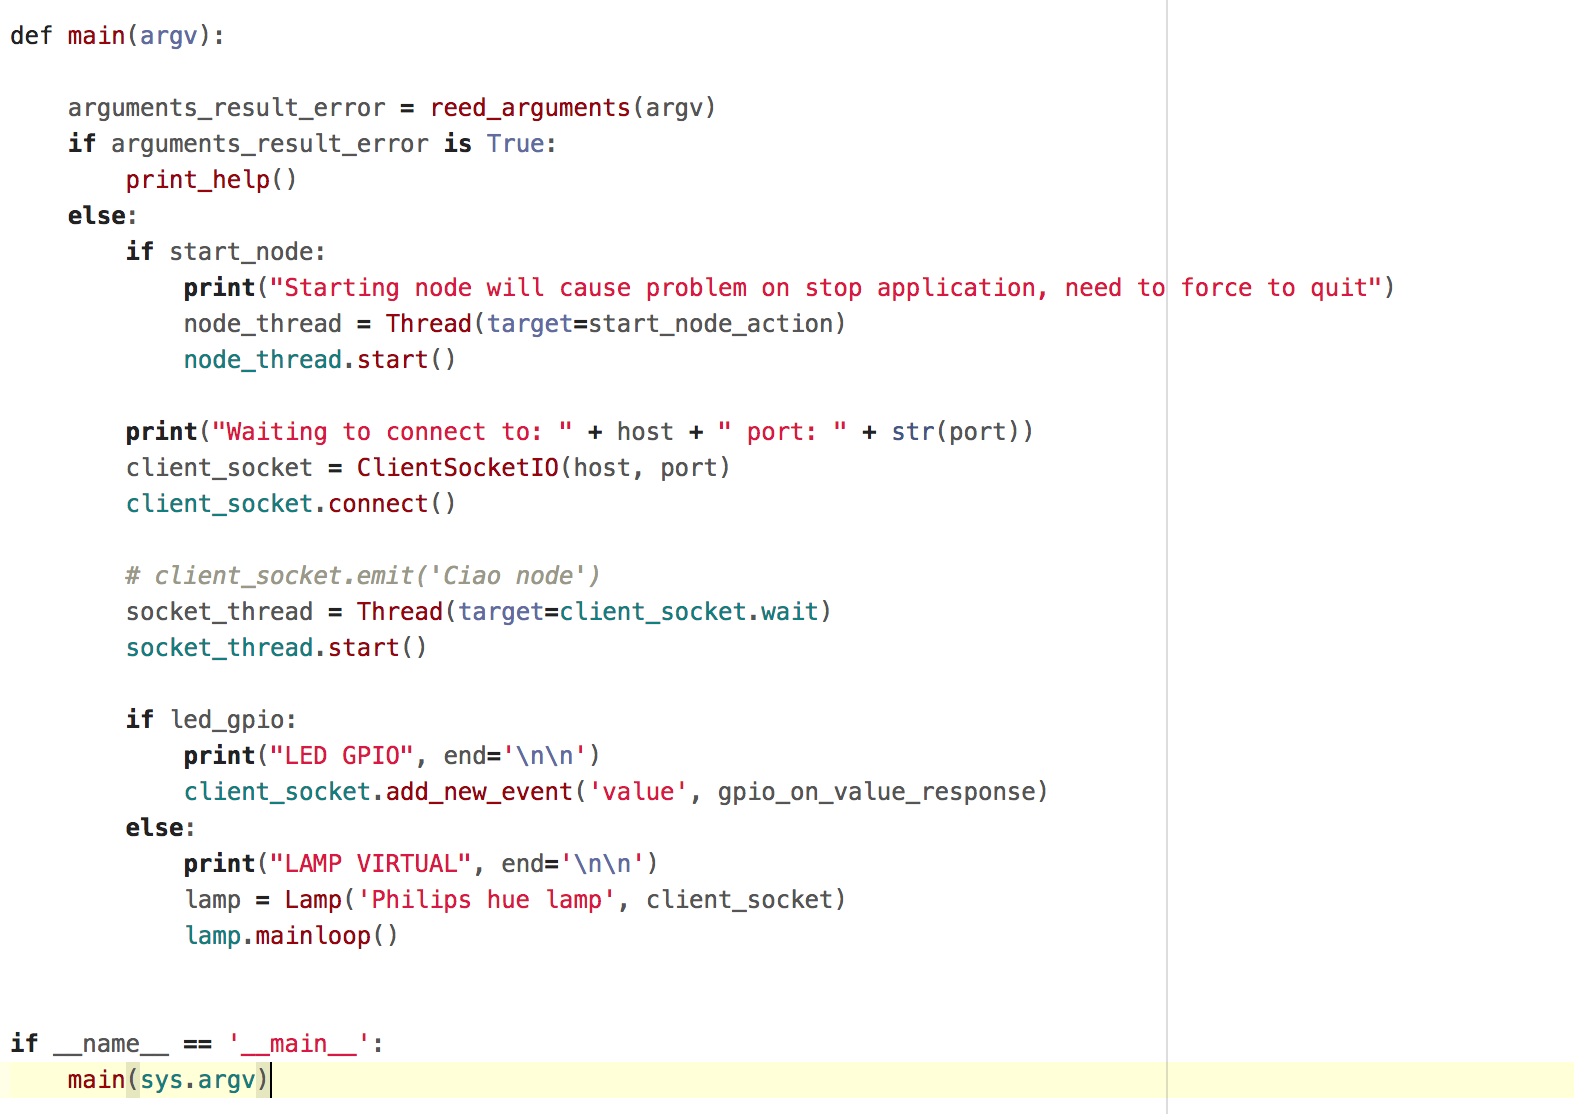
\includegraphics[width=1\textwidth]{Immagini/Requisito4/pythonScriptReq4.png}
    \caption{Main Script python}
    \label{fig:MSpython}
\end{figure}
\vspace*{1ex}
\\
% Implementazione: Led  ======================================================================
\subsubsection{Implementazione: Led} .
\label{ImplementazioneReq4Led}
\vspace*{1ex}
\\
In questa implementazione, realizzata anch'essa in \textbf{python}, sono presenti due funzioni: una per accendere e una per spegnere il led. Entrambe verranno invocate dalla funzione di callback, impostata nello script python iniziale, che, una volta ricevuto il comando, stabilir\`a quale sar\`a la funzione da invocare.\\
\begin{figure}
    \centering
    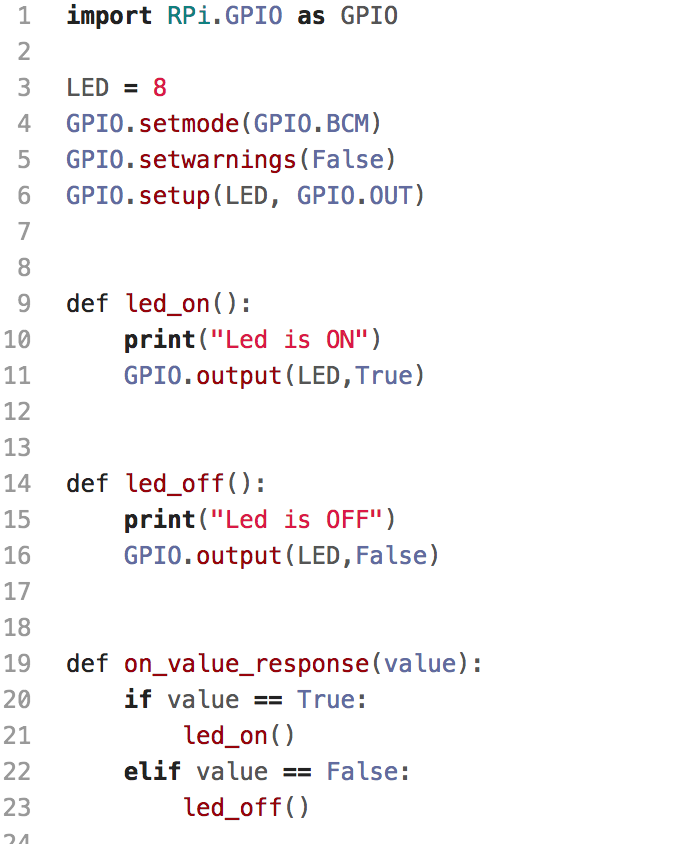
\includegraphics[width=0.5\textwidth]{Immagini/Requisito4/LedGPIOReq4.png}
    \caption{Led Robot Reale}
    \label{fig:LRR}
\end{figure}
\vspace*{1ex}
\\
Per accedere ai PIN della raspberry in python esiste la libreria GPIO che, una volta stabilita la modalit\`a di accesso (nel nostro caso \textbf{BCM} Broadcom SOC channel), permette di stabilire se accedervi in INPUT o in OUTPUT. Nel nostro caso il PIN dove il led \`e posto \`e il numero 8; questo sar\`a quindi impostato in OUTPUT.\\
Una volta effettuate le operazioni sopra elencate, le funzioni useranno la libreria GPIO per impostare il valore del PIN.

% Implementazione: Simulazione Led Hue Lamp ======================================================================
\subsubsection{Implementazione: Simulazione Led Hue Lamp} .
\label{ImplementazioneReq4LHL}
\vspace*{1ex}
\\
L'implementazione del \textbf{Led Hue Lamp} richiesto dal committente ha necessitato la creazione di un componente mock che simulasse il comportamento di tale lampadina, in quanto quest'ultima non \`e attualmente disponibile nella nostra software house.\\
La Led Hue Lamp mock \`e quindi stata realizzata in \textbf{python}, in quanto era gi\`a stato previsto un ambiente python in grado di comunicare con il web server per l'accensione del led fisico tramite i pin GPIO; quindi \`e stata realizzata una classe che utilizza il package grafico di python (\textbf{tkinter}) per creare una finestra di piccole dimensioni (70px) che simuli una lampadina spenta. Questa classe prevede poi un metodo da invocare quando si vuole accendere la lampada che va ad aumentare la dimensione della finestra (a 500px, lampadina accesa).\\
Infine in questa classe nel costruttore viene impostata la callback, invocata al presentarsi di un valore sulla socket definita nello script python(\hyperref[ImplementazioneReq4ScriptPython]{\ref{ImplementazioneReq4ScriptPython}}), che permetter\`a di modificare la dimensione della finestra.\\
\begin{figure}
    \centering
    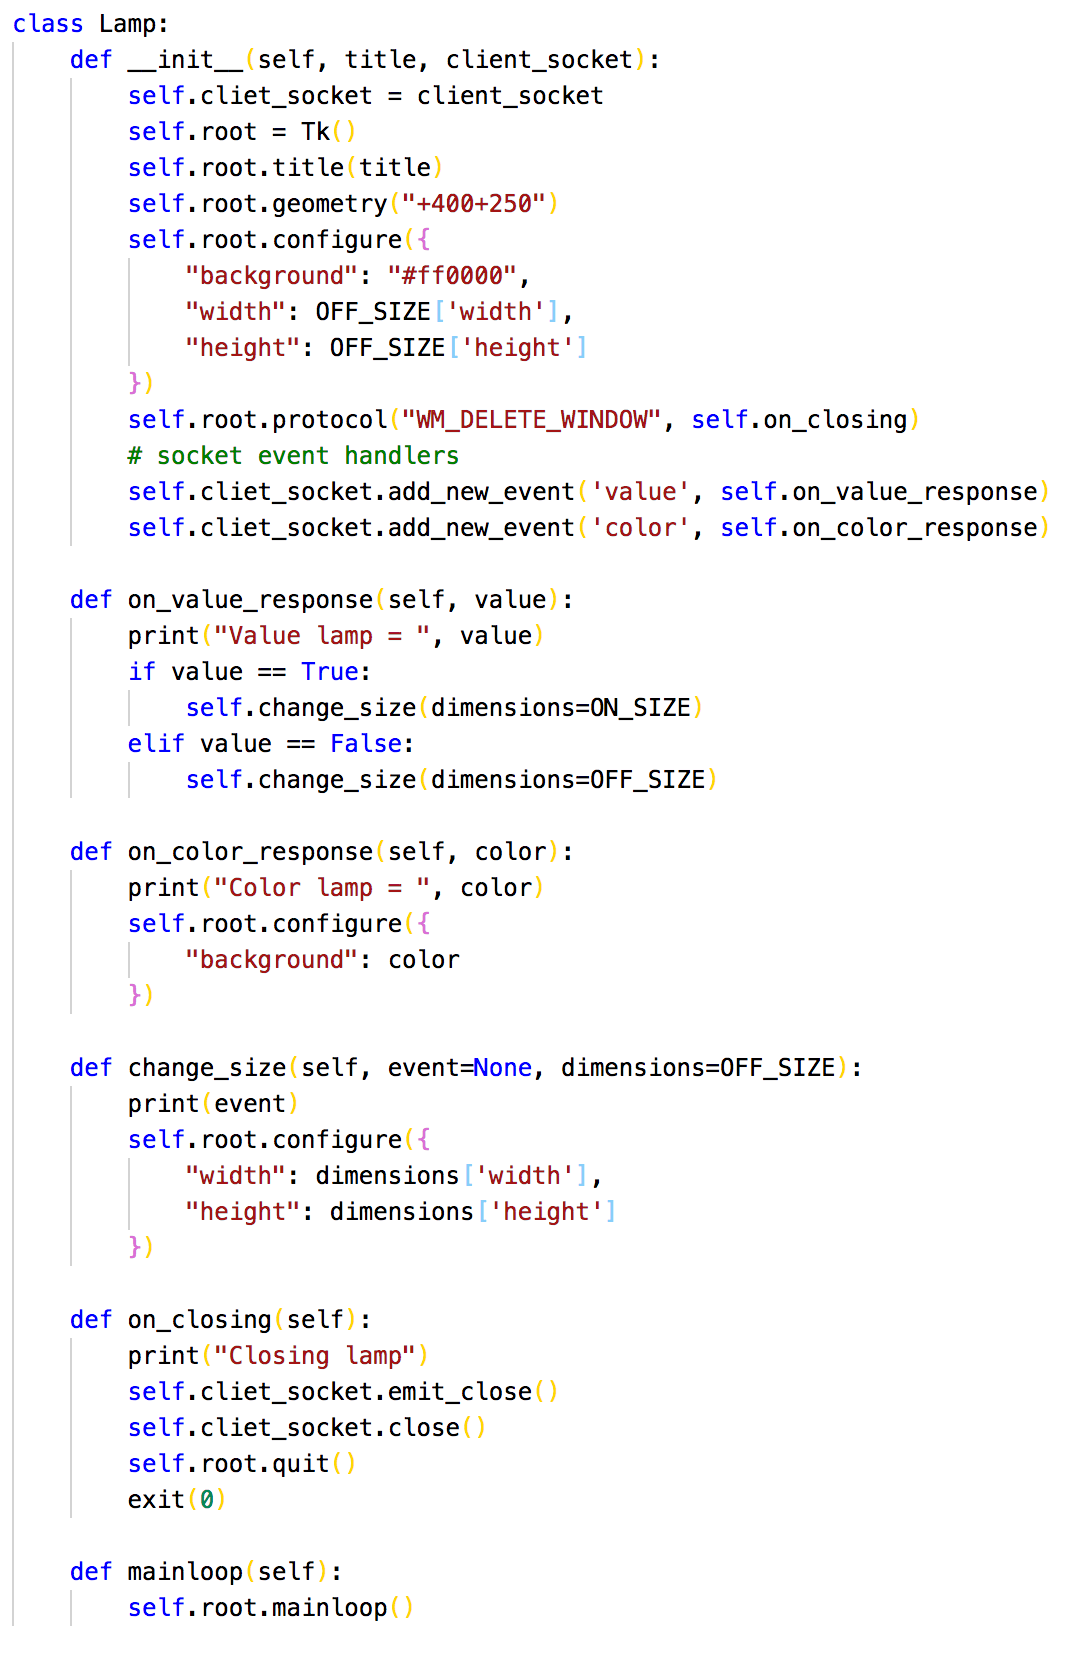
\includegraphics[width=0.8\textwidth]{Immagini/Requisito4/PythonHUELamp.png}
    \caption{Classe della lampadina HUE}
    \label{fig:ClasseLHL}
\end{figure}
\vspace*{1ex}
\\
\pagebreak

%Requisito 4: Pregettazione: Refactoring ========================================================
\subsection{Progettazione: Refactoring}
\label{ProgettazioneRefReq4}
Dopo aver realizzato un ulteriore prototipo funzionante per il committente, ci siamo resi conto che una soluzione migliore sarebbe stata quella di estrarre la base di conoscenza dalla mind. In questo modo la mind avrebbe avuto un carico applicativo ridotto, ma sarebbe comunque riuscita ad accedere a tutte le informazioni essenziali di tutti i componenti; un ulteriore vantaggio sarebbe stato quello di poter separare la base di conoscenza dalla logica applicativa.\\
La base di conoscenza verr\`a quindi inserita all'interno di un file Prolog chiamato \textbf{Resource model} (modello delle risorse). La struttura della mind diventer\`a quella illustrata in figura \hyperref[fig:MindRMReq4]{\ref{fig:MindRMReq4}}.\\
\begin{figure}
    \centering
    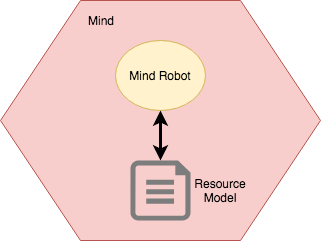
\includegraphics[width=0.5\textwidth]{Immagini/Requisito4/MindWithResourceModel.png}
    \caption{Mind con resource model}
    \label{fig:MindRMReq4}
\end{figure}
\vspace*{1ex}
\\
%Requisito 4: Implementazione: Refactoring ========================================================
\subsection{Implementazione: Refactoring}
\label{ImplementazioneRefReq4}
La mind, separata dalla base di conoscenza (le Rules), al suo avvio dovr\`a caricare nel sistema il file Prolog definito \textbf{Resource model} in fase di progettazione (Fig. \hyperref[fig:MindConsultRMReq4]{\ref{fig:MindConsultRMReq4}}).
\\
\begin{figure}
    \centering
    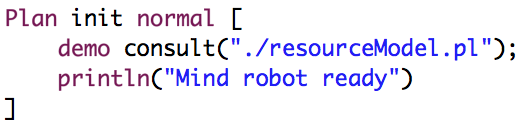
\includegraphics[width=0.5\textwidth]{Immagini/Requisito4/ResourceModelConsult.png}
    \caption{Mind inizializza il resource model}
    \label{fig:MindConsultRMReq4}
\end{figure}
\vspace*{1ex}
\\
Il resource model si compone principalmente di 3 parti:
\begin{itemize}
    \item La prima contiene lo stato dei componenti (o risorse) del sistema \textbf{Model} e un predicato da usare per leggere questi valori (Fig. \hyperref[fig:ModComp]{\ref{fig:ModComp}});
    \item La seconda prevede un predicato (\textbf{changeModelItem}) da utilizzare ogni volta che si vuole modificare uno dei modelli presenti nella prima parte (Fig. \hyperref[fig:CMI]{\ref{fig:CMI}});
    \item La terza contiene le azioni da eseguire quando uno delle propriet\`a del model viene modificata. Queste azioni verranno usate per verificare la correttezza dei vincoli (inseriti nei requisiti precedenti) e per notificare il sistema degli eventuali cambiamenti (tramite l'emissione di eventi).
\end{itemize}
\begin{figure}
    \centering
    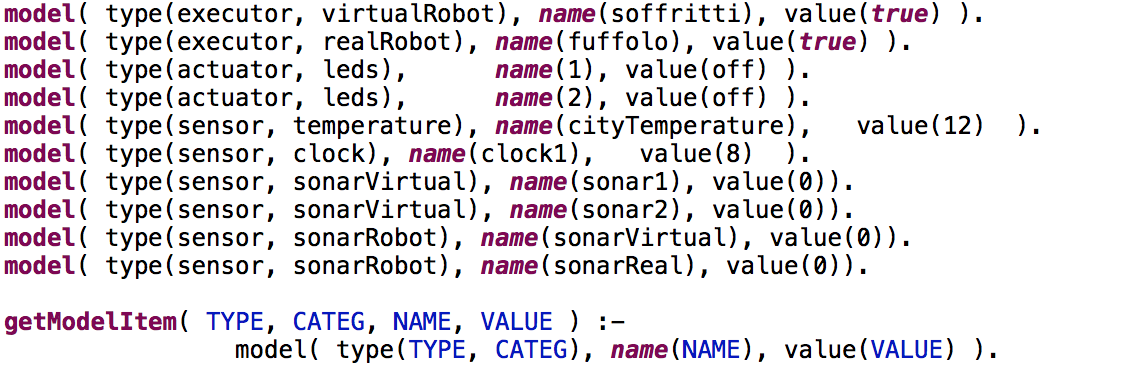
\includegraphics[width=0.8\textwidth]{Immagini/Requisito4/modelliResModReq4.png}
    \caption{Modelli delle componenti}
    \label{fig:ModComp}
\end{figure}
\vspace*{1ex}

\begin{figure}
    \centering
    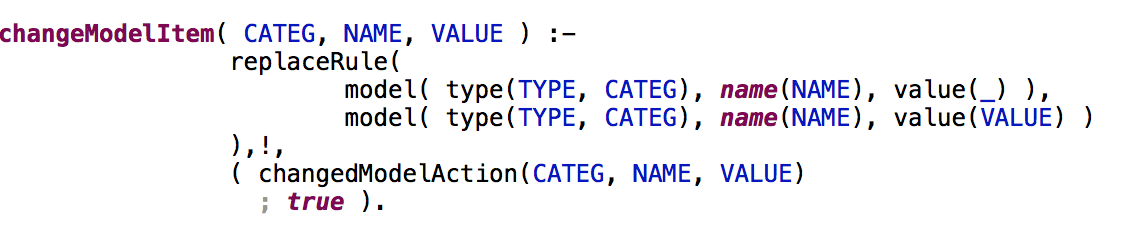
\includegraphics[width=1\textwidth]{Immagini/Requisito4/changeMIReq4.png}
    \caption{Change Model Item}
    \label{fig:CMI}
\end{figure}
\vspace*{1ex}

\begin{figure}
    \centering
    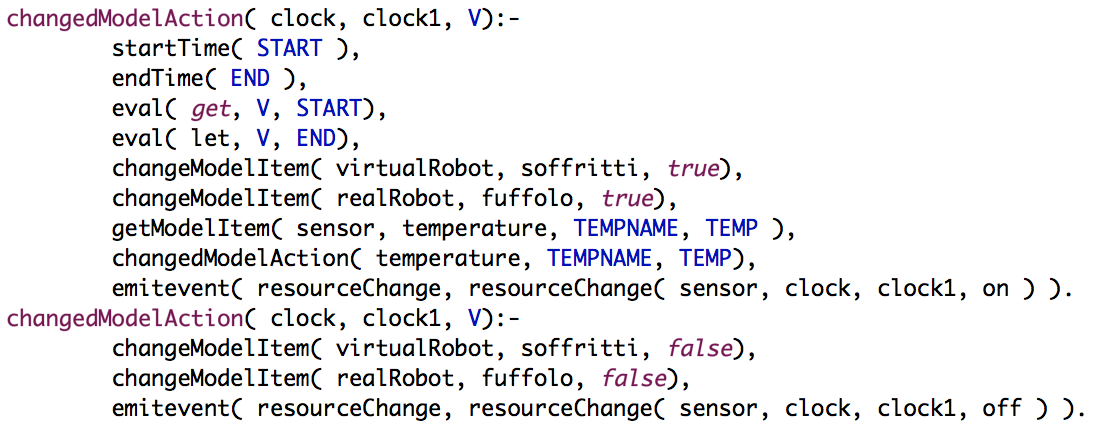
\includegraphics[width=1\textwidth]{Immagini/Requisito4/ChangedModelAction.png}
    \caption{Esempio Change Model Action}
    \label{fig:CMAEx}
\end{figure}
Introducendo questa separazione, i controlli, precedentemente definiti nella base di conoscenza, non saranno invocati direttamente dalla mind, ma soltanto al verificarsi di un cambiamento all'interno del Resource model. Al cambiamento di una risorsa ( \texttt{changeModelItem -> changeModelAction}) verr\`a scatenato un evento che segnaler\`a alla mind il cambiamento effettuato.

\subsubsection{Implementazione: Refactoring console}.
\label{ImplementazioneRefConsoleReq4}
\vspace*{1ex}
\\
Il refactoring apportato nel sistema PER introdurre il Resource model ha causato la modifica della console, in quanto per rendere il prodotto pi\`u appetibile sul mercato \`e necessario prevedere la duplicazione delle informazioni relative alle risorse presenti nella Mind anche nel Web Server della console per mostrarle nella GUI dell'utente. Queste informazioni verranno duplicate per garantire il funzionamento dei due componenti (Console e Mind) in maniera indipendente l'uno dall'altro.\\
Per implementare questa duplicazione la Mind, ogni volta che ci sar\`a una modifica del suo modello interno, notificher\`a il Web Server node emettendo su MQTT un evento (\texttt{resourceChangeEvent}) il cui payload conterr\`a le informazioni da modificare. Il Web Server rilever\`a questi eventi e provveder\`a ad aggiornare il proprio Resource model, salvando queste nuove informazione in opportune tabelle del suo DataBase. Infine il Web Server notificher\`a la GUI React della modifica delle risorse, in modo tale che l'interfaccia poss\`a ricaricare le informazioni aggiornate e mostrarle all'utente (Fig. \hyperref[fig:RMGUI]{\ref{fig:RMGUI}}).
\begin{figure}
    \centering
    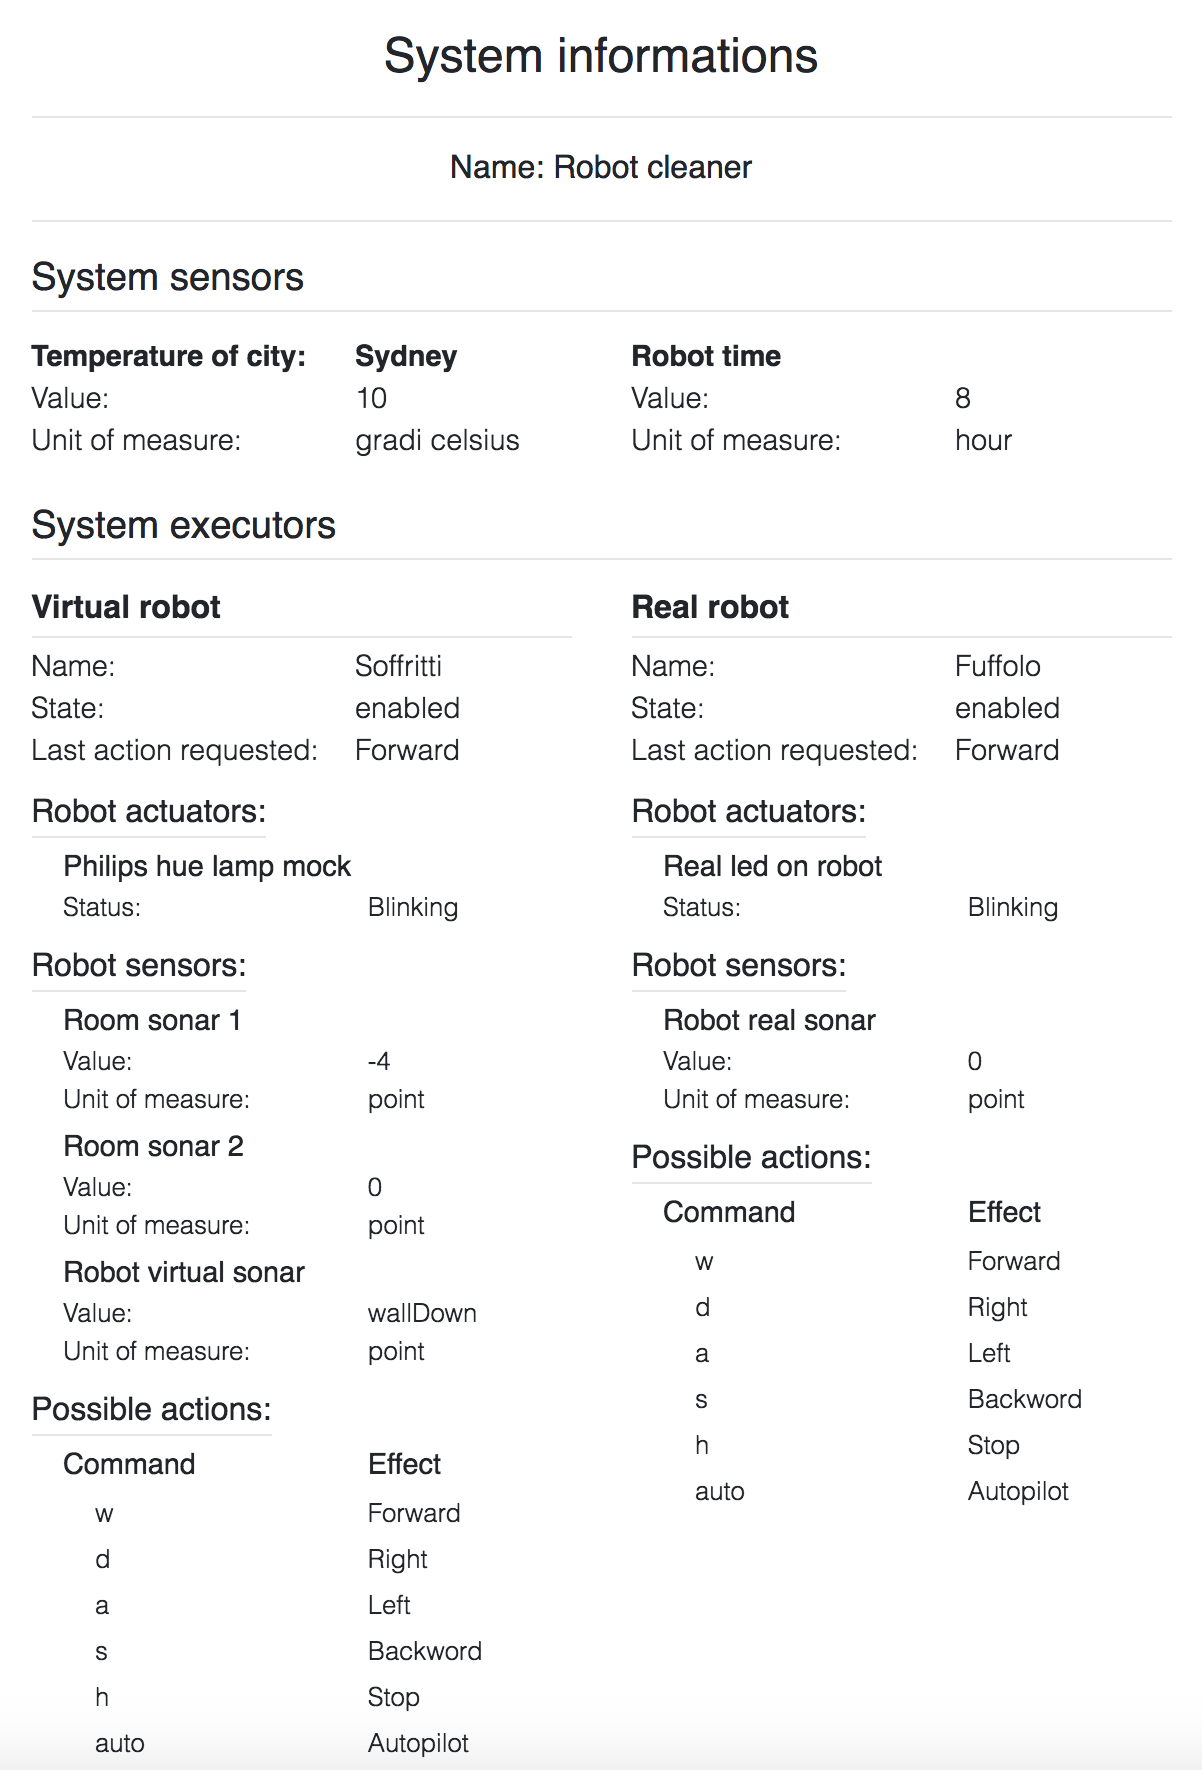
\includegraphics[width=0.7\textwidth]{Immagini/Requisito4/ResourceModelGui.png}
    \caption{Stampa sulla GUI del Resource model}
    \label{fig:RMGUI}
\end{figure}

\pagebreak
%Requisito 5 =========================================================================
\section{Requisito 5}
\label{Requisito5}
Durante l'analisi del problema del precedente requisito abbiamo rimandato ad fase successiva l'analisi e l'implementazione della funzionalit\`a che permette ai robot di evitare gli ostacoli. Questo perch\`e abbiamo pensato di integrare quest'ultima con quella relativa all'ultimo requisito, ovvero la costruzione della mappa di una stanza in cui possono essere presenti degli ostacoli.\\

%Analisi del problema 5: mappa =========================================================================
\subsection{Analisi del problema: mappa}
\label{AnalisiReq5}
Per poter realizzare la mappa durante il processo di pulizia della stanza il robot deve riuscire in qualche modo a tener traccia dei movimenti che effettua.\\
Abbiamo deciso di procedere dividendo la mappa della stanza in celle che caratterizzano una matrice, dove ogni cella corrisponde alla dimensione del robot. Per fare ci\`o occorre tenere in considerazione i seguenti fattori:
\begin{itemize}
    \item La posizione iniziale del robot;
    \item La dimensione di una cella;
    \item Disegnare la mappa come un insieme di celle (cos\`i da capire se il robot ha coperto tutta la stanza);
    \item La posizione iniziale deve essere un angolo della stanza; \label{cons1}
    \item Sui due lati iniziali della stanza non ci devono essere ostacoli.\label{cons2}
\end{itemize}
\begin{figure}
    \centering
    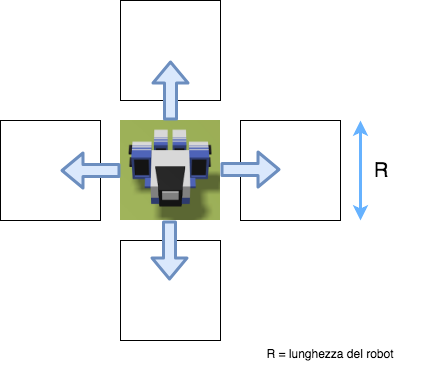
\includegraphics[width=0.4\textwidth]{Immagini/Requisito5/RobotDirections.png}
    \caption{Dimensione della cella}
    \label{fig:R5DimCella}
\end{figure}
La \textbf{posizione iniziale} del robot \`e rappresentata dalla posizione che occupa nella stanza al momento dell'inizio della pulizia ed \`e equivalente alla posizione del sonar 1.\\
La \textbf{dimensione della cella}, rappresentata dalla dimensione del robot, ci aiuter\`a a capire quali sono gli step che il robot dovr\`a eseguire. La \textbf{dimensione del robot}, come illustrato nella figura \hyperref[ig:R5DimCella]{\ref{fig:R5DimCella}} , \`e rappresentata da un valore R che - una volta definito - ci consentir\`a di stabilire per quanti millisecondi il robot deve muoversi ad una certa velocit\`a costante v per effettuare uno step, ovvero l'attraversamento di una cella. Per il calcolo di questo valore R ci siamo spostati direttamente sull’applicazione del virtual robot, usando il file javascript clientTest messo a disposizione dalla nostra software house. Dalle prove risulta che il valore corretto \`e di \textbf{200ms}, questo significa che gli step che il robot dovr\`a effettuare sono di 200ms. Ovviamente le stesse prove sono state effettuate anche sul real robot.\\
Per andare a disegnare la mappa della stanza useremo il numero di celle occupate dal robot fino al raggiungimento del primo ostacolo e il segnale ricevuto dal secondo sonar. Una volta raggiunta questa posizione il robot proceder\`a verso il secondo sonar contando il numero di passi effettuati, cos\`i da ottenere la dimensione effettiva della stanza.\\
La nostra software house ci fornisce anche un \textbf{planner} che, data la dimensione della stanza, definir\`a  il piano che il robot dovr\`a eseguire per pulire la stanzanella sua interezza.\\
Il \textbf{planner} \`e un agente software che tiene traccia del percorso gi\`a effettuato dal robot e che \`e in grado di restituire la mossa successiva da effettuare in base alla mappa corrente.
%Arrivati a questo punto il robot conoscer\`a la dimensione della stanza e quindi ne avr\`a la mappa, ovviamente supponendo che la stanza sia un rettangolo o un quadrato.\\
\begin{figure}
    \centering
    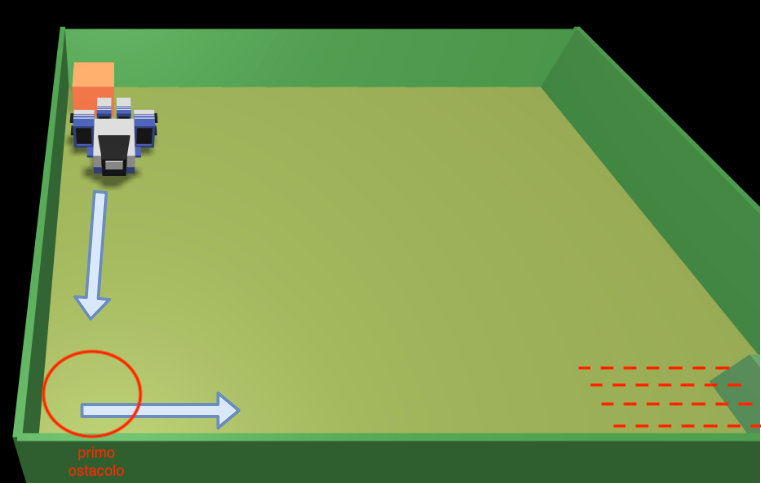
\includegraphics[width=0.8\textwidth]{Immagini/Requisito5/RobotStart.png}
    \caption{Posizione iniziale del robot}
    \label{fig:R5StartingPoint}
\end{figure}\\

%Analisi del problema 5: Ostacoli =========================================================================
\subsubsection{Analisi del problema: Ostacoli}.
\label{AnalisiReq5Ostacoli}
\vspace*{1ex}
\\
Durante la creazione della mappa - e quindi durante la pulizia della stanza - il robot deve essere in grado di evitare gli ostacoli, come specificato nel requisito 4 (paragrafo \hyperref[ReqAnalysis4]{\ref{ReqAnalysis4}}), facendo distinzione tra gli ostacoli mobili e quelli fissi in quanto solo quest'ultimi devono essere segnati anche nella mappa.\\
Gi\`a in questa fase si individua la nostra strategia da utilizzare per distinguere il tipo di ostacolo. Questa consiste nel tentare, un numero prefissato di volte, di andare avanti come se non ci fossero impedimenti. Se durante questi tentativi riusciremo a superare l'ostacolo, vorr\`a dire che quest'ultimo \`e mobile e quindi ignorabile; se invece al termine di questi tentativi l'ostacolo \`e ancora rilevato, possiamo assumere, con grande probabilit\`a, che quello sia un ostacolo fisso e che quindi andr\`a segnato anche sulla mappa.

%Progettazione Requisito 5 =========================================================================
\subsection{Progettazione}
\label{ProgettRazioneReq5}
Da quanto dedotto dall'analisi del problema ci servir\`a qualcosa che vada ad effettuare le operazioni iniziali, ovvero portare il robot dalla posizione iniziale al secondo sonar seguendo i passi indicati in precedenza. Da qui si capisce la necessit\`a delle ultime due considerazioni iniziali fatte in analisi del problema: la posizione iniziale deve essere un angolo della stanza e sui due lati iniziali della stanza non ci devono essere ostacoli.\\
Una volta che il robot avr\`a raggiunto il secondo sonar (end-point) ed avr\`a calcolato la dimensione della mappa, il metodo che si occuper\`a della sua costruzione dovr\`a far partire il planner fornitoci dalla nostra software house.
\begin{figure}
    \centering
    \includegraphics[width=0.8\textwidth]{Immagini/Requisito5/SecondSonarVirtual.png}
    \caption{Virtual Robot sul secondo sonar}
    \label{fig:R5VirtualOnSecondSonar}
\end{figure}
L'architettura finale una volta che l'utente avr\`a ottenuto l'autorizzazione \`e quella mostrata in figura \textbf{\hyperref[fig:finalstructure]{\ref{fig:finalstructure}}}.
\begin{figure}
    \centering
    \includegraphics[width=0.8\textwidth]{Immagini/Requisito5/SystemStructure.png}
    \caption{Struttura finale}
    \label{fig:finalstructure}
\end{figure}
\pagebreak
%Implementazione Requisito 5 =========================================================================
\subsection{Implementazione}
\label{ImplementazioneReq5}

%Implementazione: Mind=========================================================================
\subsubsection{Implementazione: Mind}.
\label{ImplementazioneMindReq5}
\vspace*{1ex}
\\
Durante l'implementazione di questo requisito si \`e deciso di effettuare un piccolo refactoring al \qa della Mind in quanto volevamo dare una separazione pi\`u netta tra la logica applicativa e l'esecuzione dei comandi del robot. Perci\`o sono stati aggiunti due nuovi attori che rimarranno interni al contesto della Mind:
\begin{itemize}
    \item \texttt{delegateexecutor} usato solamente per inviare su MQTT i messaggi per muovere i robot; esso comunicher\`a a sua volta con la Mind tramite messaggi  (ID messaggio: \texttt{exec});
    \item \texttt{autopilot} questo \qa \`e stato creato solamente per motivi implementativi in quanto il metodo statico Java usato per avviare il pilota automatico risulta essere bloccante (se lanciato all'interno della Mind non si sarebbe potuto eseguire nessun altro comando); anch'esso comunica con la Mind tramite messaggi (ID messaggio: \texttt{exec})
\end{itemize}
Nella Mind \`e stata necessaria anche un'ulteriore modifica per utilizzare il pilota automatico, ovvero si \`e dovuto aggiungere nel gestore dei messaggi un controllo per rilevare il comando - \texttt{usercmd( robotgui(auto(X)) )}- inviato dalla Console per far avviare l'auto pilot (Fig. \hyperref[fig:R5AutoPilotMind]{\ref{fig:R5AutoPilotMind}} ). 
\begin{figure}
    \centering
    \includegraphics[width=1\textwidth]{Immagini/Requisito5/AutoPilotMind.png}
    \caption{Rilevamento del comando di auto pilot dalla Console}
    \label{fig:R5AutoPilotMind}
\end{figure}
\pagebreak
%Implementazione: AutoPilot=========================================================================
\subsubsection{Implementazione: Auto Pilot (Start command)}.
\label{ImplementazioneAutoPilotReq5}
\vspace*{1ex}
\\
Nell'analisi del problema e nella progettazione abbiamo stabilito che, per stabilire la dimensione della mappa, il robot inizialmente deve effettuare dei movimenti prefissati (vedi Figura \hyperref[fig:R5StartingPoint]{\ref{fig:R5StartingPoint})}. Per fare questi movimenti, all'interno della classe \java che descrive l'autopilot, sono stati definiti due metodi:
\begin{enumerate}
    \item Il primo permette al robot di arrivare fino al primo ostacolo che corrisponde al primo muro della stanza;
    \item Il secondo, oltre a permettere al robot di arrivare al secondo sonar, di volta in volta effettua un rotazione a destra e uno step in avanti, in modo tale che possa tracciare meglio la mappa della stanza. In questo modo il \textbf{planner} avr\`a pi\`u informazioni sulla stanza e quindi sar\`a pi\`u preciso.
\end{enumerate}
\begin{figure}
    \centering
    \includegraphics[width=1\textwidth]{Immagini/Requisito5/forwardToObstacle.png}
    \caption{Primo Metodo}
    \label{fig:forwardToObstacle}
\end{figure}
\begin{figure}
    \centering
    \includegraphics[width=1\textwidth]{Immagini/Requisito5/traceMap.png}
    \caption{Secondo Metodo}
    \label{fig:secondoMetodo}
\end{figure}
Dopo aver realizzato questi due metodi ci siamo resi conto che i sonar erano nel nostro caso inutili, in quanto le verifiche sul fatto che la mossa generata dal planner fosse applicabile o fosse una mossa che portava contro un ostacolo fisso venivano fatte prima di muovere realmente il robot (Fig. \hyperref[fig:clearRoom]{\ref{fig:clearRoom}}). Questo ci consentiva, in caso di collisione, di aggiornare la mappa e quindi di richiedere al planner la prossima mossa valida.\\
\begin{figure}
    \centering
    \includegraphics[width=1\textwidth]{Immagini/Requisito5/clearRoom.png}
    \caption{Metodo che utilizza il planner}
    \label{fig:clearRoom}
\end{figure}
Una volta realizzati questi metodi l'autopilot dovr\`a semplicemente richiamarli in sequenza (Fig. \hyperref[fig:autopilot]{\ref{fig:autopilot}}) .\\
\begin{figure}
    \centering
    \includegraphics[width=1\textwidth]{Immagini/Requisito5/AutoPilot.png}
    \caption{Start AutoPilot}
    \label{fig:autopilot}
\end{figure}

%Implementazione: ostacoli =========================================================================
\subsubsection{Implementazione: Ostacoli}.
\label{ImplementazioneOstacoliReq5}
\vspace*{1ex}
\\
L'implementazione del meccanismo per evitare e categorizzare gli ostacoli richiede l'interazione tra 3 componenti del sistema:
\begin{itemize}
    \item La Mind sar\`a responsabile di intercettare gli eventi emessi su MQTT dai robot relativi al rilevamento di un ostacolo (\texttt{sonarDetect} nel caso del robot virtuale e \texttt{realSonarDetect} nel caso del robot reale).\\
    Una volta che la Mind avr\`a analizzato l'evento ricevuto dovr\`a modificare il Resource Model mediante il comando \texttt{demo changeModelItem(CATEG, NAME, VALUE)}, come \`e evidenziato dalla figura \hyperref[fig:R5HandleSonarChange]{\ref{fig:R5HandleSonarChange}};
    \item Il Resource model sar\`a responsabile di aggiornare la base di conoscenza del sistema in maniera da consentire agli altri componenti di verificare la presenza o meno di ostacoli. Per farlo, quando verr\`a invocato dalla Mind il predicato \texttt{changeModelItem(CATEG, NAME, VALUE)}, si andr\`a a modificare il valore del fatto \texttt{model( type(sensor, obstacle), name(sonar), value(no)).} inserendo il valore \texttt{yes} nel caso di \textbf{Robot Virtuale}, mentre nel caso di \textbf{Robot Reale} il valore \texttt{yes} verr\`a inserito solo se la distanza da un ostacolo \`e minore di una certa soglia (40cm), come si pu\`o notare nella figura \hyperref[fig:R5RMHandleSonarChange]{\ref{fig:R5RMHandleSonarChange}};
    \item Un metodo statico custom, che viene invocato dalla funzione di pilota automatico, deve verificare se l'ostacolo rilevato \`e statico o mobile; questo metodo controller\`a per tre volte, a distanza di un certo intervallo, se l'ostacolo \`e ancora presente. Ad ogni iterazione il metodo prova ad avanzare di uno step, richiede al Resource model se ha trovato un ostacolo verificando il fatto \texttt{model( type(sensor, obstacle), name(sonar), value(VALUE)).} Se \texttt{VALUE} ha val,ore \texttt{yes} allora si reimposta il valore a \texttt{no} e si ripete il ciclo altrimenti ferma l'iterazione e comunica che l'ostacolo \`e dinamico. Se l'iterazione viene ripetuta per tre volte l'ostacolo verr\`a considerato statico (Fig. \hyperref[fig:R5ObstacleIsStatic]{\ref{fig:R5ObstacleIsStatic}}).
\end{itemize}
\begin{figure}
    \centering
    \includegraphics[width=1\textwidth]{Immagini/Requisito5/HandleSonarChangeQA.png}
    \caption{Gestione degli eventi \texttt{sonarDetec} e \texttt{realSonarDetect}}
    \label{fig:R5HandleSonarChange}
\end{figure}
\begin{figure}
    \centering
    \includegraphics[width=1\textwidth]{Immagini/Requisito5/RMSonarRobotChange.png}
    \caption{Resource model: modifica del fatto \texttt{model( type(sensor, obstacle), name(sonar), value(no)).}}
    \label{fig:R5RMHandleSonarChange}
\end{figure}
\begin{figure}
    \centering
    \includegraphics[width=1\textwidth]{Immagini/Requisito5/ObstacleIsStatic.png}
    \caption{Metodo per controllare se un ostacolo \`e statico}
    \label{fig:R5ObstacleIsStatic}
\end{figure}

\pagebreak

%Implementazione: map GUI =========================================================================
\subsubsection{Implementazione: Mappa sulla GUI}.
\label{ImplementazioneMappaGUIReq5}
\index{Implementazione: Mappa sulla GUI}
\vspace*{1ex}
\\
La rappresentazione della mappa \`e stata fatta non solo all'interno del sistema Robot ma anche nella GUI dell'untente per rendere il tutto pi\`u appetibile sul mercato; perci\`o il metodo del pilota automatico ad ogni nuova mossa effettuata invia lo stato attuale dell'intera mappa al Web Server node che provveder\`a a salvare la mappa nel suo database e inviare quest'ultima alla GUI Reac. In questo modo sar\`a visualizzata direttamente sul dispositivo dell'utente in modo da mostrare l'avanzamento del robot passo dopo passo (Fig. \hyperref[fig:R5GUIMAP]{\ref{fig:R5GUIMAP}}).
\begin{figure}
    \centering
    \includegraphics[width=0.4\textwidth]{Immagini/Requisito5/MapDirty.png}
    \includegraphics[width=0.4\textwidth]{Immagini/Requisito5/MapClean.png}
    \caption{Stanza ancora sporca figura di sinistra, Stanza pulita figura di destra}
    \label{fig:R5GUIMAP}
\end{figure}
\pagebreak

%Requisito 5 =========================================================================
\section{Autori}
\label{Autori}
\begin{figure}
    \centering
    \includegraphics[width=0.3\textwidth]{Immagini/autore.jpeg}
    \includegraphics[width=0.5\textwidth]{Immagini/Alessandro.jpg}
    \caption{Angelo Feraudo, Alessandro Staffolani}
    \label{fig:my_label}
\end{figure}
Link al repository github: \url{https://github.com/ale8193/robot-cleaner}
\end{document}












